\documentclass[a4paper, 11pt, oneside]{article}
\usepackage{lmodern}
\usepackage[T1]{fontenc}
% Load encoding definitions (after font package)
\usepackage{textalpha}

\usepackage[dvipsnames]{xcolor}
\usepackage{eso-pic,graphicx}
\usepackage[top=50mm, bottom=50mm, outer=29mm, inner=29mm]{geometry}
\setlength{\columnsep}{90pt}

% Babel package:
\usepackage[main=german,polutonikogreek]{babel}
\usepackage{listings}
\lstset{basicstyle=\ttfamily}

% With XeTeX$\$LuaTeX, load fontspec after babel to use Unicode
% fonts for Latin script and LGR for Greek:
\ifdefined\luatexversion \usepackage{fontspec}\fi
\ifdefined\XeTeXrevision \usepackage{fontspec}\fi

% "``Lipsiakos"' italic font `cbleipzig`:
\newcommand*{\lishape}{\fontencoding{LGR}\fontfamily{cmr}%
		       \fontshape{li}\selectfont}
\DeclareTextFontCommand{\textli}{\lishape}

\usepackage{booktabs}
\usepackage{graphicx}
\setlength{\emergencystretch}{15pt}
\graphicspath{ {./ } }
\usepackage[figurename=]{caption}
\usepackage{float}
\usepackage{fancyhdr}
\usepackage{microtype}
\usepackage{svg}
\usepackage{pdflscape}

\usepackage{sectsty}
\usepackage[titles]{tocloft}

\sectionfont{\Huge}
\subsectionfont{\LARGE}
\subsubsectionfont{\Large}

\usepackage{setspace}
\onehalfspacing

%define custom symbols
\newcommand*\svgAAA{\includesvg[width=2.2em]{svgs-custom/001.svg}}
\newcommand*\svgAAB{\includesvg[height=0.66em]{svgs-custom/002.svg}}
\newcommand*\svgAAC{\includesvg[height=0.66em]{svgs-custom/003.svg}}
\newcommand*\svgAAD{\includesvg[height=0.66em]{svgs-custom/004.svg}}
\newcommand*\svgAAE{\includesvg[height=0.66em]{svgs-custom/005.svg}}
\newcommand*\svgAAF{\includesvg[height=0.66em]{svgs-custom/006.svg}}
\newcommand*\svgAAG{\includesvg[height=0.66em]{svgs-custom/007.svg}}
\newcommand*\svgAAH{\includesvg[height=0.66em]{svgs-custom/008.svg}}
\newcommand*\svgAAI{\includesvg[height=0.66em]{svgs-custom/009.svg}}
\newcommand*\svgAAJ{\includesvg[height=0.66em]{svgs-custom/010.svg}}
\newcommand*\svgAAK{\includesvg[height=1.0em]{svgs-custom/011.svg}}
\newcommand*\svgAAL{\includesvg[height=0.66em]{svgs-custom/012.svg}}
\newcommand*\svgAAM{\includesvg[height=0.66em]{svgs-custom/013.svg}}
\newcommand*\svgAAN{\includesvg[height=1.0em]{svgs-custom/014.svg}}
\newcommand*\svgAAO{\includesvg[height=0.66em]{svgs-custom/015.svg}}
\newcommand*\svgAAP{\includesvg[height=0.66em]{svgs-custom/016.svg}}
\newcommand*\svgAAQ{\includesvg[height=0.66em]{svgs-custom/017.svg}}
\newcommand*\svgAAR{\includesvg[height=0.66em]{svgs-custom/018.svg}}
\newcommand*\svgAAS{\includesvg[height=0.66em]{svgs-custom/019.svg}}
\newcommand*\svgAAT{\includesvg[height=0.66em]{svgs-custom/020.svg}}
\newcommand*\svgAAU{\includesvg[height=0.66em]{svgs-custom/021.svg}}
\newcommand*\svgAAV{\includesvg[height=0.66em]{svgs-custom/022.svg}}
\newcommand*\svgAAW{\includesvg[height=0.66em]{svgs-custom/023.svg}}
\newcommand*\svgAAX{\includesvg[height=0.66em]{svgs-custom/024.svg}}
\newcommand*\svgAAY{\includesvg[height=0.66em]{svgs-custom/025.svg}}
\newcommand*\svgAAZ{\includesvg[height=0.66em]{svgs-custom/026.svg}}
\newcommand*\svgABA{\includesvg[height=0.66em]{svgs-custom/027.svg}}
\newcommand*\svgABB{\includesvg[height=0.66em]{svgs-custom/028.svg}}
\newcommand*\svgABC{\includesvg[height=0.66em]{svgs-custom/029.svg}}
\newcommand*\svgABD{\includesvg[height=0.66em]{svgs-custom/030.svg}}
\newcommand*\svgABE{\includesvg[height=0.66em]{svgs-custom/031.svg}}
\newcommand*\svgABF{\includesvg[height=0.66em]{svgs-custom/032.svg}}
\newcommand*\svgABG{\includesvg[height=0.66em]{svgs-custom/033.svg}}
\newcommand*\svgABH{\includesvg[height=0.66em]{svgs-custom/034.svg}}
\newcommand*\svgABI{\includesvg[height=0.66em]{svgs-custom/035.svg}}
\newcommand*\svgABJ{\includesvg[height=0.66em]{svgs-custom/036.svg}}
\newcommand*\svgABK{\includesvg[height=0.66em]{svgs-custom/037.svg}}
\newcommand*\svgABL{\includesvg[height=0.66em]{svgs-custom/038.svg}}
\newcommand*\svgABM{\includesvg[height=0.66em]{svgs-custom/039.svg}}
\newcommand*\svgABN{\includesvg[height=0.66em]{svgs-custom/040.svg}}
\newcommand*\svgABO{\includesvg[height=0.66em]{svgs-custom/041.svg}}
\newcommand*\svgABP{\includesvg[height=0.66em]{svgs-custom/042.svg}}
\newcommand*\svgABQ{\includesvg[height=0.66em]{svgs-custom/043.svg}}
\newcommand*\svgABR{\includesvg[height=0.66em]{svgs-custom/044.svg}}
\newcommand*\svgABS{\includesvg[height=0.66em]{svgs-custom/045.svg}}
\newcommand*\svgABT{\includesvg[height=0.66em]{svgs-custom/046.svg}}
\newcommand*\svgABU{\includesvg[height=0.66em]{svgs-custom/047.svg}}
\newcommand*\svgABV{\includesvg[height=0.66em]{svgs-custom/048.svg}}
\newcommand*\svgABW{\includesvg[height=0.66em]{svgs-custom/049.svg}}
\newcommand*\svgABX{\includesvg[height=0.66em]{svgs-custom/050.svg}}
\newcommand*\svgABY{\includesvg[height=0.66em]{svgs-custom/051.svg}}
\newcommand*\svgABZ{\includesvg[height=0.66em]{svgs-custom/052.svg}}
\newcommand*\svgACA{\includesvg[height=0.66em]{svgs-custom/053.svg}}
\newcommand*\svgACB{\includesvg[height=0.66em]{svgs-custom/054.svg}}

% change color of text, example replace all \color{Goldenrod} with \color{lightgray}

\makeatletter % change only the display of \thepage, but not \thepage itself:
\patchcmd{\ps@plain}{\thepage}{\bfseries\large\color{BrickRed}{\thepage}}{}{}
\makeatother

\color{BrickRed}

\begin{document}
\bfseries
\pagestyle{plain} % after changing a pagestyle command, it's necessary to invoke it explicitly
\AddToShipoutPictureBG{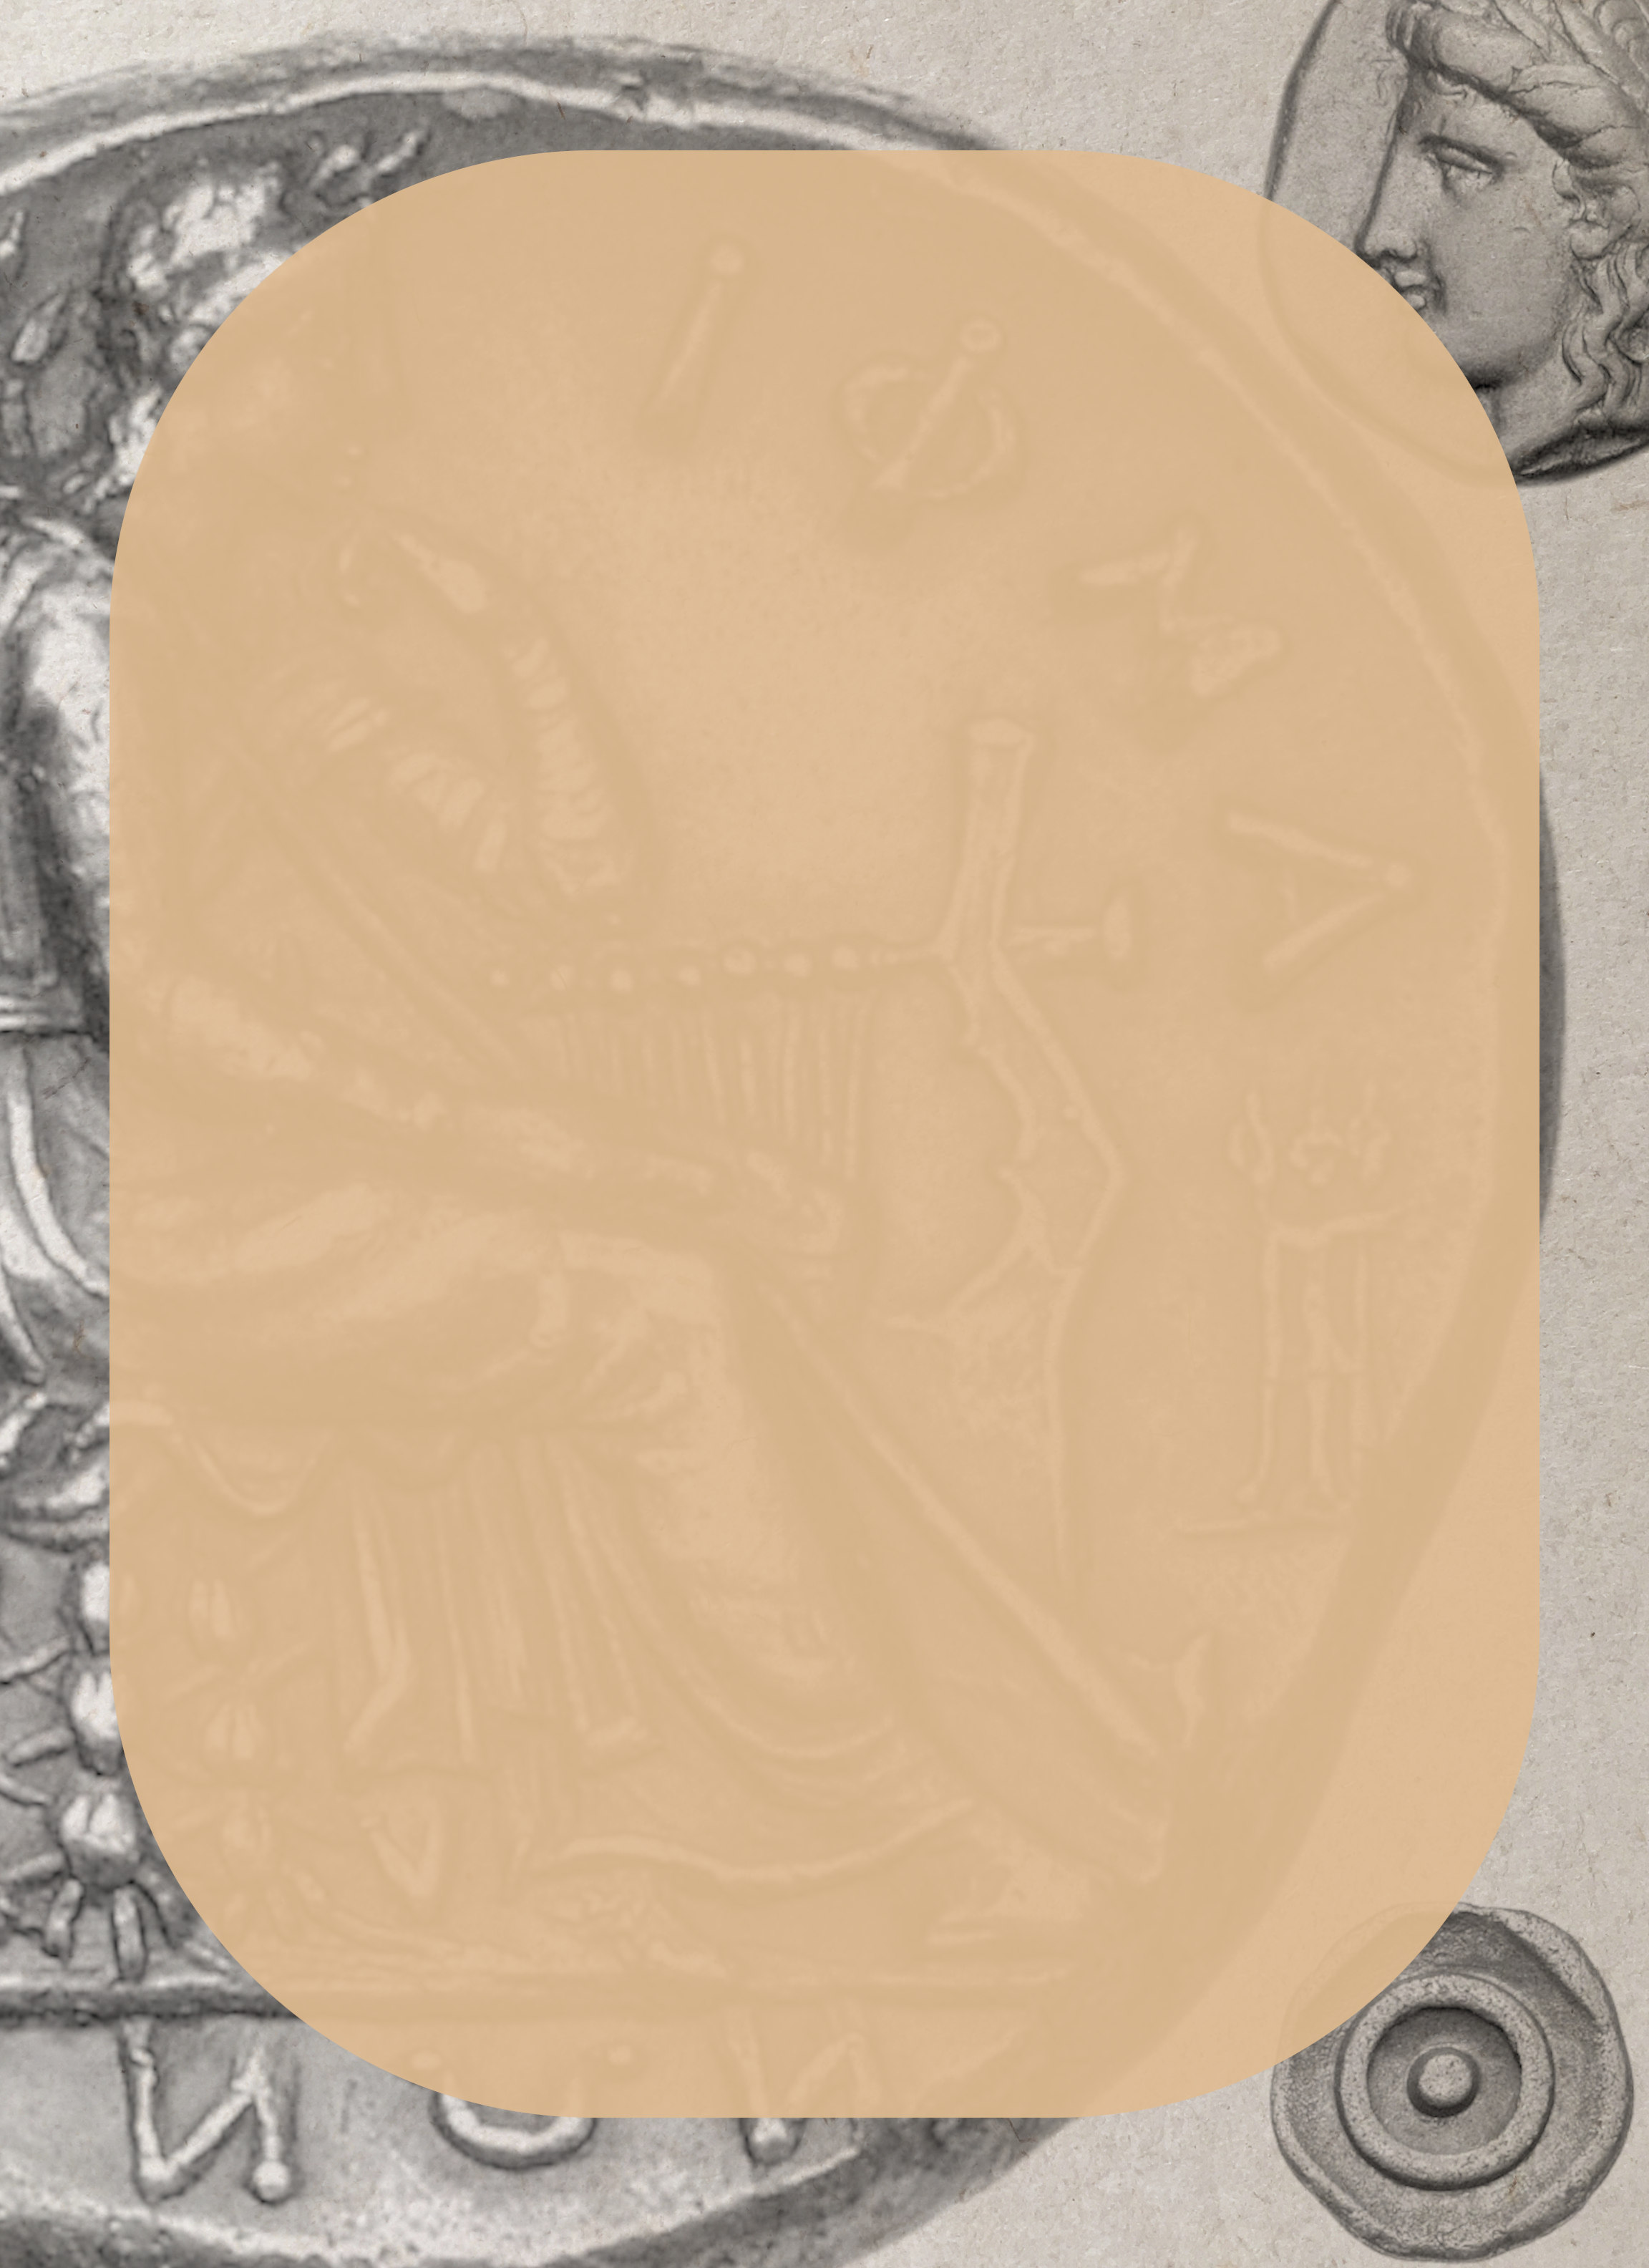
\includegraphics[width=\paperwidth,height=\paperheight]{Hemp_paper_in_Japan-omphalos.jpeg}}

\renewcommand\thefootnote{{\bfseries\color{BrickRed}{\arabic{footnote}}}}
\let\oldfootnote\footnote
    \renewcommand{\footnote}[1]{\oldfootnote{{\normalsize\bfseries\color{BrickRed}#1}}}
\begin{titlepage} % Suppresses headers and footers on the title page
	\centering % Centre everything on the title page
	%\scshape % Use small caps for all text on the title page

	%------------------------------------------------
	%	Title
	%------------------------------------------------
	
	\rule{\textwidth}{1.6pt}\vspace*{-\baselineskip}\vspace*{2pt} % Thick horizontal rule
	\rule{\textwidth}{0.4pt} % Thin horizontal rule
	
	\vspace{1\baselineskip} % Whitespace above the title
	
	{\scshape\Huge Neue Omphalosstudien}
	
	\vspace{1\baselineskip} % Whitespace above the title

	\rule{\textwidth}{0.4pt}\vspace*{-\baselineskip}\vspace{3.2pt} % Thin horizontal rule
	\rule{\textwidth}{1.6pt} % Thick horizontal rule
	
	\vspace{1\baselineskip} % Whitespace after the title block
	
	%------------------------------------------------
	%	Subtitle
	%------------------------------------------------
	
	{\scshape Ein Archäologischer Beitrag zur vergleichenden Religions-Wissenschaft} % Subtitle or further description
	
	\vspace*{1\baselineskip} % Whitespace under the subtitle

        {\scshape Von \Large Dr. Wilhelm Heinrich Roscher}

	\vspace*{2\baselineskip} % Whitespace under the subtitle

        {\scshape\small Mit 58 Figuren auf 7 Tafeln und drei Bildern im Text}

	\vspace{1\baselineskip}

        %------------------------------------------------
	%	Editor(s)
	%------------------------------------------------
        \vspace*{\fill}

        \begin{figure}[H]
        \centering
        \includegraphics[width=0.55\textwidth,keepaspectratio]{figures/transparent/rosher-omph2-tab5-2.png}
        \end{figure}

	\vspace{1\baselineskip}

        \vspace*{\fill}

	{\small\scshape Leipzig 1915}
	
	{\small\scshape{Bei B. G. Teubner}}
 
	\vspace{0.5\baselineskip} % Whitespace after the title block

        \scshape Internet Archive Online Edition  % Publication year
	
	{\scshape\small Namensnennung Nicht-kommerziell Weitergabe unter gleichen Bedingungen 4.0 International} % Publisher
\end{titlepage}
\setlength{\parskip}{1mm plus1mm minus1mm}
\clearpage
\Large
\tableofcontents
\clearpage
\section*{Register --- Systematische Inhaltsübersicht.}
\subsection*{Vorwort.}
\subsection*{Kap. 1: Über die Etymologie von ὀμφαλός (= \emph{umbilicus} etc.) und die Bedeutung des `Nabels' bei den Griechen und andern Völkern:}
\paragraph{}
Meringers neue Etymologie von Wu. \emph{nebh} = `bewässern,' `benetzen,' wonach ὀμφ. (= umbilicus) eigentlich nicht den `Nabel,' sondern die (den Embryo `wässernde') `Nabelschnur' bedeuten soll: S. 5-10. --- Widerlegung dieser Ansicht und Nachweis, dass in den verschiedensten Sprachen das Wort für `Nabel' ursprünglich die Vertiefung in der Mitte des Leibes und folglich `Zentrum' und erst in zweiter Linie die `Nabelschnur' bedeutet: S. 6-8. --- Die neuen von Meringer nachgewiesenen, an die Nabelschnur geknüpften Vorstellungen und Gebräuche verschiedener Völker: S. 8-10. --- Der Nabel als Sitz der Seele und Ausgangspunkt bei der Bildung des Embryos im Mutterleibe; die merkwürdige, bisher noch unerklärte Sekte der Ὀμφαλόψυχοι auf dem Athos: S. 11 f.

\subsection*{Kap. 2: Der Gedanke eines Zentrums (`Nabels') der Erdoberfläche bei verschiedenen Völkern.}
\paragraph{}
Dschedda am Roten Meere, das Grab Evas und `Nabel der Welt' Hach arabischer Auffassung: S.13f. --- Die Vorstellungen der Inder und Phönizier: S. 14 f. --- Neue Zeugnisse für die Geltung Jerusalems als `Nabel der Welt': S. 15-18 (u. 73 f.). --- Vielleicht wurde auch das im Zentrum d. Peloponnes gelegene Lykaiongebirge als `Nabel d. Erde' angesehen: S. 19-22. --- Die Annahme von Svoronos, dass ein in der Mitte der athenischen Akropolis gelegenes Heiligtum der Ge zugleich als ὀμφαλὸς γῆς angesehen worden sei: S. 22-23. --- Die von J. Loth entdeckten Zeugnisse für die Annahme eines `Nabels der Erde' im Gebiete der Kelten: S. 24 ff.

\subsection*{Kap. 3: Branchidai (Didyma) und sein Orakel als Nabel der Erde:}
\paragraph{}
Für meine Annahme, dass Ionien und Milet (Branchidai) in älterer Zeit neben Delphi als Mittelpunkt der Erdscheibe gegolten habe und deshalb auf der ältesten Weltkarte der Ionier als deren Zentrum dargestellt worden sei, spricht jetzt auch die von Jacoby, unabhängig von mir, ausgesprochene Ansicht, dass die ältesten ionischen Geographen nach Herod. 1, 142 etc. nicht Delphi, sondern Ionien wegen seines mittleren Klimas für das Zentrum der Erde gehalten und als solches dargestellt hätten: S. 29 f. --- Neues Relief von Milet mit der Darstellung eines ruhenden Apollon, der einen schlangenumwundenen Omphalos neben sich hat: S. 30.

\subsection*{Kap. 4: Delphi und sein Orakel als Mittelpunkt (ὀμφαλός) der Welt und sein Nabelstein.}
\subsubsection*{A. Die literarischen Zeugnisse.}
\paragraph{}
Über die Frage, ob es im Adyton zu Delphi ein χάσμα (στόμιον) γῆς gegeben hat oder nicht: S. 31-41. --- Die antiken Zeugnisse des Aischylos, Cicero, Strabon, Diodor, Pompejus Trogus, Apollodor, Ps.-Aristoteles (de mundo), Plinius, Plutarch, Cassius Dio, Pausanias: S. 31-37. --- Die neueren Zeugnisse Pomtows, Karos und Baedekers: S. 38 ff. --- Ergebnis: auf Grund der Schriftstellerzeugnisse kann an der einstigen Existenz eines χάσμα γῆς und einer damit in Verbindung stehenden Quellader der Kassotis im Adyton kaum gezweifelt werden: S. 40 f. --- Nach Pomtows Ansicht wird das χάσμα selbst oder wenigstens seine Stelle sicher aufgefunden werden, sobald man --- was bis 1912 noch nicht geschehen war --- das Adyton sorgfältig ausgräbt: S. 39 ff. --- Der ursprüngliche alte Omphalos muss im Adyton in unmittelbarer Nähe des χάσμα und des pythischen Dreifußes gestanden haben, aber außerdem gab es wahrscheinlich noch einen zweiten Omphalos in der eigentlichen Tempelcella, der in einer besonderen `aedicula' stand und im Gegensatz zu dem alten Nabelstein des nur wenigen zugänglichen Adytons für alle Tempelbesucher sichtbar und zugänglich war: S. 42 f. --- Wie es scheint, ist es jetzt dem französischen Archäologen Courby gelungen, den echten alten Nabelstein des Adytons aufzufinden: S. 43 ff. --- Über Varro de l. l. 7, 17: S. 46. --- Über den ὀμφαλὸς γᾶς im Tempel des Apollon Pythaeus in Argos: S. 46 f. --- Weitere Schriftstellerzeugnisse für Delphi als `Nabel der Erde': S. 47 f.

\subsubsection*{B. Die monumentalen Zeugnisse.}
\paragraph{}
a. Die plastischen Nachbildungen des delphischen Omphalos.

Der von Rhomaios entdeckte Omphalos von Thermos in Aitolien: S. 49 f. --- Der Marmoromphalos von Delos: S. 50 f. --- Das Omphalosrelief von Kyzikos: S. 51 f. --- Die Kandelaberbasis aus den Thermen des Titus: S. 52. --- Das aus dem Temenos des Apollon Daphnephoros zu Eretria stammende Omphalosrelief etc.: S. 52 f.

b. Wandgemälde.

c. Der delphische Omphalos auf Münzen.

d. Vasenbilder.

\subsection*{Kap. 5: Weitere wahrscheinlich nicht von Delphi abhängige Kulte des Apollon, Asklepios usw., in denen Omphaloi vorkamen.}
\paragraph{}
Der omphalosförmige `Bomos' im Tempel zu Thymbra: S. 58 f. --- Die Kulte von Patara und Lyrbe: S. 59. --- Der Omphalos als Attribut des Telesphoros und der Hestia: S. 59 f.

\subsection*{Kap. 6: Grabmonumente in Omphalosform.}

\subsection*{Kap. 7: Problematische Omphaloi.}
\paragraph{}
Der netzbedeckte, schlangenumwundene Omphalos' in mehreren umgedeuteten Reliefs etruskischer Aschenkisten: 8. 62---64. --- Verschiedene `Omphaloi' (Baityloi?) auf Münzen und Tesseren: S. 64ff. --- Die von Bulard als Symbole der Hestia und des Genius gedeuteten (gemalten) Omphaloi, an den Außenwänden von Häusern auf Delos: S.67 ff. --- Omphaloi(?) auf attischen Bleitesseren: 8. 69.

\subsection*{Schlusswort.}

\subsection*{Zusätze und Berichtigungen.}

\subsection*{Systematische Inhaltsübersicht.}

\subsection*{Alphabetisches Register.}

\subsection*{Stellenregister.}

\subsection*{Erläuterndes Verzeichnis der Abbildungen.}

\subsection*{Postskripta.}
\clearpage
\begin{quotation}
\normalsize
\begin{flushright}
Οὔτε γὰρ ἦν γαίης μέσος ὀμφαλὸς οὔτε θαλάσσης·

Εἰ δέ τίς ἐστι, θεοῖς δῆλος, θνητοῖσι δ᾽ ἄφαντος.\hspace*{1em}

Epimenides.
\end{flushright}
\end{quotation}
\section*{Vorwort.}
\paragraph{}
`Dies diem docet': die Wahrheit dieses Spruches hat sich auch bei dem von mir kürzlich behandelten Omphalosproblem bewährt; denn bereits in den wenigen Monaten, die seit dem Erscheinen meines `Omphalos'\footnote{Omphalos. Eine philologisch-archäologisch-volkskundliche Abhandlung über die Vorstellungen der Griechen und anderer Völker vom `Nabel der Erde' [29. Bd. d. Abhandl. d. kgl. sächs. Ges. d. Wiss. mit 68 Figuren auf 9 Tafeln und 3 Bildern im Text]. Leipz. 1913, B. G. Teubner.} verstrichen sind, haben sich mir so zahlreiche Nachträge zu dem dort gesammelten und verarbeiteten Material ergeben, dass ich es schon jetzt wohl wagen darf, diese zur weiteren Förderung des genannten Problems herauszugeben. Ganz besondere Anregung in dieser Hinsicht verdanke ich --- abgesehen von der dem französischen Archäologen Courby kürzlich gelungenen Wiederentdeckung des echten alten Nabelsteins im Adyton des delphischen Apollontempels (s. unt. S. 44 ff.) und der Rhomaios verdankten Skizze und Beschreibung des merkwürdigen Omphalos von Thermos (S. 49 f.), sowie von mehreren, bisher noch nicht von mir berücksichtigten Monumenten und Zeugnissen\footnote{Dazu rechne ich mit in erster Linie die von dem bekannten französischen Keltologen J. Loth kürzlich entdeckten Zeugnisse für die einstige Existenz der Omphalosidee auch bei den Kelten (s. unten 9. 24 f.).} --- dem ebenso gelehrten wie scharfsinnigen Aufsätze Rud. Meringers, der fast gleichzeitig mit meinem `Omphalos,' und also völlig unabhängig von diesem, unter dem Titel `Omphalos, Nabel, Nebel' in der Zeitschrift `Wörter und Sachen' (Kulturhistor. Ztschr. f. Sprach- und Sachforschung 5, 1 (1913) S. 43-91) erschienen ist. Wenn ich mich auch im Folgenden mehrfach nicht bloß zustimmend, sondern auch widersprechend und kritisierend mit der genannten Arbeit Meringers zu beschäftigen habe, so möchte ich doch gleich von vornherein dankbar hervorheben, dass m. E. Meringer die gesamte Omphalosfrage durch Sammlung und Verarbeitung eines ganz gewaltigen Materials so vielseitig gefördert hat, dass künftig niemand achtlos an seiner wertvollen Arbeit vorübergehen darf, die bis auf weiteres als die reichhaltigste Ergänzung meines `Omphalos' und zugleich als eine deutliche Bewahrheitung des homerischen σύν τε δύ᾽ ἐρχομένω καί τε πρὸ ὁ τοῦ ἐνόμσεν gelten muss. Ich schließe mich in diesen neuen Omphalosstudien möglichst eng an die Reihenfolge der einzelnen Kapitel meines `Omphalos' an und bemerke nur noch, dass ich diesen im Folgenden einfach mit `O.,' Meringers Abhandlung dagegen mit `M.' zitieren werde.
\clearpage
\section{Kapitel 1}
\begin{center}
\textbf{Über die Etymologie von ὀμφαλός (= \emph{umbilicus} etc.) und die Bedeutung des `Nabels' bei den Griechen und anderen Völkern (vgl. O. S. 6-19 und S. 131 f.).}
\end{center}
\paragraph{}
Während ich es (O. S. 6) dahingestellt sein ließ, ob das indogermanische Urwort für `Nabel' mit G. Curtius und J. Schmidt (M. S. 82 unt.) auf eine Wurzel \emph{nabh} = `bersten, reißen' zurückzuführen sei, und ursprünglich `Riss, Bruch' bedeutet habe, will Meringer (S. 82 ff.) lieber von der Wurzel *\emph{enebh} = `bewässern,' `benetzen,' `befeuchten' ausgehen,\footnote{Vgl. ai. \emph{nabhrāj}, avest. \emph{nab} = befeuchten, ai. \emph{ámbhas} = Wasser, ai. \emph{nábhas} = Nass, Nebel, Wolke (= νέφος) etc.: M. 83 f.} indem er annimmt, dass der Ursinn von `\emph{Nabel},' ὀμφαλός etc. nicht `Nabel' (d. i. die in der Mittellinie des Leibes nach dem Abschneiden des funiculus umbilicalis zurückgebliebene, meist eine Vertiefung darstellende Narbe), sondern vielmehr `Nabelschnur' gewesen sei, die er richtig als das dem Embryon das Blut zuführende und es auf diese Weise ernährende Organ auffasst (vgl. M. S. 43 f. und O. S. 6 f. Anm. 6). Ob diese lautlich, wie mir scheint, vollkommen genügend begründete Ansicht M.s auch logisch und sachlich als einwandfrei betrachtet werden kann, ist mir freilich einigermaßen zweifelhaft geworden auf Grund folgender Erwägungen.

a. Der z. B. im Griechischen, Lateinischen und Deutschen bei weitem überwiegende Sprachgebrauch beweist deutlich, dass man unter ὀμφαλός, \emph{umbilicus}, `Nabel' ursprünglich und hauptsächlich nicht die nur kurze Zeit während der Entbindung sichtbare Nabelschnur, sondern vielmehr die bei allen lebenden und toten Menschen und Säugetieren dauernd sichtbare rundliche Vertiefung in der Mittellinie des Leibes verstanden hat.

b. Wenn bisweilen, aber im ganzen doch ziemlich selten,\footnote{Das erkennt auch M. selbst S. 50 an, wenn er ausdrücklich sagt: `Ich kenne nur zwei Stellen, in denen das Wort (ὀμφαλός) diesen Sinn (`Nabelschnur') hat': Demokr. b. Diels, Fragm. d. Vorsokrat.* 1 S. 411 und Poll. on. 2 223. Bei Soranos, Gynaec. ed. Rose S. 250, 2 heißt sie nicht ὀμφαλός, sondern ὀμφαλίς, im Gegensatz zu jenem (p. 250, 22).} in den genannten Sprachen, wie wohl auch in den meisten andern, unter ὀμφαλός, \emph{umbilicus} usw. auch die Nabelschnur zu verstehen ist, so ist diese Bedeutung, wie auch, so viel ich sehe, alle Lexikographen anerkennen, nicht als die ursprüngliche, sondern schon als eine sekundäre (übertragene) anzusehen, die gegenüber der viel gewöhnlicheren und ursprünglicheren (= \emph{Nabel}) kaum sonderlich in Betracht kommen kann.

c. So erklärt sich auch am einfachsten die von Meringer (und ebenso von Nilsson in seiner sonst sehr dankenswerten Anzeige meines `Omphalos' in der D. Lit. Ztg. 1914 Nr. 6 S. 332 ff.)\footnote{Ich kann also Nilsson a. a. O. Sp. 333 durchaus nicht beistimmen, wenn er meint, `ὀμφαλός könne jeden rundlichen, aufgehöhten Gegenstand ohne Beziehung auf eine Lage in der Mitte bezeichnen,' und sich dafür auf die Tatsache beruft, dass nach einigen Stellen bei Homer auch Schilde mit mehreren ὀμφαλοί vorkommen. Denn auch in diesem Falle befindet sich der eigentlichste und wichtigste ὀ. natürlich genau in der Mitte und ist symmetrisch von mehreren Nebenbuckeln unweit des Randes umgeben, deren jeder wieder das Zentrum einer kleineren Fläche am Rande bezeichnet. Denn es ist doch im höchsten Grade unwahrscheinlich, dass die Randbuckel ganz willkürlich und unsymmetrisch angebracht gewesen seien.} nicht genug gewürdigte Tatsache, dass in allen mir bekannten Sprachen das Wort für `Nabel' schon seit ältester Zeit viel häufiger in der offenbar uralten übertragenen Bedeutung `Mittelpunkt,' `Zentrum' als im Sinne von Nabelschnur vorkommt, welche Übertragung sich logisch zweifellos sehr viel leichter aus dem Begriffe des `Nabels' als aus dem des `Nabelstrangs' erklären lässt. In dieser Hinsicht verweise ich nicht bloß auf die sämtlichen indogermanischen Sprachen, in denen der Ausdruck für `Nabel' zugleich `Mittelpunkt,' `Zentrum' bedeutet,\footnote{Vgl. hinsichtlich des Sanskrit meine Darlegungen O. S. 19 A. 33 u. S. 22; im übrigen verweise ich auf die deutschen Wörterbücher von Grimm und Sanders unter `\emph{Nabel},' auf die spanischen Lexika unter \emph{ombligo}, auf die italienischen unter \emph{ombellico, umbilico, bellico}, auf die französischen unter \emph{nombril} und \emph{ombilic} usw. Vgl. auch Gruppe i. d. Berl. Philol. Wochenschr. 1913, Sp. 434 a Meltzer, Philol. 1904, S. 198. Blümner in d. Berl. Philol. Wochenschr. 1914, Sp. 1525.} sondern ebenso auch auf die semitischen\footnote{S. O. S. 24 A. 43. S. 25 A. 44 u. 45. S. 26 A. 47. S. 28. Vgl. auch Rhodokanakis in `Wörter u. Sachen' Bd. 5 Heft 2 (1913) S. 199 Anm. 9 f. S. 201 u. 202.} und deren Dialekte, ferner auf das Türkische,\footnote{S. O. S. 28 A. 52.} das Malaysische\footnote{S. O. S. 22 nr. 3.} und sogar das Peruanische,\footnote{S. O. S. 35 nr. 13.} deren Übereinstimmung in diesem wichtigen Punkte ebenso auf das hohe Alter wie auf die Ursprünglichkeit und Natürlichkeit der zugrunde liegenden Metapher hindeutet. Auch beweisen die zahlreichen teils von Meringer teils von mir (O. S. 8 ff.) gesammelten Zeugnisse für den Gebrauch von ὀμφαλός, \emph{umbilicus, Nabel} zur Bezeichnung der nabelförmigen Erhöhung (bez. Vertiefung) in der Mitte der φιάλαι (ὀμφαλωταί),\footnote{O. S. 96; M. S. 57. f.} oder des in der Mitte der Sonnenuhren angebrachten Zeigers (γνώμων),\footnote{M. S. 62 mit Abbildung.} oder des stets in der Mitte des Waagebalkens angebrachten `Züngleins' der Wage,\footnote{M. S. 62.} oder des Mittelpunkts der antiken Windrosen,\footnote{O. S. 45 f. (Plin. h. n. 18, 326 ff.). M. S. 63 f.} oder endlich des stets in der Mitte der Oberseite der liegenden (zur Ausbrütung bestimmten) Eier befindlichen `Hahnentritts'\footnote{M. S. 63 (Plin. h. n. 10, 145) und dazu Brockhaus, Konvers.-Lex. 14 unter Ei (Tafel, Abb. 1).} usw.,\footnote{Über die ὀμφαλοί der Buchrollen s. jetzt auch M. S. 51 f. mit Abbildungen (sowie Hugo Blümner in der Berliner Philolog. Wochenschr. v. 28./11. 1914 Sp. 1525), über den `Nabel' des homerischen Maultierjochs (Il. Ω 273) ebenda S. 53 ff. (mit Abbildungen). Vgl. auch O. S. 8 ff.; über ὀ. als zentralen Schlussstein eines Gewölbes vgl. M. S. 61 oben und O. S. 9 A. 12. --- Auch bei der als ὀμφαλὸς θαλάσσης gedachten Kalypsoinsel (Odyss. α 50) handelt es sich, wie man aus Epimenides fr. 1 Ki. = Plut. Mor. S. 409 E. deutlich erkennt, unzweifelhaft um die Mitte des Meeres, und ich verstehe nicht recht, wie M. a. a. O. S. 57 behaupten kann, `hier liege ein anderes Bild vor: Das Eiland erhebe sich rund aus dem Meere wie der Nabel aus dem Unterleibe.' Dieser Deutung widerspricht schon die von M. selbst S. 44 f. und 65 richtig hervorgehobene Tatsache, dass der `krankhaft hervorgetriebene Nabel' nie der Nabel, nie der `normale Nabel' gewesen ist.} wie klar und deutlich überall bei den Wörtern mit der Bedeutung `Nabel' das Merkmal der zentralen Lage oder Stellung hervortritt. Sogar in dem (O. S. 12 Anm. 21) einzigen bisher von mir notierten Falle, wo ὀμφαλός nicht die genaue Mitte zu bezeichnen scheint, nämlich in der siebenfachen Gliederung des Terpandrischen νόμος κιθαρῳδικός bei Pollux On. 4, 66, wo ὀμφαλός nicht an 4., sondern an 5. Stelle steht, `ist entweder mit Westphal durch Umstellung oder aber durch Ausscheidung der μεταρχά und μετακατατροπά aus einem älteren Schema zu helfen' (Drerup im Lit. Zentralbl. 1913 Sp. 1774).\footnote{In einem Brief vom 19./11. 13 bemerkte mir Drerup: `Der ὀμφαλός des νόμος κιθαρῳδικός ist doch der Mitte sehr nahe: ἀρχά und μεταρχά κατατροπά und μετα κατατροπά führen auf eine ursprünglich einfachere Form des νόμος; sicher: ἀρχά (μεταρχά), κατατροπά (μετα κατατροπά), ὀμφαλὸς, σφραγίς, ἐπίλογος, wodurch ὀμφ. genau in die Mitte gerät.'} Übrigens gilt fast dasselbe auch von den nicht seltenen Fällen, dass bei der Bezeichnung gewisser Pflanzenteile, z. B. des Stieles der Baumfrüchte oder des aus dem Kerne (Samen) der Pflanzen hervorsprießenden Keimes, als ὀμφαλός (O. S. 8 Anm. 9 und 11; M. S. 52) an das Bild der Nabelschnur zu denken ist; denn wie ich (O. S. 8) nachgewiesen habe, handelt es sich auch hier durchweg um Begriffe, zu deren Hauptmerkmalen eben das der zentralen Lage in der Mittellinie (Achse) der Frucht oder des Kernes gehört.

Wenn ich also (O. S. 19)\footnote{Vgl. auch a. a. O. S. 12.} als das vornehmste der durch meine Erörterungen erzielten Ergebnisse die zentrale Lage oder Stellung aller mit ὀμφαλός und \emph{umbilicus} bezeichneten Begriffe innerhalb eines größeren Ganzen hingestellt habe, so ist dieses Resultat bis jetzt noch in keiner Weise erschüttert oder gar widerlegt worden.

Je weniger ich aber in diesem Punkte Meringer beizustimmen vermag, um so freudiger begrüße ich seine mit den meinigen vollkommen harmonierenden und dieselben in höchst wertvoller Weise ergänzenden Darlegungen hinsichtlich der bei den meisten Natur- und Kulturvölkern üblichen Behandlung und Aufbewahrung der abgeschnittenen Nabelschnur\footnote{S. M. S. 45 ff. u. 77 ff. Besonders beachtenswert erscheint die von Meringer S. 47 Anm. 1 (unter Verweisung auf Jolly, Medizin, Grundr. d. indoarischen Philol. u. Altertumskunde 3, 10 S. 58; Avicenna, Lib. can. de medic. Venet. 1582 S. 56 H.; T. Bellini s. v. belliconchio) angeführte Tatsache, dass die Nabelschnur des Embryo 4 Fingerbreiten weit vom Nabel abgeschnitten werden soll. Das entspricht genau dem altgriechischen von Soranos bezeugten Brauche (s. O. S. 7 Anm. 8).} (s. O. S. 12 ff. u. S. 131 f.). Als besonders interessante, von mir bisher übersehene, abergläubische, den aufbewahrten Nabelschnurrest betreffende Gebräuche und Anschauungen trage ich aus Meringers Sammlungen hier folgendes nach.

M. S. 46 f.: `Nach R. Andree, Braunschweiger Volkskunde 2 S. 289 wurde ein Teil der Nabelschnur des Kindes mit einem seidenen Bändchen versehen, darauf der Name des Kindes geschrieben und so dem Gevatter als Einladung übergeben, der damit gleichsam einen Teil des Kindes zum Eigentum erhielt, symbolische Andeutung der engen [geistigen oder seelischen] Beziehung zwischen dem Gevatter und seinem Patenkinde.'

`Eine eigene Bedeutung legt der Aberglaube dem Bändchen bei, mit dem der Nabel abgebunden wurde, das aber bei dem Nabelschnurreste bleibt.\footnote{Vgl. dazu die bei Meringer S. 79 gegebenen Abbildungen solcher getrockneten Nabelschnüre mit Bändern, aus deren Form er freilich wunderlicherweise die Gestalt des mit Tainien oder einem Bindennetze geschmückten ὀμφαλός γῆς von Delphi ableiten will. S. dagegen Nilsson, D. Lit. Ztg. 1914 Nr. 6 Sp. 335 f.} Wenn das Kind später\footnote{D. h. in der Regel in seinem 7. Lebensjahre, in dem die Verstandesreife und damit der Unterricht des Kindes beginnt (s. unt. u. vgl. Roscher, D. ennead. u. hebdomad. Fristen u. Wochen d. ältesten Griechen S. 33 f. Anm. 114. S. 64 Anm. 187. Ders., Hebdomadenlehren S. 13 f. Anm. 12. S. 27 Anm. 33. S. 105 Anm. 165).} den Knoten lösen kann, wird es geschickt und reich werden (vgl. v. Hovorka-Kronfeld, Vergleich. Volksmedizin 2 S. 636). Solche Vorstellungen sind bezeugt aus Ostpreußen, dem Frankenwalde und der Schweiz. Sie finden sich auch, wie ich höre, in Mähren und sind wahrscheinlich noch viel weiterverbreitet.' `Von einem Menschen, der sich geistig zu seinem Vorteil verändert hat, sagt man, der Knopf\footnote{Dass hier unter `Knopf' eigentlich der Nabel zu verstehen ist, scheint mir auch hervorzugehen aus der Bezeichnung des Nabels als `Bauchknöpfchen' z. B. in der Gegend von Leipzig.} sei ihm endlich aufgegangen. Bei Kindern hofft man auf das Aufgehen des Knopfes, d. h. auf das Erwachen des Verstandes. Mich dünkt es für geraten, anzunehmen, dass diese Redensarten mit dem eben berichteten Brauche zusammenhängen, denn der, dem der Knopf aufgeht, ist geistig begabt. In der Schweiz sagt man von einem jungen Menschen, der plötzlich zu wachsen beginnt: er tut den Knopf auf (D. Wb. 5 Sp. 1477).'\footnote{Freilich könnte `Knopf' in diesen Fällen vielleicht auch so viel als `Kopf' sein!} `Alois John, Sitte, Brauch und Volksglaube im deutschen Westböhmen, berichtet: Auch die Nabelschnur wird dem Kinde für später, wenn es erwachsen ist, aufgehoben... Knaben wird sie, wenn der Schulbesuch beginnt [also im 7. Jahre!] zum Aufknoten gegeben. Gelingt ihm dies, so wird er sehr gut lernen.' S. 49: `G. B. Corsi: Vita Senese (Archivio 9 S. 109): `Chi brama di avere un figliolo cantante? Ecco la ricetta. Appena nasce, si piglia un pezzetto del suo cordone ombellicale, si mette su un testucchio o su d'un olmo, e se vi posa qualche usignolo a rallegrare i dintorni delle sue melodie, la grazia è bell' e ottenuta.'\footnote{Hierher gehören auch die Auffassungen des Nabels, die M. S. 66 aus Frankreich und Italien anführt. Vgl. Migne, Dict. d. superstitions unt. `naissance': `A Fresse, près de Ramonchamp, on dit que des femmes qui viennent d'accoucher conservent soigneusement dans une boîte une partie du cordon ombilical. Quand l'enfant est capable de s'exprimer d'une manière intelligible, la mère lui présente ce cordon ombilical. Si l'enfant devine ce que c'est, il est certain, qu'il deviendra un ouvrier très habile et très intelligent.' Im Italienischen bedeutet (nach Petrocchi, Novo Dizion. s. v. bellico) `Tu non ai bellico' so viel als tu non ai giudizio, und man sagt von dem, der keinen Verstand hat `aver l'osso nel bellico.' Vgl. auch die Redensart `Che mi caschi il bellico, se'... = Da könnte man gleich den Verstand verlieren, wenn...}

Wenn M. (S. 49) aus diesen und ähnlichen Zeugnissen den Schluss zieht, dass zwischen Nabelschnur [Nabel] und Verstand [Seele] besondere Beziehungen bestehen, so kann ich unter Verweisung auf die von mir (O. S. 12 ff. u. 131) mitgeteilten Zeugnisse aus dem Bereiche der verschiedensten Völker diese Annahme nur völlig gerechtfertigt finden. Ja ich glaube, wie ich O. S. 12 getan habe, noch einen Schritt weiter gehen und geradezu behaupten zu dürfen, dass wie das in der Mitte des inneren Leibes befindliche Zwerchfell so auch der das äußere Zentrum des Körpers bezeichnende Nabel als Sitz der Seele und des Verstandes aufgefasst worden sein muss,\footnote{Eine weitere ebenfalls wohl sehr alte Vorstellung von der Bedeutung des Nabels findet sich bei Vindicianus cap. 16 = Wellmann, Fragm. d. griech. Ärzte 1, 218 f.: primo mense iactus seminis nostri in utero materno congregatur in umbilicum, in hoc est congregatio etc. Vgl. dazu Hipp. π. φυς. παιδ. 15 = 7 492 L. Democr. b. Plut. de am. prol. c. 3; vgl. Censorin. d. n. 6, 1. Diels 190. `Diese Annahme beruht auf pythagoreischer Doktrin: vgl. Philolaus b. Jambl. theol. ar. S. 22' (Wellm.). Übrigens findet sich eine ganz ähnliche Anschauung bei den Israeliten, denn im Midrasch der Göttlichen Weisheit (Jellinek, Beth ha-Midr. 5, 65) heißt es: "`Gott gründete mit Weisheit die Erde."' Gott erschuf die Welt wie das vom Weibe Geborene. So wie dieses vom Nabel aus sich entwickelt, so begann Gott die Welt vom Nabel [aus] zu erschaffen, woher sie sich dann weiterentwickelte. Wo ist der Nabel? Das ist Jerusalem. Der Nabel selbst ist der Altar. Und warum heißt er (der Altar) Stein schethijja? Weil von ihm aus die ganze Welt gegründet wurde."' Feuchtwang, Monatsschr. f. Gesch. u. Wissensch. d. Judent. 1910 S. 727 f. Vgl. auch unt. S. 15 ff.} und dass mit dieser Anschauung eben jene eigentümlichen Beziehungen der Nabelschnur eng zusammenhängen, die wir soeben dargelegt haben. Am allerdeutlichsten zeigt sich jene Anschauung bekanntlich in den homerischen Gedichten, in denen φρένες, d. i. das in der Mitte der Eingeweide und in der Nähe des Nabels liegende Zwerchfell, durchaus als Sitz der Seele und der Denkkraft erscheint, sodann in der Bezeichnung einer bestimmten mit Verwirrung des Verstandes verbundenen Krankheit, der sogen. φρενῖτις, als deren Sitz offenbar das Zwerchfell betrachtet wurde.\footnote{Vgl. Roscher, Üb. Alter, Ursprung u. Bedeutung d. hippokr. Schr. v. d. Siebenzahl S. 16 A. 21 f. und Omphalos S. 12 Anm. 20.} Auf demselben altertümlichen Standpunkte stehen auch noch der Kosmologe und der Pathologe der hippokratischen Schrift π. ἑβδομάδων, wenn ersterer in Kap. 11 das in der Mitte zwischen dem kalten Norden und dem heißen Süden gelegene und durch die hohe Kultur und Intelligenz seiner Bewohner ausgezeichnete Ionien das `Zwerchfell der Erde' nennt, und letzterer in Kap. 52 geradezu den Sitz der Seele (ψυχή) in der Gegend des Nabels und des Zwerchfells behauptet.\footnote{Roscher a. a. O. und in der Ausgabe der Schrift π. ἑβδ. S. 16. S. 79. S. 142 f. S. 153. S. 157.} In der Folgezeit wurde diese uralte und volkstümliche Anschauung von dem Sitze der Seele in der Nabelgegend in den Kreisen der Gebildeten freilich durch die von Hippokrates und den meisten Philosophen vertretene Theorie von dem Sitze der Seele und des Verstandes im Gehirn fast völlig verdrängt; dass sie aber doch auf griechischem Boden niemals ganz erstorben ist, scheint nicht bloß aus den oben berührten noch heute in Hellas bestehenden abergläubischen Riten und Anschauungen hervorzugehen, sondern wird auch durch die eigentümliche in den Athosklöstern des 14. Jahrh. heimische Sekte der Ὀμφαλόψυχοι ausdrücklich bestätigt. Wie schon der Name lehrt, der geradezu `Nabelseelen' bedeutet, gingen die Anhänger dieser Richtung von der Annahme aus, dass als Sitz der Seele der Nabel als Mittelpunkt des Körpers anzusehen sei, und gründeten auf diese Lehre einen eigentümlichen, ihre innere Förderung und Erleuchtung bezweckenden Ritus. Dieser bestand darin, dass sich der Ὀμφαλόψυχος bei verschlossener Tür ganz allein in einen Winkel seiner Zelle setzte und, um sein Gemüt von allem Irdischen und Vergänglichen abzuziehen, selbst den Atem möglichst zurückzuhalten versuchte, vor allem aber das Kinn auf die Brust legte und dabei die Augen unverwandt auf die Mitte des Bauches, d. h. den Nabel, richtete. Auf solche Weise glaubte man (offenbar eingedenk des Spruches Γνῶθι σεαυτόν) in das Innere des eigentlichen Ichs, den Sitz aller Seelenkräfte, einzudringen und einer wunderbaren Erleuchtung teilhaftig zu werden. Man behauptete, die Wirkung dieses Ritus sei anfangs, dass der Gläubige sich von einer dichten Finsternis umgeben fühle; beharre man aber so ununterbrochen Tag und Nacht und gelinge es dem Verstande, den Ort des Herzens (= Nabels?) d. i. der Seele zu erschauen, so sehe man dann alles, was vorher dunkel war; ein höheres Licht dringe hervor, in ihm sehe man sich selbst, in seinem wahren von allem Irdischen losgetrennten Wesen, und von überschwänglicher Seligkeit fühle man sich durchdrungen.\footnote{Vgl. außer den Konversationslexika von Brockhaus und Meyer unter `Hesychasten' auch Ersch und Grubers Enzyklopädie unter demselben Wort und Ph. Meyer in der Realencyclop. f. protest. Theol. u. Kirche 3 Bd. 8.} Auch dieser sonderbare in der griechischen Kirche des 14. Jahrhunderts mit großer Kraft sich durchsetzende Ritus scheint mir unwiderleglich zu beweisen, dass sich der uralte Glaube an den Sitz der Seele im Zentrum des Körpers, d. h. in der Gegend des Nabels und des Zwerchfells, in den Kreisen des naiven griechischen Volkes, allen medizinischen und philosophischen Theorien zum Trotze, bis ins 14. Jahrhundert intakt erhalten hatte, wie er denn auch heute noch in gewissen Bräuchen und Volksanschauungen fortlebt.\footnote{Eine ähnliche Vorstellung liegt wohl auch dem von Sanders im Wörterb. d. deutschen Sprache 2, 1 S. 368 c unter `Nabel' (aus Goethe 12, 293) angeführten Satze zu Grunde: `Im Nabel ist sie [die Seele] gern zu Haus' (`mit Anspielung auf Somnambulismus etc.').}
\clearpage
\section{Kapitel 2}
\begin{center}
\textbf{Der Gedanke eines Zentrums (`Nabels')\footnote{Dieser Mittelpunkt wird geradezu als `Nabel' bezeichnet von den Indern (O. 22), Malayen (O. 22), Israeliten (O. 24 ff.), Arabern und Persern (O. 28 f.), Griechen (O. 32 f.), Italikern (O. 34), Peruanern (O. 35).} der Erdoberfläche bei verschiedenen Völkern.}
\end{center}
\paragraph{}
In dem so überschriebenen zweiten Kapitel des `Omphalos' habe ich den Gedanken des Erdnabels bei Chinesen, Japanern, Malayen, Indern,\footnote{Bei dieser Gelegenheit trage ich nach, dass die moderne Literatur über den `mythischen Berg Meru [= Μηρός der Griechen], den indischen Olymp, der sich nach indischer Auffassung im Zentrum der Erdscheibe zu enormer Höhe erhebt [Himalaya?] und auf dem die Götter wohnhaft gedacht werden,' von W. Fox in der Festschrift für E. Windisch S. 213 Anm. 1 sorgfältig zusammengestellt worden ist.} Babyloniern,\footnote{Zu O. S. 28 ist jetzt noch nachzutragen Jeremias, Handb. d. altorient. Geisteskultur S. 188 a. E., wo die Behauptung ausgesprochen wird, dass Iraq (= Babylonien) oder Iranšahr (Persien) wegen ihrer Lage in der Mitte der 7 (12) Klimata als `Nabel der Welt' aufgefasst worden seien.} Israeliten, Arabern, Persern, Phöniziern,\footnote{Auf das der Astarte von Paphos geheiligte Idol in Gestalt einer `meta' oder eines `ὀμφαλός' (O. S. 29 f.) beziehen sich wohl auch die Worte des Philostratos (v. Ap. Ty. 3, 58): Πάφον, οὗ τὸ τῆς Ἀφροδίτης ἔδος, ὃ ξυμβολικῶς ἰδρυμένον θαυμάσαι τὸν Ἀπολλώνιον, καὶ πολλὰ τοὺς ἱερέας ἐς τὴν ὁσίαν τοῦ ἱεροῦ διδαξάμενον ἐς Ἰωνίαν πλεῦσαι... Bei dieser Gelegenheit werfe ich die Frage auf, ob nicht die beiden Vögel (Tauben?) rechts und links oberhalb des im Tempel von Paphos stehenden `Omphalos' (s. die Münze O. S. 30. ob.) eine gleiche Bedeutung haben, wie die beiden Adler r. u. l. vom delphischen Nabelstein.} Ägyptern,\footnote{Wenn in der (O. S. 31) behandelten Stelle der Κόρη κόσμου des Hermes Trismeg. (Stob. Ecl. 1 S. 302 M.) Ägypten als Zentrum und Herz (καρδία) der Erde bezeichnet wird, so stimmt damit völlig überein Horapollon Hierogl. 1, 7: ἡ καρδία κατ᾿ Αἰγυπτίους ψυχῆς περίβολος und 1, 21: μόνη δὲ ἡ Αἰγυπτίων γῆ, ἐπεὶ μέση τῆς οἰκουμένης ὑπάρχει, καθάπερ ἐν τῷ ὀφθαλμῷ ἡ λεγομένη κόρη. Vgl. auch Horap. 1, 26: τὸ ζῷον [ἡ ἶβις] Ἑρμῇ ὠκείωται, πάσης καρδίας καὶ λογισμοῦ δεσπότῃ... deshalb: καρδίαν βουλόμενοι γράφειν [οἱ Αἰγ.] ἶβιν ζωγραφοῦσι.} Griechen, Italikern, Magyaren und Peruanern verfolgt und nachzuweisen gesucht, dass er überall aus der Vorstellung von einer runden Erdscheibe, die als solche notwendigerweise einen Mittelpunkt (`Nabel') haben musste, erwachsen ist. Ich bin jetzt in der Lage, die Liste der ὀμφαλοὶ γῆς um drei nicht unwichtige Punkte zu vermehren, die mir bisher leider entgangen waren.

Der eine dieser Punkte ist Dschedda, die allbekannte bedeutende Stadt am Roten Meere, der in der islamischen Welt als Sammelplatz für die zur See anlangenden Mekkapilger einen großen Ruf genießende Hafenort für die heiligen Städte des Hedschas. Vor den Mauern dieser Stadt liegt das von den Muhammedanern als Heiligtum ersten Ranges hochverehrte Grab Evas, das geradezu `Nabel der Welt' genannt wird. Ich verdanke den Hinweis auf diese Bedeutung Dscheddas Prof. Rhodokanakis in Graz, der sich in der Zeitschrift `Wörter u. Sachen' (5, 2, 1913 S. 202) auf das Zeugnis Burtons (Pilgrimage 3, 387; vgl. Eisler im Philologus 68, 140) beruft. Dieses lautet: `Whitewashed and conspicuous to the traveller from afar, is a diminutive dome... under it and in the centre is a square stone planted upright and fancifully carved to represent the omphalic region of the human frame. This as well as the dome is called \emph{El Surra} or the navel.' Sicherlich hat diese Bedeutung des ja nicht weit von Mekka gelegenen Dschedda --- auch abgesehen von dem Einflüsse Jerusalems (s. O. S. 29 A. 54) --- wesentlich mit dazu beigetragen, zu verhindern, dass Mekka zum `Nabel der Erde' erhoben wurde, wie Eisler (Weltenmantel u. Himmelszelt S. 723, 1) irrtümlich behauptet (s. dagegen Goldziher Omphalos S. 29).

Hieran reihe ich noch eine kleine Anzahl nachträglicher Bemerkungen zu einzelnen Abschnitten dieses Kapitels.

O. S. 22 habe ich zur Erklärung der Tatsache, dass der religiös begeisterte Inder bei der feierlichen Zeremonie des Opfers wie bei der Aufrichtung der Eckbalken seines Hauses, sich im Mittelpunkt (`Nabel') der Welt zu befinden wähnte, auf den Begriff des Zenits oder Scheitelpunkts verwiesen, worunter allgemein derjenige Punkt am Himmel verstanden wird, der gerade über dem Scheitel des jeweiligen Beobachters steht und zugleich als der mittelste und höchste Punkt des Himmels angesehen wird. Daraus ist mit einer gewissen Notwendigkeit zu schließen, dass in der älteren Zeit, die von der Erdkugel noch keine Ahnung hatte, sondern nur eine runde flache Erdscheibe annahm, im Grunde jeder Punkt auf der Erde den Anspruch erheben durfte, `Nabel der Erde' zu sein, eine Anschauung, die sich ja auch tatsächlich bei den verschiedensten Völkern nachweisen läßt.\footnote{Dass auch den Indern ihr Heimatland als Mitte der Erde erschien, ist mir sehr wahrscheinlich geworden im Hinblick auf Philostratos' (v. Apoll. Ty. 3, 14) Worte: οἱ σοφοὶ, d. h. die Gymnosophisten, φασὶν οἰκεῖν τὰ μέσα τῆς Ἰνδικῆς καὶ τὸν ὄχθον ὀμφαλὸν ποιοῦνται τοῦ λόφου τούτου, πῦρ τε ἐπ᾽ αὐτοῦ ὀργιάζουσιν, ὅ φασιν ἐκ τοῦ ἡλίου ἀκτίνων αὐτοὶ ἕλκειν· τούτῳ καὶ τὸν ὕμνον ἡμέραν πᾶσαν ἐς μεσημβρίαν ᾄδουσιν κ. τ. λ. Wer bedenkt, dass auch sonst vielfach der `Nabel' des Einzellandes mit dem `Nabel der Erde' zusammenfällt, der wird meine Vermutung nicht unwahrscheinlich finden, dass der Wohnsitz der hochgefeierten Weisen im `Nabel' Indiens zugleich den `Nabel der Welt' bedeuten sollte.} So versteht man auch ohne weiteres die altindische Vorstellung, dass Agni und das Opferfeuer der `Nabel der Welt' seien; denn jedes Feuer und jede Opferflamme strebt ja naturgemäß dem Zenit zu, und gerade unter diesem liegt wiederum augenscheinlich der durch den Opferplatz bezeichnete Mittelpunkt der als runde Scheibe gedachten Erde. Übrigens scheint eine ähnliche Vorstellung auch in Babylonien und Phönizien geherrscht zu haben, denn nach A. Jeremias (D. altoriental. Geisteskultur S. 188 ob.) galt bei den Babyloniern `jeder Tempel [mit seinem Opferaltar] im Prinzip als Nabel der Welt,' und Gruppe (Gr. Myth. u. Rel.-Gesch. S. 725, 4) vermutet nicht ohne Wahrscheinlichkeit, dass die Bezeichnung des feurigen Ölbaums in Tyros als ἔρνος πέτρης ὑγροπόροιο μεσόμφαλον (Nonn. D. 40, 471; vgl. Gruppe S. 243, 1) wohl auch auf einer ähnlichen Vorstellung beruhe.\footnote{Vgl. außer Gruppe a. a. O. und der daselbst angeführten Literatur vor allem Stark in den Berichten d. Sächs. Ges. d. Wiss. 8 (1856) S. 45 und S. 51 ff., wo auch eine gute Analyse der namentlich von Nonnos D. 40 erzählten Gründungssage von Tyros gegeben wird, sowie Eisler, Weltenmantel u. Himmelszelt (1910) S. 576 ff. und die interessante Münze von Tyros bei Müller-Wieseler, D. d. a. K. 2, 3, 40, wo der feurige Ölbaum zwischen den beiden omphalosförmigen Felsen, den ἀμβρόσιαι πέτραι, erscheint: s. die Abbildung unten S. 71 u. vgl. Head, Hist. Nu. 1 S. 676.} Noch besser würde sich allerdings m. E. in diesem Falle der Ausdruck μεσόμφαλον ἔρνος erklären, wenn Tyros ebenso wie das ebenfalls ursprünglich phönizische Paphos (s. O. S. 29 f.) an sich schon den Anspruch erhob, der Mittelpunkt der bewohnten Erde zu sein. Dass μεσ[σ]όμφαλος bei Nonnos sonst von Delphi als `Nabel' und `Achse' (ἄξων) der Welt gebraucht wird, habe ich (O. S. 43) auf Grund einer sehr dankenswerten Zusammenstellung A. Ludwichs nachgewiesen.

Zu der a. a. O. S. 24 ff. behandelten altisraelitischen Vorstellung von Jerusalem als Nabel der Welt (Erde)\footnote{Sicherlich ist diese Vorstellung mindestens ebenso alt wie das wohl mit ihr zusammenhängende Gebot des Deuteronomiums von 621 v. Chr., `nur an der Stätte, die Jehova sich erwählt hat, seinen Namen wohnen zu lassen, d. i. nur in Jerusalem darf er einen Tempel haben und durch Opfer verehrt werden, überall sonst muss man sich mit Bethäusern (Synagogen) begnügen' (Ed. Meyer, D. Papyrusfund v. Elephantine Leipzig 1912 S. 35).} vermag ich jetzt, gestützt auf Feuchtwangs lehrreichen Aufsatz über `Das Wasseropfer und die damit verbundenen Zeremonien' in der Monatsschrift f. Gesch. u. Wissensch. des Judentums 1910 S. 535 ff. und S. 713 ff., mehrere, wie ich glaube, recht wertvolle Nachträge zu liefern. Es handelt sich hier um die höchst wahrscheinlich sehr alten Überlieferungen von dem Stein Schetijja, der mit der Schöpfungs- und Sintflutgeschichte in Zusammenhang zu stehen scheint. Von diesem Steine heißt es (zu Exod. 28, 30) Targum Joma: `Der Name (des Großen und Heiligen) ist deutlich eingegraben auf dem Stein Schetijja, mit dem der Herr der Welt die Öffnung der Urtiefe in der Urzeit verschlossen hat' (a. a. O. S. 720). Dazu kommt noch die Überlieferung des Jerusalem. Talmud (Joma 5, 3): "`Bevor die Lade weggenommen war, konnte der Priester beim Leuchten der Lade ein- und ausgehen, dann aber musste er tastend umhergehen."' R. Jochanan sagte: Warum hieß er Schetijja? Weil von ihm aus die Welt gegründet wurde. R. Chijja aber sagte: Weil von hier aus die Welt getränkt wurde.\footnote{Vgl. dazu Feuchtwang a. a. O. S. 545 ff. u. S. 727 oben.} Es steht geschrieben (Ps. 50, 2): "`Von Zijon, dem Inbegriff der Schönheit, ist Gott hervorgestrahlt,"' und ferner steht geschrieben (Jes. 28, 16): "`Siehe, ich gründe in Zijon einen Stein, einen bewährten Stein, einen kostbaren Eckstein, wohlgegründet"' (vgl. Lev. r. 12, 4; Feuchtwang a. a. O. S. 722 f.). Der Stein Sch. ist aber, wie F. (a. a. O. S. 724 f.) nachweist, nicht nur ein Opferstein (= Altar?), sondern ganz besonders Nabelstein der Welt und der Erde, er ist zugleich der Grundstein, von dem aus die Welt gegründet wurde (vgl. auch die oben, Anm. 24, angeführte Stelle). Er liegt seit den Tagen der Flut oder der Urzeit im Tehom als einzig fester Stützpunkt, als einzig Festes im Chaos, und deshalb muss von ihm aus die Welt gegründet sein. Deshalb verschließt er auch die Gewässer der Urflut, die sich zurückgezogen haben und nur an einer einzigen Stelle offengeblieben sind,\footnote{Die Zeugnisse für die Beziehungen des Steins Sch. zur Sintflut und Urflut s. bei Feuchtwant a. a. O. S. 547 ff. --- Eine ganz ähnliche Rolle wie der Nabelstein von Jerusalem spielten bekanntlich auch Delphi mit seinem ὀμφαλός und der Parnass als Erdnabel in der Sage von der (deukalionischen) Sintflut. Vgl. meinen `Omphalos' S. 70 f. u. Lucan, Phars. 5, 71 ff.} und da ist der Nabelpunkt, auf dem naturgemäß der Nabelstein liegen muss. Und so ist es auch. Zu der Mischnaüberlieferung (Joma 54 b): "`Nachdem die Lade weggenommen war, war ein Stein dort, der Schetijja hieß,"' gibt es eine weitere Tradition (das. u. Toseft. 2): "`Von ihm (dem Stein Sch.) aus ist die Welt gegründet worden, und zwar nach der Meinung desjenigen, der behauptet, dass von Zijon aus die Welt geschaffen wurde; denn R. Eliëser sagte: Die Welt ist vom Mittelpunkte aus geschaffen, wie es heißt (Hiob 38, 38): `Als der Staub zu einem festen Körper geschaffen wurde, und die Schollen aneinander geklebt wurden'... R. Isak Nappocha sagt: "`Gott warf einen Stein in das (Ur-)Meer, und von diesem aus wurde die Welt gegründet, denn es heißt (Hiob 38, 6): "`Worauf sind ihre Pfeiler gestützt, oder wer hat ihren Grundstein geworfen?"' Ähnlich, nur in anderer Wendung und Verbindung lautet diese Tradition: "`Er nahm den Stein, den er als Kopfunterlage genommen hatte. Was tat Gott? Mit seinem rechten Fuße versenkte er den Stein in die Tiefe des Tehom\footnote{Vgl. dazu Jerus. Sanhedr. 10 (Feuchtwang a. a. O. S. 547: "`Als David die Kanäle (θεμέλιον) für das Heiligtum grub, grub er 1500 Ellen tief und kam nicht auf den Grund des Tehom. Endlich stieß er auf einen Stein und wollte ihn entfernen. Dieser aber rief: Du kannst es nicht! Warum? fragte er. Da sagte der Stein: `Hier in der Tiefe bin ich festgebannt.' Seit wann? fragte er. Darauf entgegnete der Stein: `Als Gott am Sinai sprach: Ich bin der Ewige, dein Gott, erbebte die Erde und senkte sich; ich geriet hierher und bin nun hier festgebannt in der Tiefe.' Trotzdem hörte er nicht auf ihn und versuchte ihn wegzuheben: da erhob sich die Flut und wollte die Welt überschwemmen."' --- Ganz ähnliche Vorstellungen finden sich in der von mir (Omphalos S. 21) nach R. Langes Mitteilungen wiedergegebenen japanischen Sage vom `Zapfenstein' im Mittelpunkte der Erde.} und machte ihn zur Stütze der Welt, wie wenn man eine Stütze zu einem Bogengewölbe machen würde; deshalb wird er eben schetijjah genannt; dort ist der Nabel der Erde, und von dort aus wurde die ganze Erde ausgebreitet"' (a. a. O. S. 724 f.). Bisweilen wird auch das in der Nähe des Tempels tagende Synedrion als Nabel der Erde aufgefasst (vgl. a. a. O. S. 724 f.). R. Acha, Sohn Chaninas, sagte: ..."`Dein Nabel (Hohes Lied 7, 2), das ist das Synedrion. Warum wird es Nabel genannt? Weil es im Nabelpunkte der Welt (in der Quaderhalle) sitzt."' Vgl. auch Sohar (Num. [Wilna] 3, p. 322): "`Als der Heilige, gelobt sei er, die Welt erschuf, hemmte er den Ozean, der die ganze Welt umfließt. Das Festland der 70 Nationen umgibt Jerusalem. Jerusalem ist in der Mitte der bewohnten Erde, Jerusalem umgibt den Berg des Hauses, der Berg umgibt die Hallen Israels, die Hallen die Quaderhalle, wo der große Sanhedrin seine Sitzungen hält... Die Quaderhalle umgibt die Vorhalle, diese den Altar, der Altar den Hekal, der Hekal das Allerheiligste, wo die Schechina, Deckel, Cherubim und Lade sind. Hier ist das Herz der ganzen Erde und der Welt; von hier aus werden alle Orte der Erde gespeist, welche die körperlichen Hüllen sind."' Nach der Quelle des Klemens Alexandrinus Strom. 5, 6, p. 665 (= p. 562 ed. Sylb. Colon. 1688) war der Räucheraltar (θυμιατήριον) des Tempels das σύμβολον τῆς ἐν μέσῳ τῷ κόσμῳ τῷδε κειμένης γῆς, ἐξ ἧς αἱ ἀναθυμιάσεις. μέσος δὲ καὶ ὁ τόπος ἐκεῖνος τοῦ τε ἐντὸς τοῦ καταπετάσματος, ἔνθα μόνῳ τῷ ἀρχιερεῖ ἐπετέτραπτο ῥηταῖς εἰσιέναι ἡμέραις, καὶ τῆς ἔξωθεν περικειμένης αὐλαίας τῆς πᾶσιν ἀνειμένης Ἑβραίοις· διὸ μεσαίτατον οὐρανοῦ φασι καὶ γῆς.\footnote{Ebenso auch Eutychius († 940). Vgl. dazu Gildemeister in d. Zeitschr. d. deutsch. Paläst.-Vereins 13 (1890) S. 4 f. u. Kittel, Stud. z. Hebr. Archäol. u. Rel.-Gesch. S. 31. Philo, De vit. Mos. 2 (3) 101 (2 p. 150 M.).} Und gewiss mit Recht macht Gruppe (Gr. Mythol. u. Relig.-Gesch. S. 725, 4) zu diesen Worten die Bemerkung: `Diese Symbolik wird nur dann verständlich, wenn er (der Altar) wirklich als Weltmittelpunkt galt,' eine Deutung, die, denke ich, nunmehr durch die vorstehenden Darlegungen über jeden Zweifel erhaben sein dürfte.\footnote{Vgl. dazu auch `Omphalos' S. 25 Anm. 44 u. S. 29 Anm. 54.} Wie es scheint, ist die Vorstellung vom jerusalemischen Omphalosstein nicht bloß in die christliche (s. Omphalos S. 26 ff.), sondern auch in die mohammedanische Legende übergegangen, denn auch "`der Felsendom, Kubbet es Sachra, bekannt als Omarmoschee, die nach arabischer Überlieferung von Abd' el-Malik erbaut worden ist (72 der Flucht = 691) birgt den "`heiligen Fels,"' der heute noch für den Schetijja gehalten wird (Schöttgen, Der wahre Messias in Jerusalem, identifiziert den Stein mit der Kubbet es Sachra; zum Ganzen s. Kittel, Studien z. hebr. Archäologie 1908 1 "`Der heil. Fels auf dem Moria,"' bes. S. 31). ...Der Stein soll vom Himmel gefallen sein, als die Prophezeiung zu Jerusalem begann. Als die Propheten entflohen, wollte auch der Stein entfliehen, Gabriel hielt ihn fest. Mohammed machte ihn an der heiligen Stätte unbeweglich. Der Kalif Omar baute dann die Moschee um ihn (ibid.). "`Mohammed soll an dem Stein gebetet haben; von hier wurde er auf dem Wunderpferde Burûk in den Himmel entrückt; an der Westseite wird die Spur der Hand des Engels gezeigt, der den Stein zurückhielt, als dieser den Propheten in den Himmel begleiten wollte"' (Baedeker [Benzinger], Palästina S. 50). Feuchtwang a. a. O. S. 729.

Zu O. S. 31 f. bemerke ich jetzt, dass es sich wohl verlohnen möchte, die daselbst dargelegten, höchst wahrscheinlich altägyptischen Vorstellungen von der zentralen Lage Ägyptens auch vom ägyptologischen Standpunkte aus genauer zu untersuchen. Vor allem fragt es sich, welcher Ort oder welche Stadt des Nillandes als dessen `Nabel' oder Zentrum angesehen worden ist. Hängt damit vielleicht der `Altar Jahwes mitten im Land Ägypten,' den Jesaias 19, 19 nach der Eroberung des Nillandes seinen Landsleuten verheißt, zusammen? Vgl. dazu Ed. Meyer, D. Papyrusfund von Elephantine Leipzig 1912 S. 35.

Zu O. S. 33 möchte ich jetzt mit aller gebührenden Reserve die Vermutung aussprechen, dass zu den im Bereiche von Althellas gelegenen Orten, die sich rühmten, der ὀμφαλὸς γῆς zu Sein, in ältester Zeit wohl auch das hochberühmte Lykaion Arkadiens gehört haben könnte. Die Gründe, die mich, trotz dem Fehlen eines direkten Zeugnisses, veranlassen, an die Wahrscheinlichkeit dieser Vermutung zu glauben, sind kurz folgende:

1. Das Lykaiongebirge unweit Megalopolis liegt so ziemlich in der Mitte der Peloponnes, des `Hauptes der Welt,' oder der `Akropolis' der Erde (Ps.-Hippokr. π. ἑβδ. 11 u. meine Bemerkung z. d. St.),\footnote{Vgl. jetzt auch das von Boll (D. Lebensalter S. 51 f.) angeführte Orakel (Phlegon, De olymp. F. H. G. 3, 603, vgl. O. Müller, Dorier 1 2 68):\\\hspace*{10mm}Ὦ γῆς ἀκρόπολιν πάσης Πελοπηῒδα κλεινὴν\\\hspace*{10mm}ναίοντες, πρέσβεις τε βροτῶν πάντων καὶ ἄριστοι.} und bietet bei seiner nach allen Seiten hin freien Lage, ähnlich wie der ebenfalls durch seine zentrale Lage ausgezeichnete Parnass, eine umfassende Aussicht über einen sehr großen Teil der Halbinsel und des westlichen Meeres (vgl. Paus. 8, 38, 7: καὶ ἡ Πελοπόννησος τὰ πολλά ἐστιν ἀπ᾽ αὐτοῦ σύνοπτος. Baedeker, Griechenl. 4 S. 384.)

2. Es war ferner der Mittel- und Ausgangspunkt zahlreicher uralter und bedeutungsvoller arkadischer Kulte und Mythen. Unter diesen sind besonders hervorzuheben der Kult des lykäischen Zeus, der nach der Quelle des Kallimachos sogar dort oben geboren sein sollte (Immerwahr, D. Kulte u. Mythen Arkadiens 1 S. 1 ff. 15 ff. 213 ff.), des Pan (Immerwahr a. a. O. S. 193 ff. 204; vgl. Roscher, Philologus 53 S. 362 ff. S. 370) und des Apollon Pytios oder Parrhasios (Immerwahr S. 128. 137). Hier waren ferner die uralten Sagen von den Urmenschen Lykaon, Pelasgos, Kallisto und Arkas, dem Zwillingsbruder des Pan (Roscher a. a. O. S. 363 f.), lokalisiert. In diesen Sagen spielt also das Lykaion eine ganz ähnliche Rolle wie der Parnass in dem Mythus vom Urmenschen Deukalion, wie denn auch die Sintflutsage zu Lykaon und seiner Sippe in deutliche Beziehung gesetzt wird.\footnote{Ich erinnere daran, dass auch anderwärts, z. B. zu Jerusalem (s. Omphalos S. 26) und Dschedda (s. oben S. 13 f.), die Legenden von Adam und Eva an Punkten lokalisiert sind, die für ὀμφαλοὶ γῆς galten.}

3. Die höchste Spitze des Lykaion bildete das berühmte ἄβατον des lykäischen Zeus, dessen Betreten bei Todesstrafe untersagt war. Man behauptete von ihm, dass alle den heiligen Raum betretenden Tiere und Menschen ihres Schattens verlustig gingen (Paus. 8, 38, 6: τὰ ἐντὸς τοῦ τεμένους γενόμενα ὁμοίως πάντα καὶ θηρία καὶ ἀνθρώπους οὐ παρέχεσθαι σκιάν).\footnote{Vgl. über diese eigentümliche Vorstellung meinen Aufsatz in Fleckeisens Jahrbb. 1892 S. 701 ff.} Das erklärt sich am einfachsten aus der Tatsache, dass die dem Olympier κατ᾽ ἐξοχήν, also dem Zeus, geheiligte Spitze auch geradezu Ὄλυμπος (= ὁλολαμπής) oder ἱερὰ κορυφή (Paus. 8, 38, 2) hieß und dass auf dem Olymp infolge der nach Odyss. ζ 42 ff. auf ihm stetig herrschenden Lichtfülle (αἰγλήεις) und Wolkenlosigkeit keine Beschattung stattfindet (Roscher a. a. O. S. 706 ff.). Schon diese zentrale Lage und außerordentliche Bedeutung des Lykaion lässt vermuten, dass man sich den Sitz des höchsten Gottes im Mittelpunkt der von ihm beherrschten Erdscheibe (orbis terrarum) gedacht hat.

4. Was aber vor allem für die Geltung des Lykaion als ὀμφαλὸς γῆς spricht, das ist folgende Beschreibung des Pausanias (8, 38, 7): Ἔστι δὲ ἐπὶ τῇ ἄκρᾳ τῇ ἀνωτάτω τοῦ ὄρους γῆς χῶμα, Διὸς τοῦ Λυκαίου βωμός, καὶ ἡ Πελοπόννησος τὰ πολλά ἐστιν ἀπ᾽ αὐτοῦ σύνοπτος· πρὸ δὲ τοῦ βωμοῦ κίονες δύο ὡς ἐπὶ ἀνίσχοντα\footnote{Vielleicht ist hier hinter ἐπὶ ἀνίσχοντα ausgefallen καὶ δύνοντα, welche Lesung einen vollkommenen Parallelismus zwischen Delphi und dem Lykaion ergeben würde. Jedenfalls deutet die Zweiheit der Adler auf einen besonderen Mythus, da sonst, soviel ich weiß, dem Zeus auf Bildwerken fast stets nur einer beigegeben zu werden pflegt (Usener, Kl. Schr. 4, 494). Und welcher Mythus könnte hier wohl eher in Betracht kommen als der von der Aussendung der beiden Vögel, um den `Nabel der Erde' festzustellen? Dass man später aus einem leicht begreiflichen Missverständnis (oder aus Versehen?) das etwas schwer verständliche καὶ δύνοντα (δυόμενον?) ausfallen ließ, ist unschwer zu verstehen.} ἑστήκασιν ἥλιον, ἀετοὶ δὲ ἐπ᾽ αὐτοῖς ἐπίχρυσοι τά γε ἔτι παλαιότερα ἐπεποίηντο. Wie nahe liegt es doch, in diesen beiden goldenen Zeusadlern vor dem Altar des Lykaions eine deutliche Parallele zu den beiden ebenfalls goldenen dem Zeus geheiligten Adlern am Omphalos zu Delphi zu erblicken und anzunehmen, dass jene ebenso wie diese den ὀμφαλὸς γῆς in der Mitte des Sonnenauf- und -untergangs bezeichnen sollten.\footnote{Vielleicht haben auch die beiden Vögel am ὀμφαλὸς γῆς zu Paphos (s. die Münze von Kypros in meinem `Omphalos' S. 30 oben u. daselbst Anm. 59) die gleiche Bedeutung.} Ja es wäre sehr wohl denkbar, dass die Sage von der Feststellung des Erdnabels durch die beiden Zeusadler ursprünglich am Lykaion (wo es ja auch einen alten Orakelkult des Apollon Πύτιος [sic!] gab) heimisch und erst von dort nach Delphi (dessen Apollokult nach dem Zeugnis des homerischen Hymnus verhältnismäßig jung war und wie die lykäische Sage von der Geburt des Zeus aus Kreta stammte) übertragen war. Dass uns die direkten Zeugnisse für die einstige Geltung des Lykaions als Nabel der Erde verloren gegangen sind, erklärt sich leicht aus dem seit dem Beginn des 5. Jahrhunderts übermächtig gewordenen Einflüsse Delphis, dessen Priesterschaft mit größtem Erfolge bemüht war, den delphischen Omphalos gegenüber allen unliebsamen Konkurrenten zu schützen (vgl. Roscher, Omphalos S. 44 Anm. 86 u. Bouché-Leclercq, Hist. de la divination 3 p. 240).

5. Aus den Worten des Pausanias (2, 13, 7: οὐ πόρρω δέ ἐστιν ὁ καλούμενος Ὀμφαλός, Πελοποννήσου δὲ πάσης μέσον, εἰ δὴ τὰ ὄντα εἰρήκασιν) ersehen wir, dass auch Phleius sich rühmte, einen Nabelstein zu besitzen, der ursprünglich wohl als ὀμφαλὸς γῆς, später aber, wahrscheinlich mit Rücksicht auf Delphi, nur als ὀμφαλὸς Πελοποννήσου ausgegeben wurde. Die Vorstellung eines ὀμφαλὸς Πελοποννήσου, der zugleich als ὀ. γῆς angesehen wurde, muss demnach in alter Zeit weit verbreitet gewesen sein.\footnote{Ebenso wie Phleius scheinen auch Argos (s. die argiv. Inschr. b. Vollgraff im Bull. de Corresp. Hellen. 1904 S. 270 ff., wo der Γᾶς ὀμφαλὸς ἐκ μαντήας im Tempel des Apollon Deiradiotes inschriftlich erwähnt wird: Omphalos S. 75 f.) und Epidauros (Omphalos S. 111 ff.) im Besitz eines Erdnabelsteins gewesen zu sein.} Wie nahe liegend und innerlich berechtigt aber die Annahme ist, dass der Nabel der Peloponnes und der Erde auf dem tatsächlich im Zentrum der Halbinsel belegenen Lykaion, und nicht in deren nordöstlicher Ecke (Phleius) oder in Argos, zu suchen sei, dürfte auf den ersten Blick einleuchten.

O. S. 33 (Mitte) hatte ich den πολύβατος ἄστεος ὀμφαλὸς θυόεις, dessen Pindar in einem schönen Dithyrambos (fr. 45 B. = 53 Bergk) gedenkt, mit Dissen und den meisten neueren Erklärern auf den so ziemlich im Zentrum Athens errichteten Zwölfgötteraltar bezogen, der nicht bloß leicht als Nabel (ὀμφαλός) der Stadt aufgefasst werden konnte, sondern auch geradezu als Zentralmeilenstein für das gesamte Straßennetz Athens und Attikas diente. An Stelle dieser Erklärung hat neuerdings der durch Scharfsinn und Gelehrsamkeit sowie durch großartige Kombinationsgabe ausgezeichnete Archäolog und Numismatiker Svoronos in dem von ihm herausgegebenen Journal International d'Archéol. Numismat. 14 (1912) S. 226 ff. und 229 ff. eine stark abweichende vorgeschlagen, die ich hier umso lieber bespreche, als sie einige höchst beachtenswerte, auf bisher noch nicht genügend berücksichtigten Tatsachen beruhende Gesichtspunkte enthält. Diese sind:

a. Genau in der geometrischen Mitte der Grundfläche der Akropolis findet sich auf dem nackten Felsboden die aus dem Ende des 1. oder aus dem Anfang des 2. nachchristlichen Jahrhunderts stammende Inschrift: Γῆς Καρποφόρου κατὰ μαντείαν.\footnote{Vgl. Svoronos a. a. O. S 227 A. 1, der sich auf Kumanudes, Παλιγγενεσία 8/9 Novbr. 1869; C. I. A. 3, 166; Heydemann, Hermes 4, 381; Hitzig-Blümner, Pausanias 1 S. 268; Judeich, Topogr. S. 218 beruft. Vgl. auch Milchhöfer b. Baumeister, Denkmäler S. 205 f.} Dies ist offenbar dieselbe Stelle, an der sich nach Pausanias (1, 24, 3) ein ἄγαλμα Γῆς befand, ἱκετευούσης ὗσαί οἱ τὸν Δία, εἴτε αὐτοῖς ὄμβρου δεῆσαν Ἀθηναίοις, εἴτε καὶ τοῖς πᾶσιν Ἕλλησι συμβὰς αὐχμός. Svoronos bezieht jene unmittelbar auf dem Felsboden eingemeißelte Inschrift nicht ohne eine gewisse innere Wahrscheinlichkeit auf einen der Erdgöttin geweihten Omphalos, der hier nach seiner Annahme unmittelbar auf der felsigen Grundfläche des Burgfelsens errichtet war.

b. Diese Annahme findet Svoronos durch zwei Tatsachen bestätigt, die man bisher nicht genügend beachtet hat. --- Die eine von ihnen ist archäologischer Natur und beruht auf den Skizzen des westlichen Parthenongiebels, die wir Carrey und Nointel zu verdanken haben. Unter den Vorderfüßen des vordersten sich bäumenden Rosses vom Gespann der Athene nämlich ist deutlich eine omphalosförmige dem Leibe des Rosses zum Halt dienende Stütze erkennbar, die meines Wissens bisher noch nicht sicher gedeutet ist (vgl. Svoronos a. a. O. Tafel ιή Fig. 1 u. K). Die in der zugehörigen Basisplatte noch erhaltenen Löcher, die Sauer auf eine eherne sich emporhebende Schlange der Athene bezogen hatte, will Svoronos lieber auf den sich um den ὀμφαλὸς Γῆς ringelnden Drachen Python beziehen,\footnote{Ob der nur der Erdgöttin, nicht zugleich dem Apollon Pythios, geheiligte ὀμφαλός vom Pythondrachen umringelt gedacht werden kann, wie Sv. annimmt, ist mir doch einigermaßen zweifelhaft, solange sichere Beispiele fehlen.} in dessen unmittelbarer Nähe er sich den Apollon Hypakraios (= Πύθιος) dargestellt denkt (a. a. O. S. 203 u. 218; Tafel ιή nr. 10 = 1). --- An zweiter Stelle beruft sich Svoronos auf einen Satz aus dem Panathenaikos des Aristeides (99), aus dem erhellt, dass man wenigstens zu dessen Zeit Athen als Zentrum der Welt und die Akropolis wieder als Zentrum (ὀμφαλὸς) der Stadt aufgefasst hat. Die betreffenden Worte lauten: ἡ δ᾽ αὐτὴ θέσις τῆς τε χώρας ἐν τῇ Ἑλλάδι καὶ τῆς πόλεως ἐν τῇ χώρᾳ, μέση γὰρ ἐν μέσῃ κεῖται... Τρίτη δὲ ἀκόλουθος τούτων ἀνέχει, περιφανὴς ἄνω διὰ μέσης τῆς πόλεως, ἡ πάλαι μὲν πόλις, νῦν δὲ ἀκρόπολις, κορυφῇ παραπλησίως... Ὥσπερ γὰρ ἐπ᾽ ἀσπίδος κύκλων εἰς ἀλλήλους ἐμβεβληκότων πέμπτος εἰς ὀμφαλὸν πληροῖ διὰ πάντων ὁ κάλλιστος, εἴπερ ἡ μὲν Ἑλλὰς ἐν μέσῳ τῆς πάσης γῆς, ἡ δ᾽ Ἀττικὴ τῆς Ἑλλάδος, τῆς δὲ χώρας ἡ πόλις, τῆς δ᾽ αὖ πόλεως ἡ ὁμώνυμος [= ἡ ἀκρόπολις]...

So scharfsinnig und geistreich diese Kombinationen von Svoronos auch sind, und so hoch ich auch sein Verdienst um das Verständnis der Parthenongiebel anschlage, kann ich doch zu meinem Bedauern nicht zugeben, dass durch ihn die bisherige Erklärung des ὀμφαλὸς ἄστεος in dem schönen pindarischen Dithyrambos erschüttert oder gar beseitigt worden sei. Was mich bestimmt, immer noch an der alten Deutung Dissens festzuhalten, ist einerseits das Epitheton θυόεις, dass sich wohl nur auf einen Altar, nicht aber auf einen gewölbten Nabelstein beziehen kann, anderseits die Beziehung des ὀμφαλὸς ἄστεος θυόεις zu den θεοὶ Ὀλύμπιοι unter denen man doch zweifellos die bekannten Zwölfgötter (zu welchen Ge kaum gehört), zu verstehen hat (vgl. Nägelsbach, Nachhomer. Theol. 2 § 16; Welcker, Götterl. 2, 168 f.; Gruppe, Gr. Mythol. u. Rel. S. 995, 5; 1098, 1). Ebenso wenig hat der von Svoronos angenommene ὀ. Γῆς auf der Akropolis mit der a. a. O. in Vers 5 erwähnten ἀγορά etwas zu schaffen.

Zu O. S. 35. Wie weit verbreitet der Gedanke eines Erdnabels bei den verschiedensten Völkern, auch bei den Kelten, war, das lehrt jetzt auch der interessante Vortrag des ausgezeichneten französischen Keltologen J. Loth, den dieser nach Berichten mehrerer Pariser Zeitungen (`Figaro' v. 19./7. 14; `Temps' 19./7. 14; `Echo de Paris' 18./7. 14) vor der Académie des Inscriptions et Belles-Lettres um die Mitte des Monats Juli 1914 gehalten hat.\footnote{Ich verdanke die Zusendung der betreffenden Zeitungsausschnitte und sonstige briefliche Mitteilungen der Güte meines gelehrten jungen Freundes, des Herrn René Duchamp de Lageneste.} Dem Figaro entnehme ich darüber folgenden Bericht:

`M. Loth a traité de la croyance à un "`omphalos"' de la terre chez les Celtes. Dans un ouvrage récent portant le titre général d'Omphalos, un savant allemand bien connu, M. Roscher, avait déjà établi la croyance chez la plupart des peuples à un centre de la terre sur leur propre territoire: chez les Gaulois, le territoire des Carnutes était considéré comme le centre de la Gaule, et les druides y tenaient une assemblée générale annuelle dans un lieu consacré. Ainsi chez d'autres peuples. --- M. Loth a notamment trouve dans un roman gallois du douzième siècle l'écho de cette même croyance à un centre du monde chez les Bretons insulaires d'Irlande.

En cette île, la colline d'Uuisnech (aujourd'hui Ushnagh), dans le comté actuel de West-Meath et le pays adjacent s'appelaient \emph{Mide}, d'un vieux mot celtique \emph{Medion} (= milieu). centre de l'Irlande était symbolisé au douzième siècle, d'après Giraldus Cambrensis, par une pierre dressée qu'on appelait l'"omphalos"' de l'Irlande, parce qu'elle était --- dit-il --- au centre précis de la terre; d'après certains textes irlandais du moyen âge, on peut supposer qu'à côté de cet "`omphalos,"' il existait, comme à côté de celui de Delphes, un oracle.

La colline d'Uuisnech, en Irlande, était ainsi le siège d'une grande réunion annuelle, comme le lieu sacré du pays des Carnutes en Gaule.'

Leider bin ich, infolge des fast unmittelbar nach der gedachten Sitzung der Académie des Inscriptions ausgebrochenen furchtbaren Weltkrieges, bis jetzt nicht in der Lage gewesen, den ausführlichen Bericht über den für mich so interessanten und lehrreichen Vortrag Loths einzusehen*: ich muss mich also hier auf folgende wenige Mitteilungen beschränken.

*) Wie ich höre, ist der Vortrag Loths bereits in extenso in einem mir bis jetzt nicht zugänglichen Hefte der Revue des Études Anciennes mit Beigabe von Photographien erschienen.

Das wichtige, erst von J. Loth in seiner Bedeutung erkannte Zeugnis von dem Omphalos Galliens im Gebiete der Carnutes bei Cenabum (= Orleans) findet sich bei Caesar (bell. Gall. 6, 10 f.) und lautet:

"`Hi [= Druides] certo anni tempore in finibus Carnutum, quae regio totius Galliae media habetur, considunt in loco consecrato. Huc omnes undique, qui controversias habent, conveniunt eorumque decretis iudiciisque parent. Disciplina in Britannia reperta atque inde in Galliam translata esse existimatur, et nunc, qui diligentius eam rem cognoscere volunt, plerumque illo discendi causa proficiscuntur."

Dass aber in diesem Falle unter dem Zentrum oder Nabel Galliens zugleich der ὀμφαλὸς γῆς verstanden werden muss, geht nicht bloß aus dem alsbald anzuführenden Zeugnis des Giraldus Cambrensis, sondern namentlich auch aus der Tatsache hervor, dass der altkeltische Gedanke des Erdnabels im christlichen Mittelalter aus dem Gebiete der Carnuten etwas weiter nördlich nach Paris und St. Denis verlegt worden ist. Dies nachgewiesen zu haben, ist das Verdienst L. Olschkis in seiner Schrift: `Der ideale Mittelpunkt Frankreichs im Mittelalter in Wirklichkeit und Dichtung' (Heidelberg 1913; vgl. Lit. Zentralbl. 1914 Sp. 221).\footnote{Vgl. a. a. O. S. 34. 38. 40. 44. 46. 61. 69. Hier ist S. 61 durch bestimmte Zeugnisse bewiesen, dass eigentlich und ursprünglich nicht Paris, sondern vielmehr das nahe gelegene St. Denis als Zentrum Frankreichs und der Welt angesehen wurde, sogar von den sarazenischen Herrschern (a. a. O. S. 61).}

Giraldus Cambrensis sagt ferner in seiner Topographia Hibernica (3 cap. 4 ed. by J. Dimock, M. A., London 1867 S. 144): "`...quinque duces, et hi germani fratres, filii scilicet Dela, de praedicti Nemedi posteritate, quae in Graeciam secesserat, in Hibernia applicuerunt. Et eam vacuam invenientes, in quinque portiones aequales inter se diviserunt: quarum capita in lapide quodam conveniunt apud Mediam juxta castrum de Kilair\footnote{Dazu die Note: In Irish Cill-air; now Killare in West-Meath. According to a note in `Cambrensis Eversus' (i. 415, f.), there is a very large stone now on Usny hill in this parish, where the provinces met.}; qui lapis et umbilicus Hiberniae dicitur, quasi in medio et meditullio terrae positus. Unde et Media pars illa Hiberniae vocatur, quia in medio est insulae sita. Cum enim praedicti fratres quinque... in quinque partes insulam divisissent, quaelibet partium illarum in Media portiunculam habebat, lapidem praefatam contingentem; quia terra illa a principio optima fuerat, tam campestri planitie quam fecunda frugum fertilitate. Unde et nullus eorum quinque expers ipsius esse volebat."' --- Von nicht geringem Interesse ist bei dieser Schilderung die zweifellose Tatsache, dass der umbilicus Hiberniae zugleich als Grenzstein (terminus, ὅρος) der fünf daselbst zusammenstoßenden Teile Irlands diente, also eine ganz ähnliche Rolle spielte wie der Nabel- und Grenzstein des bekannten von mir (Omphalos S. 114; vgl. Taf. 9 Fig. 6) behandelten pompejanischen Wandbildes, das ihn von einer Schlange, dem Genius loci, umringelt und von zwei Lares compitales flankiert darstellt. Nicht minder beachtenswert scheint der Umstand, dass nach Giraldus Cambr. a. a. O. 1 Cap. 37 von dem im Zentrum der Erdscheibe gelegenen Irland genau dasselbe gilt wie von dem den Nabel der Erde bildenden Ionien, dass es sich nämlich durch das schönste und gesündeste weil gemäßigtste Klima, d. h. durch eine `aurea rerum mediocritas' (a. a. O. S. 70), auszeichnet, wohl hauptsächlich deshalb, weil hier ebenso wie in Ionien die großen Gegensätze der Kälte und Hitze ihren natürlichen Ausgleich gefunden haben (`omnes orientales pompas sola aëris nostri clementia compensamus').

Zum Schluss weise ich noch darauf hin, dass selbst in unserer kulturell soweit vorgeschrittenen Zeit der Gedanke des geometrischen Mittelpunktes eines Reiches oder Landes immer noch eine gewisse Rolle spielt. So ging im Mai 1914 durch die deutschen Zeitungen die Notiz: `Bitterfeld. Amtliche Vermessungen haben ergeben, dass das Dorf Krina im Kreise Bitterfeld der Mittelpunkt Deutschlands ist. Die Dorfgemeinde beschloss, am Mittelpunkte des Deutschen Reiches einen Denkstein [= ὀμφαλός] zu errichten' (Dresdner Nachrichten vom 1./5. 1914 S. 2 Sp. 3). Man kann überzeugt sein, dass im Hinblick auf die zentrale Lage Deutschlands in Europa dieser `Denkstein' alle Aussicht haben würde, zum Omphalos Deutschlands, Europas und der Erde erhoben zu werden, wenn jetzt noch die Vorstellung von der runden Erdscheibe bestände und nicht schon längst der von der Kugelgestalt der Erde Platz gemacht hätte. Übrigens kann auch an der praktischen Bedeutung jenes Vermessungsergebnisses insofern kaum gezweifelt werden, als ja offenbar die hervorragende kommerzielle und historische Wichtigkeit der jenem mathematischen Zentrum Deutschlands so nahe gelegenen Großstadt Leipzig größtenteils auf dieser ihrer zentralen Lage beruht.

Wenn Martin Nilsson in seiner sonst sehr wohlwollenden Anzeige meines `Omphalos' in der D. Lit.-Ztg. die Vorstellung eines Nabels oder Mittelpunkts der Erde `erst einer kulturell viel weiter vorgeschrittenen Zeit, die schon einen recht weiten geographischen Horizont besaß,' zuschreiben will, so kann ich ihm im Hinblick auf meine jetzigen und früheren Darlegungen nicht recht geben. Denn erstens haben mehrere der oben genannten Völker, wie z. B. die alten Inder, Malayen, Japaner, Peruaner, soviel wir wissen, niemals einen `weiten geographischen Horizont' besessen, und zweitens beweist gerade die altindische Vorstellung von Agni und dem Opferfeuer als Weltnabel, dass der Gedanke eines unter dem jeweiligen Zenit gelegenen Erdnabels ein höchst primitiver ist, weil er überall auf dem ganz einfachen durch die unmittelbarste Anschauung gegebenen Bilde einer runden Erdscheibe und einer sich darüber wölbenden Himmelskuppel beruht, die als solche ganz natürlich einen Mittelpunkt haben muss. --- Zuletzt mache ich noch darauf aufmerksam, dass möglicherweise auch Delos in älterer Zeit für den ὀμφαλὸς γῆς καὶ θαλάσσης galt, wie ausdrücklich der Scholiast zu Eurip. Or. 331 zu bezeugen scheint mit den Worten: ἡ Δῆλος... μεσαιτάτη ἐστὶ τοῦ παντὸς κόσμου ἢ τῶν Κυκλάδων νήσων. Unterstützt wird diese Auffassung einerseits durch den Umstand, dass sich auch hier, wie in Branchidai, Patara und Delphi, ein sehr altes apollinisches Orakel befand (s. O. S. 132),\footnote{Vgl. auch Steph. Byz. s. v. Δῆλος... ἢ διὰ τὰς μαντείας, δηλοῦσα γὰρ ἡν τὰ δυσεύρετα. --- S. auch über Delos als Nabel der Erde Eisler, Weltenmantel etc. S. 577 A. 2 u. Philologus 68 S. 202.} anderseits durch Bezeichnungen wie ἱστίη νήσων (Kallim. in Del. 325 u. Schol.), εὐέστιος etc. (vgl. O. S. 9 Anm. 14 u. S. 39 Anm. 74), ferner auch durch das interessante auf Delos gefundene Relief mit dem von zwei Bäumen flankierten Omphalos (uns. Tafel 3, 3). Endlich kommt noch in Betracht, dass `Hippokrates' προγν. a. E. (= 1 119 K.; vgl. Galen 18, 2 p. 314 K.) Delos ausdrücklich als die Mitte zwischen dem heißen Libyen und dem kalten Skythien bezeichnet, eine Auffassung, die bei der Kleinheit der Insel und ihrer geringen Bevölkerungszahl eigentlich nur dann recht verständlich wird, wenn man sie zugleich im Hinblick auf ihren Apollokult als ὀμφαλὸς γῆς καὶ θαλάσσης ansah.\footnote{Schließlich mag hier noch erwähnt sein, dass, wie mir Svoronos mitteilt, die Hagia Sophia als ἀφαλὸ τῆς πόλις galt nach einem Volkslied betitelt ἡ Ἁγιο-Σοφιά; vgl. ἙΣΤΙΑ 1880 p. 413.}
\clearpage
\section{Kapitel 3}
\begin{center}
\textbf{Branchidai (Didyma) und sein Orakel als Nabel der Erde.}
\end{center}
\paragraph{}
Zu der wichtigen Frage nach der inneren Einrichtung des Tempels von Branchidai und der einstigen Existenz eines dessen Geltung als Erdnabel direkt bezeugenden Omphalossteines kann ich leider --- wenn ich von meinen bisherigen Darlegungen O. 38 ff. absehe --- zurzeit nichts Neues oder Entscheidendes beibringen. Th. Wiegand, an den ich mich im Hinblick auf seine früheren Mitteilungen (O. S. 38) zweimal mit neuen Anfragen gewandt, hatte die Güte, mir am 26./12. 13 zu schreiben: `Ich komme soeben von Didyma zurück. Dort hat sich das Fundament des Gebäudes im großen inneren Adytonhof gefunden, von dem ich Ihnen früher schrieb (O. S. 38 sub c). Es misst 7:14 Meter. Aber die Quelle enthält es nicht. Diese wird jetzt weiter östlich, etwa in der Mitte des Adyton gesucht werden müssen, die jetzt noch von Resten einer byzantinischen Basilika überbaut ist. Diese Reste werden im Laufe des Jahres 1914 entfernt werden.' Und am 9./3. 14 erhielt ich nach erneuter Anfrage folgende Auskunft: `In der Omphalosfrage für Didyma kann ich noch nichts Neues beitragen. Die Aufräumung der Außenseite des Heiligtums war so schwierig und zeitraubend, dass wir im Herbst nicht dazu gekommen sind, weitere Fortschritte im Innern des Tempels zu machen.' --- So müssen wir uns denn wohl oder übel bis auf weiteres, d. h. bis zur nächsten Herbstcampagne, die hoffentlich über das Adyton mit seiner Quelle und den daselbst vorausgesetzten Nabelstein, vielleicht auch über die Form der γυλλοί genannten Steine (s. O. S. 46 f. A. 90)\footnote{Vgl. jetzt auch den alten aus der Zeit kurz vor 500 stammenden Opferkalender von der Wand der alten Halle im milesischen Delphinion (Kawerau-Rehm, D. Delphinion in Milet. Berlin 1914 S. 39 [163]): δύ[ο γ]υλλ[οί]... und ebenda Z. 2 f.: δύο γυλλοὶ ἐστεθμένοι (= ἐστεμμένοι; vgl. Hesych. στέθματα· τὰ στέμματα, und ebenda nr. 133, 25: γυλλοὶ δύο... καὶ τίθεται ἐστεμμένος). Rehm bemerkt dazu a. a. O.: `Wir finden also γυλλοί in Milet mehrfach im Kult verwendet; je häufiger sie vorkommen, desto weniger kann ich glauben, dass es Steinwürfel sind. Sollte das Wort nicht mit γυλιός zusammengehören und einen Korb mit Weihgaben bezeichnen?' Dieser Auffassung scheint aber doch wohl das ἀκρήτῳ κατασπένδετε ib. S. 155 [279] Z. 26 zu widersprechen, das eher auf einen Stein als auf einen Korb deuten dürfte.} den erwünschten Aufschluss bringen wird, gedulden, wollen aber schon jetzt nicht unterlassen, zu erklären, dass auch ein etwaiges Nichtfinden eines Nabelsteines im milesischen Adyton dessen einstige Geltung als ὀμφαλὸς γῆς im Hinblick auf die sonstigen dafür von mir angeführten Zeugnisse (O. S. 38-54) ebenso wenig zu erschüttern vermag, wie die bisherige Nichtauffindung des alten echten Omphalos im Adyton von Delphi dessen Bedeutung als Mittelpunkt der Erde, trotz aller Ausführungen von Miss Harrison, hat erschüttern können.

Hinsichtlich der von mir (O. S. 38 ff.) auf Grund des Zeugnisses des Kosmologen in Ps.-Hippokr. π. ἑβδ. 11 ausgesprochenen Behauptung, dass Ionien und Milet mit seinem hochberühmten Orakel von Branchidai für den Mittelpunkt der Erdscheibe gegolten und deshalb auch das Zentrum der altmilesischen Erdkarten gebildet habe, möchte ich jetzt noch auf eine recht erfreuliche Bestätigung meiner Annahme aufmerksam machen. Denn der beste lebende Kenner der älteren antiken Historiographie und insbesondere des Hekataios, Jacoby, hat in seinem sehr gründlichen Artikel `Hekataios' bei Pauly-Wissowa-Kroll (8, 2 Sp. 2703, 15) den ernstlichen Zweifel ausgesprochen, ob wirklich Delphi den altmilesischen Geographen für den Mittelpunkt der Erdscheibe gegolten habe, wie man nach Agathemerus 1, 2 annehmen müsste. Er (Jacoby) vermute wegen Herod. 1, 142 nebst Parallelstellen,\footnote{S. Omphalos S. 39 Anm. 74, wo jetzt noch hinzuzufügen ist Paus. 7, 5, 4: Ἴωσι δὲ ἔχει μὲν ἐπιτηδειότατα ὡρῶν [κράσεως] ἡ χώρα... ib. 7, 5, 10: Ἡ δὲ Ἰωνία παρὲξ τῶν τε ἱερῶν καὶ τῆς τοῦ ἀέρος κράσεως παρέχεται καὶ ἄλλα εἰς συγγραφήν.} dass Hekat. vielmehr Ionien für den Mittelpunkt hielt. Ich halte diese Übereinstimmung Jacobys mit meiner eigenen These für umso wichtiger, als sie, wie es scheint, völlig unabhängig von meinen eigenen Darlegungen entstanden und ausgesprochen worden ist (vgl. O. S. 39 A. 74, wo man noch Paus. 7, 5, 4 u. 10 hinzufügen möge).\footnote{H. Blümner macht mich in seiner übrigens sehr wohlwollenden Anzeige meines `Omphalos' (Berl. Phil. Woch.-Schr. 1914 Sp. 1527) darauf aufmerksam, dass Watzinger und S. Reinach neuerdings die obere Szene der Homerapotheose des Archelaos von Priene z. T. anders als ich erklären. Die Frau, die in der Grotte dem Apollon eine Schale zu kredenzen scheint, wird von ihnen als Muse (mit einer Schriftrolle?) gefasst, wogegen schon ihre verhältnismäßige Kleinheit sprechen dürfte, und der Zeus oben auf der Spitze des Berges soll der neben dem Apollon Pythios auf der Akropolis von Rhodos verehrte Zeus Atabyrios sein. Ich vermisse für diese Deutung einstweilen noch die zwingenden Beweisgründe. Auch fragt sich sehr, ob man beim Lesen (oder Rezitieren) eine Schriftrolle jemals so in einer Hand gehalten hat, wie hier der Muse zugeschrieben wird (vgl. Baumeister, Denkm. 1 S. 363 a). Im übrigen gebe ich Blümner gern zu, dass die Existenz eines Nabelsteins im Adyton von Branchidai so lange noch nicht vollkommen gesichert ist, als die Ausgrabungen im Didymaion weder ihn selbst noch deutliche Spuren von ihm zu Tage gefördert haben. Vgl. übrigens auch Birt, D. Buchrolle in d. Ku. S. 119.}

Zu O. S. 47 f. (vgl. daselbst Taf. 1 nr. 2). Eine sehr erfreuliche Bestätigung meiner a. a. O. ausgesprochenen auf Münzbildern beruhenden Vermutung, dass es in Milet ein schönes statuarisches Bildwerk oder Relief aus bester Zeit gegeben habe, das den Gott nackt, in bequemer Lage, links hin auf einem Felsen sitzend und rechtshin (in die Ferne?) blickend darstellte, --- den rechten Arm legt er anmutig auf seinen Kopf, mit dem linken stützt er sich auf; neben ihm ein schlangenumwundener Omphalos --- liefert jetzt ein im Theater zu Milet aufgefundenes Relief, abgebildet bei Kawerau-Rehm, D. Delphinion in Milet S. 411 Fig. 101 (s. uns. Taf. 5 Fig. 3 u. 4). Hier sitzt der Gott, dem leider der Kopf fehlt, in genau derselben Haltung auf einem Felsen wie auf der O. Taf. 1 nr. 2 abgebildeten schönen milesischen Münze des Commodus\footnote{Ähnlich, aber viel schlechter (nicht `besser'!) erhalten, die Münze des Septimius Severus und des Caracalla, abgebildet a. a. O. S. 410 Fig. 100, wo noch auf andere Münzen mit derselben Darstellung verwiesen wird.} und hält in der Linken einen deutlichen Bogen (der auf der Münze nicht erkennbar ist); der Omphalos ist aber hier wesentlich kleiner dargestellt als auf der Münze, jedoch die ihn um ringelnde (tote oder lebendige?) Schlange ist hier viel deutlicher sichtbar als dort; links von Apollon ein Lorbeerbaum und ein hoher Dreifuß: Attribute, die a. a. O. richtig als auf dem in der späteren Zeit häufigen Streben `nach Anähnelung der verschiedenen Apollontypen an den pythischen Gott' beruhend erklärt werden. Ob a. a. O. das Relief mit Recht als aus dem 4. Jahrhundert n[ach?] Chr. stammend und nicht den Didymeus, sondern den Delphinios darstellend erklärt wird, lasse ich dahingestellt sein.

Zu O. S. 51 (vgl. Taf. 1 nr. 12) kommen jetzt die schönen kyzikenischen Tetradrachmen des 4. vorchristl. Jahrhunderts, welche Imhoof-Blumer in dem lehrreichen Aufsatz `Antike griech. Münzen' (= S. A. der `Schweiz. Numismat. Rundschau' T. 19), Genf 1913 S. 22 ff. beschrieben und daselbst Taf. 1 nr. 11-22 abgebildet hat.
\clearpage
\section{Kapitel 4}
\begin{center}
\textbf{Delphi und sein Orakel als Mittelpunkt (ὀμφαλός) der Welt und sein Nabelstein.}
\end{center}
\subsection{A. Die literarischen Zeugnisse.}
\paragraph{}
Auf einen wunden Punkt in meinen Darlegungen des 4. Kapitels (vgl. S. 78 f. Anm. 146 u. 148) hat mich mein Freund Ilberg aufmerksam gemacht, indem er mir am 28./12. 13 schrieb: "`Über das χάσμα γῆς hörte ich gern Ihre Ansicht; Sie scheinen die Skepsis der Franzosen nicht zu teilen, die nichts davon finden konnten und nach geologischem Beirat behaupten, es habe unmöglich im Adyton eines existiert. Ich habe mit Perdrizet s. Z. persönlich darüber gesprochen und erinnere mich seiner drastischen Ausdrücke über die pia fraus."'\footnote{Ähnlich auch Karo (Arch. Anz. 1913 Sp. 103): `Schon jetzt... darf man sagen, dass das χάσμα γῆς nie wirklich existiert hat.' Weiteres s. unt. S. 41 A. 72 b.} Um diese auch für die Beurteilung des Omphalosproblems nicht unwichtige Streitfrage zu lösen, müssen wir vor allem einen Überblick über die in Betracht kommenden antiken Zeugnisse zu gewinnen suchen, die von einem στόμιον oder χάσμα γῆς im delphischen ἄδυτον berichten. Es handelt sich in der Hauptsache um folgende Stellen.

1. Aeschyl. Choeph. 795 Herm.:
\begin{quotation}
τὸ δὲ καλῶς κτίμενον ὦ μέγα ναίων

στόμιον, εὖ δὸς ἀνέδην δόμον ἀνδρός,

καί νιν ἰδεῖν φιλίοις

ὄμμασιν ἐκ δνοφερᾶς καλύπτρας.\footnote{Soeben sehe ich, dass Wilamowitz in seiner neuen Ausgabe folgende mir viel mehr einleuchtende Lesungen bietet:\\\hspace*{5mm}806: τὸ καλῶς δὲ κτίμενον [ὦ]\\\hspace*{11mm}μέγα ναίων στόμιον [εὖ]\\\hspace*{11mm}ἀνιδεῖν δὸς δόμον ἀνδρός,\\\hspace*{11mm}καί νιν ἐλευθερίας\\\hspace*{11mm}λαμπρὸν φῶς ἰδεῖν φιλίοις\\\hspace*{11mm}ὄμμασιν <ἐκ> δνοφερᾶς καλύπτρας.}
\end{quotation}
\paragraph{}
Hermann (2 S. 557) bemerkt dazu: `Libri τόδε καλῶς κτάμενον... Scholiastes διὰ τοῦτο τὸ καλῶς ἀναιρεθησόμενον. λέγει δὲ τὸ αἷμα τοῦ Αἰγίσθου. ὦ Ἅιδη. Recte Bambergerus haec sic emendavit, τὸ δὲ καλῶς κτίμενον. --- Scholiastes haec verba, ὦ μέγα ναίων στόμιον, interpretatur ὦ Ἅιδη.\footnote{Vielleicht dachte der Scholiast bei seiner Erklärung an Pind. P. 4, 44: πὰρ χθόνιον Ἅιδα στόμα, Ταίναρον εἰς ἱερόν.} Apollinem recte intellexit Heathius. Infra v. 941: ὁ Λοξίας ὁ Παρνάσσιος μέγαν ἔχων μυχὸν χθονός. Hesych. στόμια, χάσματα... `Tu vero, qui bene conditam magnam speluncam tenes, fac ut domus viri libere, et ipse (Agamemno) amicis oculis ex caliginoso velamine (sepulcri) adspiciat.' --- Ob freilich hier unter dem μέγα στόμιον (= μέγας μυχός) der doch jedenfalls schmale Erdspalte zu verstehen ist, aus dem der mantische Dunst emporstieg, dürfte einigermaßen zweifelhaft sein. Die Ausdrücke μέγα und καλῶς κτίμενον scheinen vielmehr auf etwas viel `Größeres,' durch prachtvolle Architektur Imponierendes, d. h. entweder auf die Grotte des delphischen Adytons als Ganzes\footnote{Über μυχός (-οί) im Sinne von ἄντρον s. Rohde, Psyche 2 1, 135, 1; Aesch. Eum. 39. Eur. Or. 331 (= Omphalos S. 59 Anm. 109).} oder wohl noch besser auf die imposante delphische (auch den schmalen mantischen Erdspalte einschließende) Schlucht, d. i. das Pleistostal, hinzudeuten, die a. a. O. v. 941 sehr passend auch als μέγας μυχὸς χθονός bezeichnet wird. Aus diesen Gründen und weil auch sonst die Überlieferung und das Verständnis dieser Verse ziemlich unsicher ist, trage ich Bedenken, die Worte des Aischylos als vollgültiges Zeugnis für στόμιον im Sinne von `Erdspalte' zu betrachten.

2. Cicero de divin. 1, 36, 79: Dii immortales... ipsi se nobis non offerunt, vim autem suam longe lateque diffundunt: quam cum terrae cavernis includunt, tum hominum naturis implicant. Nam terrae vis Pythiam Delphis incitabat, naturae Sibyllam.

3. Strabon 9 p. 419: Φασὶ δ᾽ εἶναι τὸ μαντεῖον ἄντρον κοῖλον κατὰ βάθος οὐ μάλα εὐρύστομον, ἀναφέρεσθαι δ᾽ ἐξ αὐτοῦ πνεῦμα ἐνθουσιαστικόν, ὑπερκεῖσθαι δὲ τοῦ στομίου τρίποδα ὑψηλόν, ἐφ᾽ ὃν τὴν Πυθίαν ἀναβαίνουσαν δεχομένην τὸ πνεῦμα ἀποθεσπίζειν ἔμμετρά τε καὶ ἄμετρα.

4. Diod. 16, 26: Λέγεται... τὸ παλαιὸν αἶγας εὑρεῖν τὸ μαντεῖον· οὗ χάριν αἰξὶ μάλιστα χρηστηριάζοντάι μέχρι νῦν οἱ Δελφοί. τὸν δὲ τρόπον τῆς εὑρέσεως γενέσθαι φασὶ τοιοῦτον. Ὄντος χάσματος ἐν τούτῳ τῷ τόπῳ, καθ᾽ ὃν ἔστι νῦν τοῦ ἱεροῦ τὸ καλούμενον ἄδυτον, καὶ περὶ τοῦτο γενομένων αἰγῶν διὰ τὸ μήπω κατοικεῖσθαι τοὺς Δελφούς, ἀεὶ τὴν προσιοῦσαν τῷ χάσματι καὶ προσβλέψασαν αὐτῷ σκιρτᾶν θαυμαστῶς καὶ προῖεσθαι φωνὴν διάφορον ἢ πρότερον εἰώθει φθέγγεσθαι. τὸν δ᾽ ἐπιστατοῦντα ταῖς αἰξὶ θαυμάσαι τὸ παράδοξον, καὶ προσελθόντα τῷ χάσματι καὶ κατιδόντα οἷόνπερ ἦν ταὐτὸ παθεῖν ταῖς αἰξίν· ἐκείνας τε γὰρ ὅμοια ποιεῖν τοῖς ἐνθουσιάζουσι καὶ τοῦτον προλέγειν τὰ μέλλοντα γίνεσθαι... δί ἃς αἰτίας θαυμασθῆναί τὲ τὸ μαντείον καὶ νομισθῆναι τῆς γῆς εἶναι τὸ χρηστήριον. καὶ χρόνον μέν τινα τοὺς βουλομένους μαντεύεσθαι προσιόντας τῷ χάσματι ποιεῖσθαι τὰς μαντείας ἀλλήλοις· μετὰ δὲ ταῦτα πολλῶν καθαλλομένων εἰς τὸ χάσμα διὰ τὸν ἐνθουσιασμόν, καὶ πάντων ἀφανιζομένων, δόξαι τοῖς κατοικοῦσι περὶ τὸν τόπον, ἵνα μηδεὶς κινδυνεύῃ, προφῆτίν τε μίαν πᾶσι καταστῆσαι γυναῖκα κ. τ. λ.\footnote{Das ἄδυτον wird von Herod. 1, 47; 7, 140 auch μέγαρον genannt, welcher Ausdruck bekanntlich öfters ein unterirdisches oder unterhalb des Niveaus der Tempelcella liegendes Gemach bezeichnet (Stengel, Griech. Kultusaltertümer 2 S. 26, 5). Damit stimmt die Tatsache überein, dass von dem Betreten des delphischen Adytons oft Ausdrücke wie καταβαίνειν, κατιέναι, κατέρχεσθαι, descendere, mergere etc. gebraucht werden (s. Plut. Timol. 8; Ulrichs Reisen u. Forsch. 1 p. 80 u. Pomtow, Philologus 71 (1912) S. 71).}

Zwar macht diese (offenbar aus der dem Demophilos, Sohn des Ephoros, verdankten Fortsetzung des großen Geschichtswerkes [Diod. 16, 14] stammende) ätiologische Legende den Eindruck einer mehr oder weniger rationalistischen Erfindung, doch kann m. E. nicht daran gezweifelt werden, dass sie wenigstens zwei Elemente enthält, die sich nur aus den tatsächlichen Verhältnissen Delphis erklären lassen. Das eine von ihnen ist die auch durch andere Zeugnisse beglaubigte einstige Existenz eines prophetische Dünste aushauchenden χάσμα γῆς im Adyton des Apollontempels, das andere die eigentümliche Rolle, die hier den Ziegen bei der Entdeckung des Orakels zugeschrieben wird. Denn dass die Ziegen im Kultus und Mythus von Delphi eine bedeutsame Rolle gespielt haben, erhellt nicht bloß aus den von Plutarch, dem delphischen ἱερεὺς διὰ βίου, bezeugten Legenden von Aix, dem Sohne des Python (Quaest. gr. 12), und von dem νομεὺς (d. h. Ziegenhirten) Koretas, welcher zufällig in den delphischen Schlund hineingeriet (ἐμπεσόντος) und darauf φωνὰς ἐνθουσιώδεις von sich gab (de def. or. 42 u. 46), sondern vor allem auch aus den auf den ältesten delphischen Münzen erscheinenden Ziegenköpfen (Catal. gr. coins Brit. Mus. Centr. Greece S. 27 f. Taf. 4 1 ff.), die sich kaum anders als aus jenen Legenden erklären lassen. Von besonderem Interesse für uns ist, dass auch in der Gründungslegende von Branchidai ein αἰπόλος vorkommt (Con. narrat. 33), wie denn auch Branchos selbst als ποιμήν, d. h. doch wohl als Ziegen- und Schafhirt, aufzufassen ist (Con. a. a. O.).\footnote{Vgl. Plut. def. or. 46: Ὁ γὰρ Κορήτας ἐκεῖνος, ὃν Δελφοὶ λέγουσι πρῶτον ἐμπεσόντα τῆς περὶ τὸν τόπον δυνάμεως αἴσθησιν παρασχεῖν, οὐδὲν, οἶμαι, διέφερε τῶν ἄλλων αἰπόλων καὶ ποιμένων.}

5. Pomp. Trogus b. Iustin. Hist. Phil. 24, 6, 9: In hoc rupis [Parnassi] amfractu media ferme montis altitudine planities exigua est, atque in ea profundum terrae foramen, quod in oracula patet: ex quo frigidus spiritus vi quadam velut amento in sublime expulsus mentes vatum in vecordiam vertit impletasque deo responsa consulentibus dare cogit.

6. Apollodori bibl. 1, 4, 1, 3: ὁ φρουρῶν τὸ μαντεῖον Πύθων ὄφις ἐκώλυεν αὐτὸν [τ. Ἀπόλλωνα] παρελθεῖν ἐπὶ τὸ χάσμα.

7. Ps.-Aristot. de mundo 4: Ὁμοίως δὲ καὶ τῶν πνευμάτων πολλὰ πολλαχοῦ γῆς στόμια ἀνέῳκται, ὧν τὰ μὲν ἐνθουσιᾶν ποιεῖ τοὺς ἐμπελάζοντας, τὰ δ᾽ ἀτροφεῖν, τὰ δὲ χρησμῳδεῖν, ὥσπερ τὰ ἐν Δελφοῖς καὶ Λεβαδείᾳ.

8. Plin. n. h. 2, 208: Fatidici specus,\footnote{Vgl. dazu Schol. in Lucan. Phars. 5, 71 ff. p. 157, 21 Usener: antrum terrae; inde aër [= πνεῦμα] exiens caelo conexus terras suspendit. Vgl. unt. A. 69.} quarum exhalatione temulenti futura praecinunt, ut Delphis nobilissimo oraculo.

9. Von ganz besonderem Gewicht sind für uns natürlich alle Andeutungen, welche der ebenso nüchterne wie zuverlässige Plutarch, der delphische lebenslängliche Oberpriester, über die Natur des delphischen Orakels macht. Zwar bezeugt er, so viel ich sehe, nicht direkt das höhlenartige Adyton mit dem darin befindlichen χάσμα oder στόμιον, wohl aber sagt er, offenbar mit Beziehung auf Delphi: πολλὰ τῆς γῆς ἄνω ῥεύματα μεθιείσης, τὰς ψυχὰς ἐνθουσιαστικῶς διατιθέντα (de def. or. 42), auch redet er von ἀναθυμιάσεις ἐν βάθει μεθιστάμεναι (ib. 44; vgl. πνεύματα καὶ ἀτμοὶ καὶ ἀναθυμιάσεις ib. 46 etc.), woraus mit ziemlicher Gewissheit hervorgeht, dass auch er aus dem Boden des Adytons emporsteigende Dünste angenommen hat (vgl. auch ob. Anm. 60 f.).

10. Ebenfalls aus neronischer Zeit stammen zwei das Pythische στόμιον erwähnende Zeugnisse bei Cass. Dio und Ps.-Lukian. Vgl. Cass. D. 63, 14: [ὁ Νέρων] τὸ μαντεῖον κατέλυσεν, ἀνθρώπους ἐς τὸ στόμιον, ἐξ οὗ τὸ ἱερὸν πνεῦμα ἀνῄει, σφάξας. --- Ps.-Luk. Ner. 10: τὸ Πυθικὸν στόμιον, παρ᾽ οὗ αἱ ὀμφαὶ\footnote{Aus der Wahl dieses Ausdrucks ist wohl zu schließen, dass der Verfasser derselben verkehrten Ableitung von ὀμφαλός gehuldigt hat, wie Cornutus de nat. deor. p. 196 Os. und der Schol. z. Eurip. Or. 327 ff. (s. Roscher, Omphalos S. 64 u. S. 68 A. 126). Oder sollte hier ὀσμαί zu lesen sein?} ἀπέπνεον, ἀποφράττειν ὥρμησεν, ὡς μηδὲ τῷ Ἀπόλλωνι φωνὴ εἴη.

11. Von besonderer Bedeutung aber scheint mir das, eine zwar relativ späte, aber doch sehr gute delphische Lokaltradition verratende, Zeugnis des Pausanias zu sein. Es lautet (10, 24, 7): ταύτης τῆς Κασσοτίδος δύεσθαί τὲ κατὰ τῆς γῆς λέγουσι [οἱ Δελφοί] τὸ ὕδωρ καὶ ἐν τῷ ἀδύτῳ τοῦ θεοῦ τὰς γυναῖκας [τ. προφήτιδας] μαντικὰς ποιεῖν. Damit vergleiche man Plutarchs Worte (de def. or. 50): Οἴομαι μὲν οὖν μήτε τὴν ἀναθυμίασιν ὡσαύτως ἔχειν ἀεὶ διὰ παντός, ἀνέσεις δέ τινας ἴσχειν καὶ πάλιν σφοδρότητας. Ὧι δὲ τεκμηρίῳ χρῶμαι, μάρτυρας ἔχω καὶ ξένους πολλοὺς καὶ τοὺς θεραπεύοντας τὸ ἱερὸν ἅπαντας. Ὁ γὰρ οἶκος, ἐν ᾧ τοὺς χρωμένους τῷ θεῷ καθίζουσιν [also entweder das Adyton selbst oder ein unmittelbar daran stoßender Raum],\footnote{Vgl. dazu Pomtow a. a. O. S. 64 f., der auf die Inschrift aus dem Jahre 340 vor Chr. verweist, in der eine provisorische Wartehalle für die Orakelbefrager bezeugt ist: Χρέμωνι στέγαν ποιήσαντι τοῖς μαντευομένοις παρὰ τὸ ἰσχέγαον δραχμαὶ τριάκοντα (Bull. de Corr. Hell. 26 S. 62 Zeile 12). Unter dem ἰσχέγαον (gebildet wie ἀνώγαιον, -γεων) ist offenbar das Adyton mit dem Erdschlund zu verstehen, wo die Pythia umgeben von dem προφήτης und den ὅσιοι saß.} οὔτε πολλάκις οὔτε τεταγμένως, ἀλλ᾽ ὡς ἔτυχε, διὰ χρόνων εὐωδίας ἀναπίμπλαται καὶ πνεύματος, οἵας ἂν τὰ ἥδιστα καὶ πολυτελέστατα τῶν μύρων [ἀποφοράς], ὥσπερ ἐκ πηγῆς τοῦ ἀδύτου προσβάλλοντος·\footnote{Pomtow (Philol. 71 [1912] S. 64 f.) sagt von diesem Warteraum: `Denn da er sich von Zeit zu Zeit mit Wohlgerüchen und Duft (πνεῦμα) füllt, "`als ob letzterer (direkt) aus der Quelle des Adyton heraufstiege"' (ὥσπερ ἐκ πηγῆς τοῦ ἀδύτου προσβ.), muss er in der Tempelcella selbst gelegen haben'... Er nimmt also auch eine Quelle im Adyton an (s. die folg. Anm.); seine Erklärung setzt wohl voraus, dass ὥσπερ ἐκ τῆς πηγῆς τ. τ. ἀ. zu lesen sei, was mir recht wahrscheinlich vorkommt.} ἐξανθεῖν γὰρ εἰκὸς ὑπὸ θερμότητος ἤ τινος ἄλλης ἐγγινομένης δυνάμεως. Bestätigt wird die obige wichtige Notiz des Pausanias über die einstige Existenz einer mit der Kassotisquelle zusammenhängenden durch das Adyton und wohl auch durch das χάσμα γῆς hindurchfließenden Wasserader einerseits durch den neuerdings gelungenen Nachweis einer `zur Regelung des Abflusses des Kassotiswassers dienenden Kanalanlage, die südlich vom Tempel sichtbar wird' (Bädeker, Griechenland 5 S. 147), und die auf Tafel 14 Abb. 34 südlich vom Adyton verzeichnete `Wassertreppe' bei Pomtow, Delphica 3 (1912),\footnote{Auch ein Kenner delphischer Verhältnisse wie Pomtow bemerkt (a. a. O. S. 31 f.) im Hinblick auf Plut. Pyth. or. 17 mit Recht: "`Durch resp. unter der Mauer [an der Südseite des Apollotempels] kam die Adytonquelle wieder zum Vorschein (ἀναπνοή) in einer Leitung oder einem Bassin [diese Leitung ist jetzt genau an der behaupteten Stelle aufgefunden], daneben, also hart am alten Erdschlund, lag das Hieron... Dass die Quelle direkt aus dem Adyton kam, steht ausdrücklich indes Simonides Worten [Plut. a. a. O. = Bergk, P. L. fr. 44 f.] εὐῶδες ἀμβροσίων ἐκ μυχῶν [= ἀδύτου: s. ob. Anm. 58] ἐραννὸν ὕδωρ..., und so wird begreiflich, dass man hier unmittelbar am alten Erdschlund den Namen `Styxwasser' [Eudoxos b. Plut. a. a. O.] erfinden konnte. Über seinen weiteren Verlauf und seine Leitung durch die noch eine Terrasse tiefer liegende Polygonmauer siehe Beitr. z. Topogr. v. Delphi p. 31."' Vgl. auch die `ἀναπνοὴ τοῦ νάματος' b. Plut. Pyth. or. 17, ferner W. Aly, D. kretische Apollon. Leipzig 1908 S.40 f.: `In Delphi gab es auch eine Quelle mit dem Namen Δελφοῦσσα, überliefert von Steph. B. 224, 22 [s. v. Δελφοί]... Nun fließt aber aus dem Adyton ein Rinnsal, dort, wo auf der Tempelterrasse eine sehr altertümliche Treppe hinabführt, während ein kleiner Ausschnitt in der Polygonalmauer das Wasser herausließ, wie der angesetzte Sinter (jetzt der Inschrift halber beseitigt) zeigt'... --- Auch Karo a. a. O. Sp. 103 bezeugt die Existenz `eines stark versinterten Kanals' im Adyton.} anderseits durch die offenbar auf Delphi, Branchidai und Klaros bezügliche Bemerkung des Proklos zu Plat. Tim. 4 282 D (= Orphica ed. Abel frgm. nr. 274): οὕτως ἐροῦμεν καὶ Ἀπόλλωνα χθόνιον, ὃς καὶ ὕδατα μαντικὰ πολλαχοῦ τῆς γῆς ἀναδίδωσι καὶ στόμια προφητεύοντα τὸ μέλλον. Denn von Kolophon (Klaros) bezeugt Jamblichos de myst. p. 124, 9 Parthey ausdrücklich: Τὸ δὴ ἐν Κολοφῶνι μαντεῖον ὁμολογεῖται παρὰ πᾶσι δι᾽ ὕδατος χρηματίζειν. εἶναι γὰρ πηγὴν ἐν οἴκῳ καταγείῳ καὶ ἀπ᾽ αὐτῆς πίνειν τὸν προφήτην...,\footnote{Vgl. auch Tac. ann. 2, 34 illic... ferme Mileto accitus sacerdos... in specum degressus hausta fontis arcani aqua... edit responsa.} und von Branchidai behauptet derselbe Gewährsmann (a. a. O. p. 127): ἐν Βραγχίδαις γυνὴ χρησμῳδὸς... προλέγει τὸ μέλλον εἴτε τοὺς πόδας ἢ κράσπεδόν τι τέγγουσα τῷ ὕδατι ἢ ἐκ τοῦ ὕδατος ἀτμιζομένη δέχεται τὸν θεόν.\footnote{Vgl. dazu das Relief des Archelaos v. Priene (Omphalos, Tafel 7, 3 und dazu Text S. 48 f. Anm. 95).} Genau ebenso aber wie in Klaros und Branchidai war der mantische Enthusiasmus der Pythia zu Delphi von dem Genüsse heiligen Wassers der Kassotis abhängig nach Lucian Hermot. 60 und Bis accus. 1.\footnote{Luc. Hermot. 60: φασὶν ἐν Δελφοῖς τὴν πρόμαντιν, ἐπειδὰν πίῃ τοῦ ἱεροῦ νάματος, ἔνθεον εὐθὺς γίγνεσθαι καὶ χρᾶν τοῖς προσιοῦσιν. Bis accus. 1: ἔνθα ἂν ἡ πρόμαντις πιοῦσα τοῦ ἱεροῦ νάματος καὶ μασησαμένη τῆς δάφνης καὶ τὸν τρίποδα διασεισαμένη κελεύσῃ παρεῖναι [τὸν θεόν]. S. auch Gruppe, Gr. Myth. u. Rel. S. 925, 2 u. 1234, 2 und vgl. den wassertrinkenden Orakelpriester bei Philostr. v. Ap. Ty. 2, 37.}

Suchen wir uns nunmehr des Ergebnisses dieser Übersicht der für die Beschaffenheit des Adytons und des στόμιον γῆς in Betracht kommenden antiken Zeugnisse deutlich bewusst zu werden, so ist Folgendes zu sagen.

Das delphische Adyton war nach den antiken Zeugnissen ein höhlenartiger Raum, am hinteren Ende des Tempels, zu dem man von dem Boden der Tempelcella aus auf ein paar Stufen (oder auf einer schiefen Ebene?) hinabsteigen (καταβαίνειν etc.) musste (μυχοί: Simonid.; Aesch. Eum. 39; ἰσχέγαον Inschr.; ἄντρον κοῖλον\footnote{Auch den Ausdruck ἄντρον in den Worten des Philodamos-Paian Strophe 11: ἔταξε (Ἀπόλλων)... ζαθέῳ τε τ[εῦ]ξαι θεῷ πρέπον ἄντρον bezieht Pomtow a. a. O. S. 72 auf das apollinische Adyton. --- Vgl. auch die merkwürdige schwarzfigurige Lekythos, auf der die delphische Grotte nebst dem Omphalos deutlich abgebildet ist (Omphalos Tafel 4 Abb. 4); s. unsere Abbildung auf der folg. S. 38 und das Vasenbild bei Baumeister, Denkm. S. 103 Fig. 109.}: Strab.; antrum terrae: Schol. Luc. Phars. 5, 71 ff. p. 157, 21 ff. Us.; μέγαρον: Herod.; terrae caverna: Cic.; fatidicus specus: Plin.). In diesem Raume oder Gemache befand sich ein Loch oder Felsspalt (στόμιον: Strab.; Ps.-Aristot.; Cass. Dio; Ps.-Luc.; Prokl.; χάσμα [γῆς]: Diod.; Apollod.; profundum [?] terrae foramen: Pomp. Trog.), über dem der prophetische Dreifuß stand (Strab.). Aus diesem Loch oder Spalt stieg, ursprünglich wohl stetig, später (nach Plutarch) nur zeitweilig, ein eigentümlicher wohlriechender (Simonid.; Plut.) Dampf oder Dunst empor (πνεῦμα: Strab.; Ps.-Aristot.; Plut.; Cass. Dio; ἀναθυμίασις, ἀτμός, ῥεῦμα: Plut.; aër: Schol. Lucan.; frigidus spiritus: Pomp. Trog.; exhalatio: Plin.), der die mantische Erregung der Pythia bewirkte. Außerdem behauptete man in Delphi, dass ein mit der Kassotisquelle, aus der die Pythia trinken musste (Luc.), zusammenhängender Wasserstrang durch das Adyton und wohl auch durch den Erdspalte fließe, und dass auf dessen Ausdünstung (oder Genuss?) die mantische Begeisterung der Prophetin beruhe. Dieses Wasser feiert kein Geringerer als Simonides mit den Worten:
\begin{quotation}
εὐῶδες ἀμβροσίων ἐκ μυχῶν ἐραννὸν ὕδωρ,
\end{quotation}
\paragraph{}
und Eudoxos b. Plut. de Pyth. orac. 17 bezeichnet es wegen seiner dämonischen oder magischen Eigenschaft nicht unpassend als Στυγὸς ὕδωρ (vgl. Waser im Lex. d. Myth. 4 Sp. 1573 f., wo aber das Zeugnis des Eudoxos nicht erwähnt ist). Es ist in hohem Grade beachtenswert, dass auch die höchst wahrscheinlich noch älteren kleinasiatischen Apollonorakel zu Kolophon (Klaros) und Branchidai ganz ähnliche oder gleiche Verhältnisse aufweisen, denn auch hier schrieb man die mantische Begeisterung dem Wasser oder der Ausdünstung einer im Adyton (das in Klaros sicher, in Branchidai wahrscheinlich einen höhlenartigen Charakter trug) befindlichen Quelle zu (s. oben).
\begin{figure}[H]
\centering
\includegraphics[width=0.75\textwidth,keepaspectratio]{figures/transparent/rosher-omph2-fig1.png}
\caption{\bfseries \bfseries Das delph. Adyton als Höhle mit Omphalos: s. Anm. 69.}
\end{figure}
\paragraph{}
Was hat man nun im Hinblick auf diese im großen und ganzen übereinstimmenden Überlieferungen des klassischen Altertums von der neuerdings, namentlich von den um die Ausgrabung Delphis so hochverdienten französischen Archäologen, vertretenen Annahme zu halten? Sollte wirklich der Behauptung, dass sich im Adyton ein magische Dünste und prophetisch begeisterndes Quellwasser bergender Felsspalt befunden habe, nur eine (aus der Analogie von Klaros und Branchidai erklärbare) `pia fraus' zugrunde liegen?

Um hier klar zu sehen, empfiehlt es sich wohl, die antiken Zeugnisse durch einige moderne auf den neueren Ausgrabungen beruhende zu ergänzen. Schon oben (S. 36) haben wir auf die Angabe Bädekers (Griechenland 5 S. 147) hingewiesen, durch welche die einstige Existenz einer mit der Kassotisquelle zusammenhängenden, den Erdspalte des Adytons durchströmenden (künstlichen oder natürlichen?) Wasserleitung sehr wahrscheinlich gemacht wird. Die Worte Bädekers lauten vollständig: `In einem besonderen Raume, dem Adyton, öffnete sich ein angeblich betäubende Dämpfe ausstoßender Erdspalte, der Orakelschlund. Über ihm stand der goldene Dreifuß mit dem Sitz der weissagenden Jungfrau (später Matrone)... Die Stelle des Adytons ist, wie es scheint, vorsätzlich, ganz besonders zerstört, so dass sich trotz tiefster Ausgrabung nichts über die Einrichtung der eigentlichen Orakelstätte hat ermitteln lassen.\footnote{Es ist mir wahrscheinlich, dass eine gründliche Zerstörung des Adytons bereits im heiligen Kriege der Phokier (356 v. Chr.) erfolgt ist. Vgl. Diod. 16, 56: ἐπεχείρησαν δ᾽ οἱ περὶ τὸν Φάλαικον στρατηγοὶ καὶ τὸν ναὸν ὀρύττειν, εἰπόντος τινός, ὡς ἐν αὐτῷ θησαυρὸς εἴη πολὺν ἔχων ἄργυρόν τε καὶ χρυσόν· καὶ τὰ περὶ τὴν ἑστίαν καὶ τὸν τρίποδα φιλοτίμως ἀνέσκαπτον. Vielleicht fand eine zweite Zerstörung des Orakelraumes in christlicher Zeit statt, als es galt, alle altheidnischen Reminiszenzen zu beseitigen.} Nur der von Pausanias berichtete Umstand, dass die mantische Quelle im Adyton von der Quelle Kassotis gespeist werde, scheint sich bestätigt zu haben; zur Regelung des Abflusses dieses Wassers diente die Kanalanlage, die südlich vom Tempel sichtbar wird.'

Ergänzt und bestätigt werden obige Worte Bädekers durch die von Pomtow, unstreitig dem bedeutendsten deutschen Forscher auf dem Boden Delphis, gemachten Beobachtungen. P. schreibt im Philologus vom Jahre 1912 (Bd. 71 S. 70 ff.) über das Adyton:

"`Die Ausgrabungen haben in der Tat ergeben, dass zwischen Cella und Opisthodom ein Allerheiligstes eingeschoben war,\footnote{`Dies geht aus den gewaltigen Fundamentmauern hervor, die unter den Quer- und Längswänden des Tempels stehen. Während die Tempelfundamente sonst 6 Quermauern aufweisen (je 2 unter dem Peristyl, den Säulen in antis des Pronaos und Opisthodom, der Tür- und Hinterwand der Cella), hat der delphische Tempel eine 7. zwischen Adyton und Opisthodom.' Pomtow a. a. O. S. 70 Anm. 26.} dass nur das Adyton gewesen sein kann, und das Pausanias im Gegensatz zur Cella als τὸ ἐσωτάτω τοῦ ναοῦ bezeichnet (10 23, 5). Sein Hauptteil ist erhalten als ein tiefer, von den Stereobatmauern des Tempels umschlossener Raum, dessen Boden jetzt aus Rasen und Trümmern besteht. Unter ihm wird der Erdschlund bzw. seine Stelle sicher aufgefunden werden, sobald man sorgfältig gräbt; denn selbst wenn sich das Kalksteingebirge an dieser Stelle etwas gesetzt oder zusammengeschoben haben sollte, wird doch der einstige Spalt zu erkennen sein, da es sich nur um eine ganz kleine festbestimmte Fläche von kaum 7 m Breite handelt (ca. 9 m lang). Erheblich können die Felsschiebungen schon aus dem Grunde nicht gewesen sein, weil der ganze Stereobat des Tempels noch heute zusammenhält; er ist zwar an den Längsseiten etwas kurviert und deformiert, aber nirgends auseinandergerissen oder durchgespalten, was bei einem Schub oder starkem Zusammentreten des unter ihm Anstehenden notwendig hätte eintreten müssen.

Dass dieses höhlenartige μέγαρον (Herodot 7, 140) tiefer als die Cella lag, geht aus dem oft berichteten `Hinabsteigen' hervor; vgl. die von Ulrichs (Reisen u. Forsch. 1 p. 80 und 98 Anm. 81) zusammengestellten Zeugnisse, die von καταβαίνειν, κατιέναι, κατέρχεσθαι, ὑπέρχεσθαι, descendere, mergere sprechen, und von denen besonders Timaeus b. Plut. Timol. 8 wichtig ist: καταβαίνοντος εἰς τὸ μαντεῖον αὐτοῦ (Sc. Τιμολέοντος) γίνεται σημεῖον. Hier war der Dreifuß über die Erdspalte selbst gesetzt, stand also auf dem anstehenden Fels, bis zu dem die Stereobatmauern hinabgeführt waren.\footnote{Hier folgt eine Widerlegung der Annahme von Keramopulos, Guide de Delphes p. 59, das Adyton sei nicht hier unten zu suchen, sondern habe in gleicher Höhe mit dem Cellafußboden gelegen. --- Ebenso bestreitet Pomtow S. 71 Anm. 28 die Versetzung des Erdspalts in das nahe gelegene Heiligtum der Ge.} ... --- Im Boden klaffte das χάσμα γῆς, über dem der Dreifuß verankert war... --- Nehmen wir hierzu die zahlreichen Schlangen, die hier hausten und von denen eine z. B. der Pythia um 325 v. Chr. tödliche Bisse beibrachte (Hermipp. b. Diog. L. 5, 6, 91 u. Delphika 2 Sp. 382 = S. 75), sowie die sprudelnde Quelle, die hindurchfloss, so erhalten wir das Bild einer richtigen, tiefen, dunkeln Höhle, dass man auch bei den prächtigen Tempelbauten des 6. und 4. Jahrh. nicht verwischt hat, sondern in möglichst altertümlicher Weise zu bewahren suchte."

Im Hinblick auf diese durchaus objektiven Darlegungen eines Kenners ersten Ranges wie Pomtow, glaube ich bis auf weiteres, d. h. bis durch neue Ausgrabungen das Gegenteil erwiesen ist, getrost behaupten zu können, dass bis jetzt kein positiver Grund vorliegt, den oben angeführten Zeugnissen der Alten, welche einen mantische Dünste aushauchenden Erdspalte und eine Wasserquelle im Adyton annehmen, zu misstrauen. Und selbst wenn eine noch gründlichere Ausgrabung kein χάσμα γῆς im Adyton ergeben sollte, wäre doch noch mit der Möglichkeit zu rechnen, dass der einstmals bestehende Erdspalte nebst der Quelleitung bei der durchgreifenden Zerstörung des Adytons, von der Bädeker redet, spurlos verschwunden sein könnte, weil er nicht besonders tief und vielleicht, wie das ganze Adyton, erst künstlich (nach Analogie der älteren Anlagen von Branchidai und Klaros) hergestellt war.\footnote{Obiges war längst geschrieben, als mir Karos Bericht im Arch. Anzeiger 1913 Sp. 103 in die Hände fiel. Hier heißt es: `Über die Anlage des Adytons haben auch die letzten Ausgrabungen nur sehr wenig ergeben [die Entdeckung des alten Omphalos im Adyton durch Courby war Karo noch nicht bekannt]. Courby nimmt an, dass es eine frei in der Cella stehende Aedicula war (Breite ungefähr 2,60 m). Die Tiefgrabung im Innern soll in diesem Jahre abgeschlossen werden. Schon jetzt aber darf man sagen, dass das χάσμα γῆς nie wirklich existiert hat [??]. Die Höhle der Pythia war ein künstlicher Keller [Anm. 69], von dem noch ein Mauerrest erhalten ist. Man stieg aus der erwähnten Aedicula zu ihm hinab, die Herod. (7, 140/1) Adyton nennt, während Plutarch de def. or. 50 den Namen für den Keller gebraucht. Nach Herodot war es ein μέγαρον, ein Zimmer, und zwar ist dieses offenbar identisch mit dem οἶκος, in dem nach Plutarch die Orakelsuchenden saßen. Denn dieser οἶκος war dem Adyton Plutarchs so nahe, dass er mit seinen Dämpfen angefüllt war, d. h. er stand über ihm. Und man muss doch annehmen, dass das Allerheiligste stets die gleiche Anlage bewahrte. So erklärt sich das scheinbare Schwanken in der Bezeichnung des Adytons ungezwungen. --- --- Aus zwei Inschriften (B. C. H. 26 S. 42, A. 1, 30 f.; S. 64/5, C 2, 14 f.) hat man bisher geschlossen, dass über dem Omphalos im Tempel ein ναΐσκος gestanden habe. Courby nimmt dagegen mit Recht an, dass die dort verzeichneten Arbeiten sich auf eine der Längswände beziehen, während er die πρόστασις πρὸ τοῦ ὀμφαλοῦ als Säulenstellung vor dem hl. Stein deutet. Als seine Basis ist eine im Adyton gefundene Pflasterplatte gedeutet worden, die Spuren eines runden und eines an diese stoßenden rechteckigen Steines trägt. Ein stark versinterter Kanal läuft um die erste Spur und an der zweiten entlang unter dem Pflaster weiter. Mitten in das rechteckige Auflager ist ein unregelmäßiges Loch durch die Platte getrieben. Man hat in dieser die Basis des Omph. erkennen wollen. Courby erklärt sie einleuchtender als Plinthe des Dionysosgrabes: die runde Einarbeitung hätte dann das σῆμα, die rechteckige den Altar getragen, die Versinterung des Kanals würde von den σπονδαὶ ἄοινοι stammen, das Loch das Blut der Opfertiere in die Tiefe leiten. Für die Annahme von ναΐσκοι längs der Langseiten der Cella (Philol. 71, 45-70 [Pomtow]) bietet die Ausgrabung nicht den geringsten Anhalt.' Von besonderem Interesse ist in diesen Darlegungen Karos für mich die Bezeugung einerseits des versinterten Kanals im Adyton, der doch wohl sicher mit der Kassotisquelle zusammenhing (s. oben), anderseits der künstlichen Adytongrotte, die, wie es scheint, auch einen künstlichen, nicht allzu tief gehenden und also leicht zerstörbaren Erdspalte voraussetzt (s. oben Anm. 70). Vgl. auch die κρήνη καλλίρροος b. Hom. hy. in Ap. 300.} In diesem Falle würde die `pia fraus' nur darin bestehen, dass man der Urzeit zuschrieb, was im Grunde nur eine künstliche Anlage des 8. oder 7./6. Jahrh. war.

Wenn ich in diesem Zusammenhang noch einmal die Frage nach dem Orte, wo der eigentliche Omphalos aufgestellt war (vgl. `Omphalos' S. 78 Anm. 146,\footnote{Den hier mitgeteilten Zeugnissen literarischer und monumentaler Art sind jetzt noch beizufügen: 1. Eurip. Ion. 222 ff., sobald man meine Lesung ὀμφαλὸν... στέμμασί γ᾽ ἐνδυτόν, ἀμφὶ δὲ γνώμονες [= ὅσιοι] annimmt, weil die Hosier natürlich im Adyton sitzen (vgl. Omphalos S. 60 ff.); 2. der Torso der Sammlung Barracco (Omph. S. 90 f.): Apollon sitzt auf einem Felsen (= Parnass?), in dessen vorderer Höhlung (= Adyton) der Omphalos steht. --- 3. Ganz ähnlich steht der Omphalos in einer Felsengrotte (= Adyton) auf dem Relief des Archelaos v. Priene (Omph. Taf. 7, 3). --- 4. Die beiden Statuen in Villa Albani und in Neapel, die beide den Gott auf dem Dreifuß sitzend und die Füße auf den Omphalos setzend darstellen. Solche Darstellungen setzen natürlich die unmittelbare Nachbarschaft des Dreifußes und des Nabelsteins voraus. --- 5. Das Relief der Dresdner Dreifußbasis (Omph. Taf. 7, 2): Herakles trägt den Dreifuß, der offenbar neben oder über dem Omph. gestanden hat, fort. --- 6. Mehrere Vasenbilder stellen den Dreifuß in mehr oder weniger unmittelbarer Nähe des Omphalos dar: z. B. Omph. Taf. 2, 1 = Reinach, Rép. de vases 1 S. 390, 2 f. --- Omph. Taf. 2, 2 = Reinach 1 S. 8. --- Omph. 2, 3 = Reinach a. a. O. 1 S. 3. --- Overbeck, Gall. Taf. 29, 4. --- Müller-Wieseler, D. a. K. 2, 13, 148. --- Omphalos Taf. 3, 1 = Baumeister, Denkm. S. 1118 Fig. 1117. --- Omph. Taf. 3, 2. --- Vgl. auch die schwarzfig. Lekythos mit der Darstellung des Omph. in der Felsengrotte: Omph. Taf. 4, 4 u. ob. S. 38.} kurz erörtern darf, so möchte ich Folgendes bemerken.

Bekanntlich hat neuerdings Pomtow (Philologus 71 (1912) S. 59 f.) aus den Angaben von delphischen Bauurkunden (vgl. Karo b. Daremberg-Saglio, Dict. d. ant. s. v. `Omphalos' S. 198 u. Frickenhaus, Ath. Mitt. 1910, 271, 1; vgl. aber auch Courby, C. R. de l'Acad. d. Inscr. 1914 p. 261 ff.), in denen eine πρόστασις ἁ πρὸ τοῦ ὀμφαλοῦ (Bull. 26 S. 42 Zeile 32), mit Seitenwänden (a. a. O. S. 65 2 16 f.), einem Epistyl (S. 42, 31) und einem Dach (ὑποδόκιον S. 65 2 19) erwähnt wird, den naheliegenden Schluss gezogen, dass es sich in diesem Falle um einen in einer Seitenkapelle der eigentlichen Cella, d. h. in einem ναΐσκος (aedicula), angebrachten Omphalos handele, der mit dem alten echten identisch sei. Dieser Annahme widersprechen freilich eine Anzahl von Andeutungen antiker Dichter, Prosaschriftsteller und Bildwerke, die den ursprünglichen und eigentlichen Omphalos, seiner Bedeutung entsprechend, in das Adyton, und zwar in die unmittelbare Nähe des Dreifußes und des χάσμα γῆς verlegen. Es entsteht also die Frage, wie man wohl am besten diesen offenbaren Widerspruch zu lösen oder zu beseitigen hat. Nach meiner Ansicht dürfte folgende Lösung noch den größten Anspruch auf Wahrscheinlichkeit erheben können. Es ist nach Pomtow a. a. O. S. 59 eine ausgemachte Tatsache, dass bei den delphischen Ausgrabungen eine ganze Anzahl großer ὀμφαλοί\footnote{Ebenso hat man im Apollotempel Pompejis mehrere (rohe) Omphaloi gefunden (Omph. S. 90).} gefunden worden ist, darunter zwei glatte, schlichte aus Hag. Eliasstein (einer steht auf der Agora, der andere an der SW.-Ecke des Athenerthesauros und ein besonders prächtiger, mit Bindenreliefs etc. geschmückter aus Marmor, jetzt im Tempelsaal). Letzterer kam genau an der Stelle zutage, wo ihn Pausanias nennt, auf dem Tempelvorplatz, unweit des großen Altars (vgl. uns. Abbildung Taf. 1 Fig. 2 = `Omphalos' Taf. 6, 1 u. daselbst S. 81 f. und die eines zuckerhutförmigen, innen hohlen Omphalos, der beim Thesauros von Syrakus gefunden wurde, ebenda Taf. 6 Fig. 2). Dass dieser mit einem Bindennetz aus Marmor geschmückte Omphalos vor dem Tempel nicht der ursprüngliche Nabelstein des Adytons sein kann, liegt auf der Hand. Es gab folglich unzweifelhaft außer dem echten alten Omphalos, den ich mit vielen anderen Gelehrten ins Adyton versetze, noch mehrere andere, die einfach den Zweck hatten, die Wallfahrer auf Schritt und Tritt an Delphis Bedeutung als ὀμφαλὸς γῆς zu erinnern. Dies war umso notwendiger, als es naturgemäß infolge der Enge und besonderen Heiligkeit des Raumes den meisten Besuchern versagt war, den echten alten Omphalos im Allerheiligsten des Tempels, wo die Pythia auf dem Dreifuß sitzend wahrsagte, zu schauen.\footnote{Nicht ohne eine gewisse Wahrscheinlichkeit nimmt deshalb F. Courby (Comptes Rendus de l'Acad. d. Inscriptions et Belles-Lettres 1914 p. 260) an, dass Pausanias (10, 16, 3) den eigentlichen alten Omphalos des Adytons nicht gesehen und irrtümlich den auf dem Vorplatz des Tempels stehenden mit ihm verwechselt habe. Diese Annahme erscheint mir jetzt plausibler als meine früher (Omph. S. 81) vorgetragene. Ist diese Annahme Courbys richtig, so würde das noch ein Grund mehr sein für die Ansetzung des echten alten Nabelsteins im Adyton, nicht in der eigentlichen Cella.} Daher errichtete man an verschiedenen, dem großen Publikum zugänglichen Stellen vor und im Tempel weitere der Anschauung genügende ὀμφαλοὶ, darunter den von Pomtow in einem ναΐσκος der eigentlichen Tempelcella angenommenen und den vor dem Tempel von Pausanias gesehenen und neuerdings ausgegrabenen, der mit dem eleganten Bindennetz aus Marmor versehen ist. Wie mir scheint, wird durch eine solche, die gegebenen Tatsachen streng berücksichtigende Annahme (Hypothese) der bisher zwischen den delphischen Bauurkunden und den sonstigen Zeugnissen hinsichtlich des alten echten Nabelsteins im Adyton bestehende Widerspruch völlig aufgehoben.

Eine sehr merkwürdige, kürzlich dem jüngeren französischen Gelehrten Courby gelungene Entdeckung scheint meine Darlegungen in erfreulichster Weise zu bestätigen. Der Revue Critique 1914 nr. 23 (vom 13. Juni) p. 480 entnehme ich folgende interessante Notiz:

`M. Collignon donne lecture d'un rapport de M. Courby relatif à une importante découverte faite par l'auteur dans les ruines du temple d'Apollon à Delphes, au cours d'une mission accomplie en 1913. A l'aide de photographies donnant l'état des fouilles en 1894, M. Courby identifie l'adyton du temple avec une construction qui coupe d'une manière assez imprévue la colonnade sud. Or, au même endroit, dans les profondeurs du remblai, il a retrouvé un omphalos en pierre calcaire, de travail très fruste, portant le nom de la déesse Gaia gravé en caractères archaïques. Il expose les raisons qui lui permettent d'y reconnaître le véritable omphalos de Delphes, la pierre sacrée placée dans l'adyton et invisible pour le public. Celui-ci ne pouvait en voir qu'une copie en marbre, exposée à l'extérieur, et que M. Homolle a découverte sur l'esplanade orientale du temple. MM. Homolle, Pottier, Babelon, Jullian, Alfred et Maurice Croisset ajoutent quelques observations.'

Leider war es mir infolge des alle direkte postalische Verbindung mit Frankreich aufhebenden Weltkriegs lange nicht möglich, die Originalpublikation Courbys in dem Bulletin d'Avril-Mai der Comptes Rendus der Acad. d. Inscr. et B.-L. de l'année 1914 einzusehen, bis mir das betreffende Heft auf meine Bitte durch die freundliche Vermittlung O. Wasers in Zürich zugänglich gemacht wurde. Hier äußert sich (p. 267 ff.) Courby nach einigen wertvollen, die Lage des Adytons des delphischen Tempels betreffenden Bemerkungen über den von ihm mit großer Wahrscheinlichkeit aufgefundenen echten alten Omphalos wie folgt.

`Maintenant, si l'on se reporte à ce qui a été dit antérieurement, on voit que la question de l'adyton et celle de l'omphalos apparaissent comme plus étroitement liées que jamais... Ainsi, si je n'ose pas dire que des raisons positives nous y engagent, du moins rien ne s'oppose à ce que nous replacions l'omphalos en quelque coin de cette construction qui peut, en toute vraisemblance, être identifiée avec l'adyton.

En 1913, je retrouvai, exactement à cet endroit, dans les profondeurs du remblai, un omphalos de poros (haut. 0m 275, diam. 0m 380), d'un travail très fruste, transpercé par une cavité à section carrée, du bord de laquelle sort une lame de fer (haut. 0m 145). La destination de la tige qui s'échappait ainsi du bloc demeure incompréhensible.\footnote{Es wäre gewiss wünschenswert, dieses nicht ganz leichte und jedenfalls nicht gleichgültige Problem zu lösen. Im ersten Augenblick hielt ich es für denkbar, dass der alte Omphalos in späterer Zeit als "`meta"' einer Mühle benutzt worden sein könnte, doch spricht gegen diese Möglichkeit wohl die Gestalt des an der Spitze angebrachten Eisens, das mehr die Form eines Bandes als eines Zapfens hat. Jetzt ist es mir noch am wahrscheinlichsten, dass man etwa in christlicher Zeit den alten Omphalos als Basis (Ständer) für einen Holzpfosten (Wegweiser oder dgl.) benutzte und deshalb eine quadratische Vertiefung oben an der Spitze anbrachte. Dann hatte das eiserne Band den Zweck, Stein und Holz miteinander zu verbinden.} [Vgl. unsere Taf. 1 Fig. 1]. Soutenait-elle les figures symboliques des aigles de Zeus?) Était-ce un `ménisque' qui protégait la pierre contre les injures des oiseaux? Servait-elle à fixer cet omphalos sous un trépied, comme on le voit dans quelques reliefs archaïsants? Je ne sais. Quoi qu'il en soit, la très haute antiquité du monument est attestée par la forme même des trois lettres qui y sont gravées $\svgAAA$, où l'on déchiffre, après un signe singulier, qui est peut-être l'$\svgAAB$ mystique, le nom de la déesse Γᾶ... Voici un monument qui est évidemment un omphalos, qui date pour le moins du 7e siècle, qui est donc aussi ancien que le temple antérieur à celui des Alcméonides, qui, seul des omphalos connus, porte une inscription où se lit le nom de la divinité dont l'omphalos est le symbole, qui a été retrouvé dans le sol du temple, et précisément sous un édicule où l'on a bien des raisons de reconnaître la chapelle même de l'adyton. Ces coincidences sont trop fortes pour ne pas imposer une opinion qui, de prime abord, eût pu paraître d'une témérité excessive. Entre les deux seules hypothèses qui soient à envisager, à savoir que notre pierre est une réplique ou qu'elle est l'omphalos original même, c'est la première, la plus vraisemblable à priori, qui paraît cependant la plus inacceptable. Quant à la seconde, je n'ignore point qu'on pourra élever contre elle une objection, et je me la fais à moi-même pour terminer avec les réserves d'usage: c'est qu'il serait trop beau, trop inattendu et presque trop paradoxal d'avoir retrouvé le `nombril sacré du monde' dans un édifice si dénué de ruines. Mais, en somme, il n'est point déraisonnable de penser qu'après l'abandon du temple, l'omphalos depuis longtemps délaissé, incapable de susciter les haines et les curiosités chrétiennes, impropre à devenir un appât pour les pillards, inapte à être remployé dans les bâtisses byzantines, a été enseveli dans un éboulis, puis protégé par les décombres'...

Mir leuchten die scharfsinnigen und geistvollen Deduktionen Courbys völlig ein, nur bleibt noch eins zu wünschen übrig, nämlich eine einigermaßen befriedigende Erklärung oder Deutung des eigentümlichen quadratischen Loches an der Spitze des alten Nabelsteins und des daraus hervorragenden eisernen Bandes. Wer löst dieses Rätsel?

Zu O. S. 66 f. Hinsichtlich der schwerverständlichen, weil möglicherweise arg verderbten Worte des Varro de l. l. 7, 17: `Et terrae medium * non hoc sed quod vocant Delphis, in aede ad latus est quiddam ut thesauri\footnote{Die auch von mir gebilligte Vermutung Karos, dass `thesaurus' hier nicht die Bedeutung von `Grabgewölbe,' sondern von `Sparbüchse' habe, sucht neuerdings P. Corssen, N. Jahrb. f. d. klass. Alt. 1913 (16) S. 233 f. zu widerlegen. Vgl. jedoch das aristophanische σίμβλος χρημάτων (Wesp. 241), das sich doch wohl am besten aus der bienenkorbähnlichen Gestalt der `thesauri' und Sparbüchsen erklären lässt. Anders, aber, wie ich glaube, unrichtig Usener, Kl. Schr. 4, S. 401, 17.} specie, quod Graeci vocant ὀμφαλόν, quem Pythonos aiunt esse tumulum; ab eo nostri interpretes ὀμφαλόν umbilicum dixerunt' bemerke ich jetzt, dass der Ausdruck in aede ad latus, falls er unverderbt sein sollte, einen vernünftigen Sinn ergeben könnte, sobald man Pomtows Annahme einer im Seitenschiffe des Tempels errichteten `aedicula' (= ναΐσκος) mit einem darin befindlichen Nabelstein (s. ob. S. 43) billigt. Ist man aber damit nicht einverstanden und hält man `ad latus' für verderbt, so wäre vielleicht außer an die Lobecksche Vermutung `arquatum quiddam' auch an das von mir vorgeschlagene `lanatum' (vgl. lano = ἐριοφορέω Gloss. Philox.), oder etwa auch an `elatum' oder `altum' zu denken.\footnote{Nebenbei erwähne ich (zu O. S. 68 Anm. 127), dass auch Philostratos (v. Ap. Ty. 6, 10) der Lage Delphis im Zentrum von Hellas gedenkt, denn es heißt dort: Ἀπόλλω τὸν Δελφικόν, ὃς τὰ μέσα τῆς Ἑλλάδος ἐπὶ προρρήσει λογίων ἔχει.}

Zu O. S. 75. Von besonderer Wichtigkeit für die Beurteilung der ὀμφαλοί in den Apollontempeln außerhalb Delphis scheinen mir jetzt die Worte der argivischen auf den Kult des Apollon Pythaeus (Deiradiotes) bezüglichen Inschrift des 3. vorchristlichen Jahrhunderts, welche Vollgraff im Bullet. de Corresp. Hellen. 1904 S. 270 ff. veröffentlicht hat. Hier wird von den dortigen προμάντιες und προφῆται gesagt: ἀνέθεν Ἀπόλλωνι... καὶ κατεσκεύασσαν καὶ ἔσσαντο <τὸν> ἐκ μαντήας Γᾶς ὀμφαλὸν καὶ τὰν περίστασιν... Daraus erhellt auf das deutlichste, dass auch die ὀμφαλοί in den übrigen Apollotempeln außerhalb Delphis nicht, wie Nilsson in der Deutschen Lit.-Ztg. 1914 Sp. 333 ff. meinte, als einfache `Kultsteine,' sondern, ebenso wie der delphische Nabelstein, als Wahrzeichen der Erdmitte aufzufassen sind. Die von Nilsson vorgeschlagene Deutung lässt sich für die unbekannte Urzeit kaum vermuten, geschweige denn nachweisen; in geschichtlicher Zeit hatten die Omphaloi eben eine ganz andere Bedeutung als die von Nilsson ihnen zugeschriebene, nämlich die, den Mittelpunkt der Erdscheibe zu bezeichnen. --- Wenn auf dem Obvers der Münzen von Argos aus dem 4. Jahrh. öfters neben dem Wappen der Stadt (Vorderteil eines Wolfs) ein Kreis mit einem Punkt in der Mitte ($\odot$) erscheint, so könnte man in diesem Zeichen vielleicht auch den Buchstaben o (= ὀμφαλός?) oder eine φιάλη ὀμφαλωτή, als Symbol des Orbis terrarum mit dem Omphalos in der Mitte, erblicken. Ich halte es also, wie schon oben (Anm. 45) bemerkt ist, für nicht unmöglich, dass der argivische Kult des Apollon Deiradiotes (Pythaeus) ursprünglich vom Delphischen unabhängig, ja vielleicht noch älter als dieser war, und dass in älterer Zeit auch das so bedeutende Argos sich rühmte, im Besitze des Erdnabels zu sein. Zur Unterstützung dieser Hypothese berufe ich mich jetzt auch auf eine so gewichtige Autorität wie Bouché-Leclercq, der Hist. de la divin. dans l'ant. 3, 226 von den peloponnesischen Apollonkulten bemerkt: `ils ne pouvaient être que le produit d'une civilisation antérieure à la conquête dorienne ou le résultat d'une effort hostile à l'hégemonie religieuse de Pytho.'

Zuletzt möchte ich den antiken Zeugnissen für die Geltung Delphis als Nabel der Erde noch folgende bisher noch nicht erwähnte aus Hesychius hinzufügen.

22. Hesych. s. v. ὀμφαλός· ζυγοῦ τὸ μέσον. καὶ Δελφοί, ἐπειδὴ μεσαίτατοι. Vgl. dazu Phot. lex. s. v. ὀμφαλόν· τὸ μεσαίτατον.

23. Hesych. s. v. ὀμφαλὸς Αἰγ(αῖ)ος· ζητεῖται πῶς τὴν Πυθὼ <εἵρηκεν Salmasius> ὀμφαλὸς Αἰγαίον. τινὲς δὲ παρὰ τὸ τῆς Αἰγαίων γῆς <μέσον εἶναι Salmasius>. --- Auf dieselbe Sache bezieht sich auch Steph. Byz. s. v. Αἰγαίον πέλαγος... ἔστι καὶ Αἰγαίον πεδίον συνάπτον τῇ Κίρρᾳ, ὡς Ἡσίοδος. λέγεται παρὰ τὸν Αἶγαν ποταμὸν φερόμενον ἀπὸ τοῦ περὶ τὸ Πύθιον ὄρους, ἀφ᾽ οὗ καὶ τὸ πεδίον Αἰγαῖον. --- Eustath. z. Il. B 637 p. 309: ὁ δὲ περὶ Πυθῶνα τόπος ὀμφαλὸς ἐκλήθη, γῆς ἤτοι μεσότης. --- Derselbe zu Dion. Perieg. 132: οὐ μόνον πέλαγος Αἰγαῖον, ἀλλὰ καὶ πεδίον τι περὶ τὴν Φωκίδα γῆν ἱστορεῖται καλούμενον Αἰγαῖον ἐκεῖνο, παρὰ τὸν ἐκεῖ ῥέοντα Αἶγαν ποταμόν.

24. Hesych. s. v. μεσομφαλία [μεσομφάλια Schmidt]· ἡ μέσος <τῆς γῆς?> τῶν Δελφῶν πόλις. --- Vgl. s. v. γῆς ὀμφαλός· ἡ Πάφος καὶ Δελφοί. Ders. s. v. Τοξίου βουνός·... καὶ ὁ ὀμφαλὸς τῆς γῆς τάφος ἐστὶ τοῦ Πύθωνος.
\subsection{B. Die monumentalen Zeugnisse für den Omphalos in Delphi.}
\begin{center}
a. Die plastischen Nachbildungen des delphischen Omphalos.
\end{center}
\paragraph{}
An erster Stelle wäre hier zu erwähnen die kürzlich Courby gelungene Wiederentdeckung eines sehr alten im Bereiche des delphischen Apollontemenos ausgegrabenen Omphalos mit der altertümlichen Inschrift $\svgAAC$, den wir für den echten alten im Adyton aufgestellt gewesenen zu halten alle Ursache haben. Da ich aber über diesen hochinteressanten Gegenstand schon vorhin das Nötige gesagt habe, so kann ich hier auf eine nochmalige Auseinandersetzung verzichten und verweise kurz auf das oben (S. 44 ff.) Gesagte. Nur das Eine möchte ich hinsichtlich der von Meringer a. a. O. S. 78 ff. vorgetragenen Erklärung des Bindennetzes (ἀγρηνόν) und der Tainien, mit denen der echte alte Omphalos des Adytons bedeckt war, noch bemerken, dass eine derartige Bekleidung schwerlich, wie Meringer will, aus der Sitte, die bei der Geburt des Embryo durchschnittene Nabelschnur abzubinden, abzuleiten ist, sondern vielmehr ebenso erklärt werden muss, wie die allgemein übliche Bekränzung oder Umwindung geheiligter (geweihter) Personen (Priester) und Gegenstände mit στέμματα, ταινίαι (vittae, infulae).\footnote{Vgl. K. Fr. Hermann, Gottesd. Alt. 24, 7 f. 35, 17.}

Zu den O. S. 81 ff. aufgeführten plastischen Darstellungen des delphischen Omphalos kommen jetzt noch folgende, z. T. recht interessante Monumente hinzu.

An erster Stelle ist hier zu besprechen der schon `Omphalos' S. 128 kurz erwähnte Nabelstein von Thermos in Aitolien. Dem um die dortigen Altertümer hochverdienten Ἔφορος ἀρχαιοτήτων K. A. Rhomaios, den ich unter freundlicher Vermittlung von Svoronos und Sotiriadis um genauere Auskunft und womöglich um eine Abbildung ersucht hatte, verdanke ich eine Bleistiftskizze und Photographie des interessanten Gegenstandes (s. Taf. 1 Fig. 3) und dazu folgende Bemerkungen:

`Auf allzu große Genauigkeit hat meine Skizze keinen Anspruch. Doch wird sie mehr bieten als die Photographie, wo Sie von Einzelheiten wegen der schlechten Erhaltung sehr wenig sehen werden. --- 1912 habe ich das dritte Stück (oben links) 50 Schritte südlich vom Apollotempel gefunden. Somit wurde mir die Bedeutung der zwei andern getrennt voneinander im Museum liegenden Stücke klar. Alle drei passten nachher gut zusammen. Aus dem Fundorte ergibt sich, dass der Aufstellungsplatz der südlich vom Tempel gelegene große Altar war. Der Altar musste dort sein, wohin die Eingangsseite und das von Sotiriadis aufgedeckte und zum Teil erhaltene große Fundament weisen. Als Material diente der einheimische sehr leicht zerreißbare Kalkstein. Am besten sind die Einzelheiten am rechten Ende zu erkennen. Senkrecht herabfallende Reihen von ἔρια und Bändern werden durch horizontale breite Tänien durchkreuzt. Unter der vermutlichen Schlange scheinen diese Tänien an drei Stellen in Schleifen gebunden zu sein. Das ist vor allem erkennbar an der einen Schleife rechts. Von den übrigen ist nur je ein Ende sichtbar. Die nur vermutete Schlange wird durch nichts weiter charakterisiert. Reste vom Kopfe links oder von den Schuppen bemerkt man nicht. Die Richtung nur und das 0,03 erhabene Relief des wie ein Stabwerk aussehenden Körpers weisen auf diese Deutung hin. Hinsichtlich des Alters des Omphalos glaube ich, dass er nicht gleichzeitig mit dem archaischen Tempel angefertigt wurde, sondern viel später. Höchstens gehört er dem 4. Jahrh. an. Aber das kann ich nicht mit zwingenden Gründen feststellen. Denn es fehlt uns hier jedes Vergleichungsmaterial. Im ganzen Thermos gibt es keinen anderen skulptierten Stein. Allerdings kommen folgende Tatsachen in Betracht.'

`Im Tempel selbst stand der Omphalos sicher nicht. Denn in der engen zweischiffigen Cella gibt es keinen Aufstellungsplatz für ihn, und sonst dürfte eine steinerne Unterlage nicht fehlen. Ferner weist uns der Fundplatz --- 50 Schritte südlich vom Tempel --- in Bezug auf die Dimensionen des Blockes (--- 0,95 unterer Durchmesser, 0,55 der obere, 0,505 Höhe ---) in die Nähe vieler Statuenbasen, Exedren und der großen Halle, die alle Werke des 4. Jahrh. oder noch jünger sind. In dieser Gegend wurde von Sotiriadis ein schönes Epigramm gefunden, das noch nicht publiziert ist. Hier hatte ein Vater dem gefallenen Sohne eine Statue errichtet:
\begin{quotation}
\large
Μναμόσυνον δὲ πατὴρ μορφᾶς σέθεν εἴσατο τόνδε

\hspace*{5mm}Χαλκὸν, Ἀπόλλωνος πὰρ τριπόδεσσι...'
\end{quotation}
\paragraph{}
`Also hier ungefähr und bei dem ebenso südlich gelegenen Altar standen die τρίποδες des Apollon und andere Weihgeschenke. Und hier hatte wohl der Omphalos als wichtigstes Weihgeschenk seinen Platz. Da nun, wie gesagt, alle diese Werke und der Altar höchstens dem 4. Jahrh. angehören (Klammerlöcher nur so: $\svgAAD$) und alle aus dem einheimischen Kalkstein, aus dem auch der Omphalos gefertigt ist, bestehen (aus älterer Zeit stammt kein bearbeiteter Stein), so haben wir keinen Grund, den Omphalos in frühere Zeit hinaufzusetzen. Damals, bei dem Aufblühen des aitolischen Bundes, wurde auch der Einfluss Delphis ein mächtiger, wie auch aus anderen Beobachtungen erhellt.'

20. In den Monuments et Mémoires Piot 14 (1907) p. 62 f. wird von Bulard\footnote{Ich verdanke den Hinweis auf Bulards Arbeit der Güte P. Herrmanns in Dresden und O. Wasers in Zürich.} der daselbst unter Nr. 19 abgebildete auf Delos ausgegrabene Marmoromphalos wie folgt beschrieben (s. unsere Taf. 5 Fig. 2): `Le monument provient de la maison contiguë au Sud du Trident: Omphalos autour duquel est enroulé un serpent. La tête, munie d'un appendice en forme de corne repose sur le sommet du monument. Au-dessous du serpent, couronne de laurier. L'omphalos s'encastre dans une base plate, non moulureé, de forme carrée. --- Omphalos et base en marbre blanc à grain fin: hauteur de l'ensemble, 0m, 18, largeur de la base, 0m, 215.' Der Lorbeerkranz deutet mit großer Wahrscheinlichkeit an, dass es sich nicht um ein Grabmonument (s. `Omphalos' Taf. 6 Fig. 5), sondern tatsächlich um einen apollinischen Nabelstein handelt. Zweifelhaft kann höchstens sein, ob dieser sich auf Delphi oder auf das, wie es scheint, ebenfalls als Mittelpunkt der Erdscheibe betrachtete Delos bezieht (s. `Omphalos' S. 9 A. 14. 39 A. 74. 129. 132 u. oben S. 27).

21. Aus Delos stammt ferner das ebenfalls von Bulard a. a. O. unter Nr. 20 abgebildete Relief (s. unsere Taf. 3 Fig. 3), das von Bulard a. a. O. so beschrieben wird: `Le monument provient de la maison contiguë du côté Est à celle de Dionysos: Basrelief. --- Au centre, dans un enfoncement de forme rectangulaire, omphalos autour duquel est enroulé un serpent. La tête, qui repose sur le sommet de l'omphalos, est vue de face. De chaque côté, à droite et à gauche de l'enfoncement, arbre ou branche d'arbre. Marbre blanc; hauteur, 0m, 23; largeur, 0m, 30.'

Wir werden weiter unten auch einige auf Delos aufgefundene Wandgemälde kennen lernen, die ebenfalls den apollinischen Omphalos darstellen.

22. Aus Panormos bei Kyzikos stammt ein von Perdrizet im Bullet. de Corresp. Hellén. 23 (1899) S. 592 besprochenes und daselbst auf Taf. 4 abgebildetes Relief (s. uns. Taf. 3 Fig. 1), dessen Beschreibung a. a. O. so lautet: `Cette stèle de marbre blanc a été vue pour la première fois en 1887 par MM. Radet et Lechat (Bull. Corr. Hellén. 17 p. 521), qui décrivirent le relief\footnote{Dort heißt es: `Dans une sorte de cadre, deux hommes debout, diversement habillés, mais dans une attitude semblable; de la main droite, étendue, ils tiennent une boule ou un disque; de la gauche une torche. Un troisième personnage, vêtu d'une robe longue, porte une lyre. Près de lui, dans le coin, à droite, l'omphalos delphique [es könnte vielleicht auch der von Gryneion (wo auch eine alte Sage vom Drachenkampf existierte: s. Omphalos S. 110) oder der von Branchidai sein, wegen der Nähe von Kyzikos, einer milesischen Kolonie] avec un serpent enroulé autour.'} et qui donnèrent de la dédicace une copie exacte, sauf en un point (R. E. G. 7 p. 391 Th. Reinach; Ziebarth, D. griech. Vereinswesen p. 66). Le monument se trouvait alors dans un hân de Panderma, autrefois Panormos, près Cyzique. Depuis le monument a été acheté par v. Branteghem, qui l'a donné au Musée Britannique (A. H. Smith, A catalogue of sculptures 1 no. 817)... La dédicace doit se lire: Διὶ ὑψίστῳ καὶ τῷ χώρῳ Θαλλὸς ἐπώνυμος τὸν τελαμῶνα [= τ. στήλην] ἀπέδωκα (ΡΩ en surcharge dans χώρῳ]; ce qu'il faut traduire, je crois: `Thallos, magistrat eponyme, a voué ce cippe à Zeus céleste et au bourg.' Pour d'autres exemples de χῶρος [Χῶρος?] dans les inscriptions mysiennes, cf. Waddington, no. 1745 (Gergis) et Wilhelm, Arch.-epigr. Mitt. 1897 p. 73... D'après le style du relief et la forme des lettres, cette stèle doit être antérieure à notre ère'...

23. In den Thermen des Titus wurde gefunden eine Kandelaberbasis, deren eine Seite darstellt: "`Apolline nella posizione del riposo dopo il canto... la grande lira... per arrivar all' altezza del braccio vedesi posta sull' omfalo. Giacchè per tale generalmente è riconosciuta quella pietra, di forma sia quasi emisferica, ossia piuttosto conica, alla quale nel nostro marmo si ravvolge il serpente sagro ad Apolline"' (Brunn, Annali d. Inst. 1850 p. 60 f. u. Tav. d'agg. B --- unsere Taf. 4 Fig. 2). Über ein den Apollon fast genau in einer diesem Relief entsprechenden Haltung darstellendes pompejanisches Wandgemälde s. unten und Helbig a. a. O. S. 54 nr. 202 = Müller-Wieseler, Denkm. d. a. Kunst 2, 62 nr. 793).

24. Im Gebiete des alten Eretria, und zwar in der Nähe des dortigen Tempels des Apollon Daphnephoros, wurde neuerdings ein mit z. T. verstümmelter Inschrift versehenes Relief ausgegraben, das von Kuruniotis in der Ἀρχαιολ. Ἐφημ. 1911 p. 32 f. so beschrieben wird (vgl. uns. Taf. 3 Fig. 2):

Τὸ ἄνω μέρος στήλης κορυφουμένης ὑπὸ ἀναγλύφου ναϊδοσχήμου μεθ᾽ ὑψηλοῦ ἀετωματίου. Ὑψ. $\circ$, 48, πλ. $\circ$, 35, παχ. $\circ$, 11. Ἐν τῷ ἀναγλύφῳ εἰκονίζονται ἑκατέρωθεν μεγάλου ὀμφαλοῦ ἀριστερὰ μὲν ἡ Ἄρτεμις κατενώπιον κρατοῦσα μεγάλην ἀνημμένην λαμπάδα καὶ διὰ τῶν δύο χειρῶν διαγωνίως πρὸ τοῦ σώματος, δεξιὰ δὲ ὁ Ἀπόλλων ἐν τῷ συνήθει στάσει αὐτοῦ ὡς Μουσηγέτου. Τὰ πρόσωπα τῶν μορφῶν εἶναι δυστυχῶς ἀποκεκρουμένα. Παρομοία παράστασις φαίνεται ὅτι συνηθίζετο ἐπὶ τῶν Ἐρετρικῶν ψηφισμάτων, διότι καὶ ἐπὶ τῆς κορυφῆς τῆς πολλάκις ἤδη μνημονευθείσης ἀνωτέρω συνθήκης τοῦ Χαιρεφάνους ὑπῆρχεν ἀνάγλυφον, ἐφ᾽ οὗ κατὰ τὰ ὑπολειφθέντα λείψανα τῶν μορφῶν εἰκονίζεται δ Ἀπόλλων καὶ ἡ Ἄρτεμις. Πρβ. καὶ τὸ Ἐρετρικὸν ἐκ Βαθείας ἀνάγλυφον ἐν Ἀρχ. Ἐφ. 1900 πίν. 2, ὡς καὶ ὅσα ἐξέθηκα ἐκεῖ ἐν σελ. 11. --- Τῆς ἐπιγραφῆς, ἥτις ἀναφερομένη εἰς μαντείαν τινὰ δοθεῖσαν πιθανώτατα τοῖς Ἐρετριεῦσιν ὑπὸ τοῦ ἐν Δελφοῖς χρηστηρίου (πρβ. καὶ τὴν Ἐρετρικὴν ἐπιγραφὴν Inschr. v. Magnesia 48, ἔνθα ὁμοίως γίνεται λόγος περὶ μαντείας δοθείσης τοῖς Ἐρετριεῦσιν ἐκ Δελφῶν) θὰ ἦτο σπουδαιοτάτη, σώζεται μόνον ἡ ἀρχὴ καὶ αὕτη λίαν ἐλλιπῶς. --- Εὑρέθη ΝΑ τοῦ ναοῦ τοῦ Δαφνηφόρου Ἀπόλλωνος καὶ κεῖται νῦν ἐν τῷ μουσείῳ Χαλκίδος (ἀριθ. Εὑρετ. 27). --- Ὡς ἐκ τοῦ σχήματος τῶν γραμμάτων προκύπτει, ἡ ἐπιγραφὴ δύναται νὰ προέρχηται ἐκ τῶν περὶ τὰ μέσα τῆς 3ης ἑκατονταετηρίδος χρόνων.\footnote{Vgl. Omphalos S. 89 und daselbst Taf. 6 Fig. 6.}

Die Inschrift lautet:
\begin{quotation}
Ὁ δεῖνα...] πληθεν Φιλοξένου εἶπεν· ἐπειδὴ ἡ βουλὴ ἔπεμψεν μαντείαν

\hspace*{5mm}...ον τὸν θεὸν Ἐρετριέων ὑπὲρ τῶν ἐψηφισμένων τοι...

\hspace*{10mm}...ς ἔχρησεν καλῶς ἔχειν καὶ σ...

\hspace*{15mm}τὴν τα]χίστην· ἔδο[ξε]ν
\end{quotation}
\paragraph{}
Der Tempel des Apollon Daphnephoros lag im Zentrum der Stadt Eretria und war das größte und wichtigste Heiligtum innerhalb der Stadt. Hier wurden die Stelen mit den offiziellen Bekanntmachungen und Erlassen der Behörden von Eretria aufgestellt (s. a. a. O. p. 1).\footnote{Anders A. Skias ebenda S. 209 f. und St. Dragumis ebenda S. 214 f.} Bei der großen Bedeutung Eretrias im 7. und 6. Jahrhundert fragt es sich, ob nicht auch diese Stadt, ebenso wie Delphi, Branchidai, Paphos usw., sich einst gerühmt hat, im Besitz des ὀμφαλὸς γῆς zu sein.

Zu O. S. 84 nr. 3. Das schöne zu Sparta gefundene Votivrelief, welches den von zwei Adlern flankierten delphischen Omphalos in der Mitte zwischen Apollon und Artemis darstellt (s. Omph. Taf. 7 Fig. 4), ist neuerdings noch besser abgebildet worden in der Ausonia 2, 49 und bei Svoronos, Nationalmuseum 211 (vgl. auch Hauser, Österreich. Jahreshefte 16, 65, 13).

Zu O. S. 86 nr. 5 ist jetzt nachzutragen, dass das wundervolle, figurenreiche Votivrelief mit Inschrift, das kürzlich in Phaleron ausgegraben und von Staës Ἐφημ. Ἀρχαιολ. 1909 8. 239 ff. (s. Taf. 8) ausführlich erklärt worden ist, neuerdings noch weitere Besprechungen erfahren hat von Georg. A. Papabasileios in der Ἐφημ. Ἀρχαιολ. 1911 S. 79 f. (der am Schlusse der Inschrift liest: ἐπιτελέστων ἀγαθῶν),\footnote{Andere wollen lesen: ἐπὶ τελεστῶν ἀγαθῶν oder ἐπιτελὲς τῶν ἀγαθῶν (Ἐφημ. Ἀρχαιολ. 1910 S. 174).} ferner von Lechat, Revue des Études anciennes 1911 S. 382, von Studniczka, Neue Jahrbb. f. Altert. 1912 S. 262 (vgl. Taf. 5), endlich von Hauser, Österr. Jahresh. 16 (1913) S. 43.

Zu O. S. 88 nr. 7. Bisher hatte ich mit anderen angenommen, dass der große, marmorne mit Netzwerk en relief versehene Omphalos aus dem Dionysischen Theater Athens einst auf seiner oberen abgeplatteten Fläche einen stehenden Apollon getragen habe (vgl. Omph. Taf. 6 Fig. 4). Nach Svoronos (Journ. Internat. d'Archéol. Numismat. 14 (1912) S. 232 f.) dagegen handelt es sich genau genommen nicht um die erhaltenen Fußspuren eines männlichen, sondern eines weiblichen Wesens und gleichzeitig um die Reste eines χιτὼν ποδήρης. Svoronos nimmt demgemäß an, dass auf diesem Omphalos einst die Figur einer Γῆ καρποφόρος gestanden habe und dass jener Omphalos einst von der Burg gegen anstürmende Feinde ins Dionysostheater herabgeschleudert worden sei. Dabei beruft er sich auf das `Omphalos' S. 101 f. unter nr. 37 angeführte Vasenbild aus Pantikapaion, das unten (S. 57) noch weitere Besprechung erfahren wird.
\begin{center}
b. Die Omphalosdarstellungen in Wandgemälden.
\end{center}
\paragraph{}
Zu O. S. 93 ff. Hier habe ich vor allen Dingen nachzutragen das pompejanische Wandgemälde nr. 202 bei Helbig (S. 54) = Müller-Wieseler, Denkmäler a. K. 2 Taf. 62 nr. 793: "`Die drei Heilgötter: Asklepios, mit bloßem leichtem Stabe nachdenklich dasitzend; Cheiron, in der Linken den Stab, nicht der Kentauren, sondern der Ärzte, und in der Rechten Heilpflanzen haltend, aufmerksam in die Ferne schauend...; Apollon, mit dem Lorbeerzweig in der Linken, behaglich nachsinnend, indem er sich auf das Saiteninstrument stützt, welches wiederum auf dem Omphalos oder der Cortina aufruht... Nach Pitt. d'Ercol. T. 5 t. 50 und Ternite, Wandgemälde, H. 1, Taf. 4."' Der hier dargestellte Apollon entspricht in Haltung und Gebärde sowie in den beigegebenen Attributen ganz genau dem Apollon des Reliefs in Annali d. Inst. 1850 Tav. B, nur dass hier der Omphalos von einer lebendigen Schlange umringelt ist. Offenbar gehen beide Darstellungen auf ein gemeinsames Original zurück. Vgl. unsere Tafel 4 Fig. 2.

Auf einem zweiten, bisher von mir übersehenen pompejanischen Gemälde bei Helbig nr. 1759 erscheint ein `goldfarbiger Dreifuß: auf der Basis zwischen den Stützen Omphalos mit Agrenon' etc.: abermals ein deutlicher Beweis für die enge Zusammengehörigkeit von Dreifuß und Omphalos im Kult Apollons (s. ob. Anm. 73).

Ziemlich rätselhaft ist mir die Bedeutung des von einer kleinen lebendigen (gegen einen weit größeren herankriechenden Drachen sich zur Wehr setzenden) Schlange umringelten, auf viereckiger Basis stehenden, fast halbkugelförmigen Omphalos, der auf einem pompejanischen Wandgemälde erscheint (vgl. Bulard, Monuments et Mémoires Piot 16 (1907) S. 70 und unsere Tafel 4 Fig. 4). Dieses Bild ist durch ein meines Wissens ganz singuläres Motiv ausgezeichnet: die kleine den Nabelstein umringelnde Schlange setzt sich gegen einen von links herandringenden weit größeren Drachen energisch zur Wehr. Vielleicht beruht die Darstellung nur auf einer fantasievollen Spielerei.

Über ein an der Außenwand der `Maison des Dauphins' befindliches Gemälde, das sicher auf Apollokult zu beziehen ist, s. unten S. 68 und Bulards (a. a. O. S. 72; vgl. Pl. 5 fragm. a) daselbst mitgeteilte Beschreibung.

Die `Omphalos' S. 95 besprochene Terrakotta in St. Petersburg ist neuerdings auch abgebildet bei Hauser in den Österr. Jahresheften 16 (1913) S. 67 Fig. 27. S. uns. Taf. 5 Fig. 1.
\begin{center}
c. Der delphische Omphalos auf Münzen.
\end{center}
\paragraph{}
Zu den O. S. 97 f. behandelten unteritalischen und sizilischen Münzen mit Omphalosdarstellungen kommen jetzt noch, worauf mich Imhoof-Blumer brieflich aufmerksam gemacht hat, die schönen Didrachmen von Tauromenion mit großem Omphalos. Da auf dem Obvers der älteren Münzen oft das lockenbekränzte Haupt Apollons, hie und da mit dem Zusatz $\svgAAE$, erscheint (Catal. greek coins in the Brit. Mus. Sicily S. 230 ff.), so kann an der Beziehung auf Delphi nicht gezweifelt werden. Ähnliches gilt jedenfalls auch von gewissen Münzen von Katana, die nach dem genannten Katalog S. 51 (im Revers) darstellen: `$\svgAAF$ Apollo facing; he wears chlamys over l. shoulder, rests l. elbow on pillar, and holds laurel-branch and strung bow; at his feet, quiver and omphalos: plain border.' Vgl. Tafel 2 Fig. 3.

Zu O. S. 99. Für die Beziehungen des delphischen Apollokults zu dem von Aptara (Aptera) in Kreta und dem von Patara in Lykien ist es von Bedeutung, dass die lykische Stadt Patara in den lykischen Inschriften Πττάρα heißt und dass Lykien ebenso wie das benachbarte Karien und andere Küsten Kleinasiens und Syriens uralte Verbindungen mit Kreta besitzt (vgl. Kannengiesser, Klio 11 (1911) S. 27). Beachtenswert erscheint auch der Umstand, dass das Πύθιον von Gortyn genau im Zentrum (τὸ μεσαίτατον) dieser Stadt liegt\footnote{Vgl. Steph. Byz. s. v: Πύθιον· τὸ πάλαι μεσαίτατον τῆς ἐν Κρήτῃ Γόρτυνος. οἱ κατοικοῦντες Πυθιεῖς καὶ οἱ τὸ Πύθιον οἰκοῦντες, ἐν ᾧ Ἀπόλλωνος ἱερόν ἐστι.} und diese wiederum ebenso wie Knossos den geographischen Mittelpunkt der großen und seit ältester Zeit hochkultivierten Insel bildete (vgl. den unweit von Knossos gelegenen Ort Ὀμφάλιον: O. S. 17). So entsteht die Frage, ob die beiden uralten und gerade durch den Kult des Apollon Πύθιος und Δελφίνιος\footnote{Vgl. jetzt auch Aly, Der kret. Apollonkult. Leipz. 1908 S. 13 ff. und Kawerau-Rehm, Das Delphinion in Milet. Berlin 1914 S. 407 ff., wo Wiegand, wie mir scheint, mit vollem Recht den delphischen Apollonkult von Kreta ableitet.} ausgezeichneten, im Zentrum Kretas gelegenen Städte Gortyn und Knossos nicht auch einst Anspruch darauf erhoben haben, den Nabel der Erde zu besitzen. Zu den Münzen von Aptara vgl. jetzt auch Svoronos, Num. de la Crète anc. p. 16 nr. 11 u. pl. 1, 15: `Rev... Apollon nu, assis sur un rocher semblable à l'omphalos.'

Derselbe Svoronos sagt über die Münzen von Chersonasos (vgl. pl. 3 nr. 24-26) a. a. O. 1 p. 50 nr. 1 (= pl. 3 nr. 17): `Apollon nu, assis à dr. sur le tronc d'un arbre [? = Omphalos?], tenant de la main g. une lyre et de la dr. un disque.' Vor ihm r. ein Lorbeerbaum [?].

Zu lebhaftem Danke bin ich ferner dem genannten ausgezeichneten Numismatiker und Archäologen verpflichtet für die Übersendung des Abdrucks einer archaischen silbernen Didrachme der kretischen Stadt Lappa (s. uns. Taf. 2 Fig. 1 u. 2). Svoronos schreibt mir darüber: `Cette pièce est inédite. Je l'ai vue chez un pharmacien, Mr. Siganos, à Rhétymna de Crète, et je ne sais pas où elle se trouve à présent. Voici sa description: $\svgAAG$ didrachme (poids 10 gr. 95). Tête de déesse à dr., ornée de pendants d'oreilles et collier. Devant elle $\svgAAH$ = Λαππαίων. --- ℞ Apollon assis à dr., la poitrine nue, tenant sur sa cuisse gauche la lyre avec la main gauche et posant la droite sur un omphalos sphérique. Derrière lui $\svgAAI$[$\svgAAJ$]; de fabrique indigène presque barbare. Comparez la pièce anépigraphe, que j'ai classée à Chersonèse de Crète (Numism. de la Crète anc. pl. 3 17) et qui me paraît à présent aussi de Lappa: L'Apollon est assis sur une pierre et pose la main sur une petite sphère (voyez aussi pl. 31 nr. 8). Cette sphère n'est peut-être plus l'omphalos, mais la sphère de la terre entière dont à l'axe où Apollon pose la main, se trouvait le centre (axe) du monde. Comparez, en la même Crète, l'enfant Zeus Kretagenes assis sur la sphère terrestre et surmonté des 7 étoiles de la Μεγάλη ἄρκτος, sa nourrisse (Svoronos, l. c. pl. 35, 1).

Zuletzt gedenke ich in diesem Zusammenhange noch der eigenartigen Münze des Philippus Sen. von Bizye in Thrakien, die im Catal. des Brit. Mus. Thrace p. 89 (vgl. unsere Taf. 2 Fig. 12) so beschrieben wird: `Rev. $\svgAAK$ Apollo, naked, facing, looking l., holding laurel-branch in r. hand, standing between Asklepios r., ...and Hygieia... Beneath the extended arms of Apollo are Telesphoros on the l. and egg [? omphalos] on the r. with serpent twined round it. In the field, above, are two statues on bases, Fortuna r., holding rudder and cornucopiae, and Zeus l., hurling thunderbolt to the right.'
\begin{center}
d. Der delphische Omphalos in Vasenbildern.
\end{center}
\paragraph{}
Hier ist (zu O. S. 101) vor allem nachzutragen, dass das schöne, in der Petersburger Ermitage befindliche, aus der Krim stammende Vasenbild (= Reinach, Répert. de vases 1 S. 3) in vollendeter Weise jetzt auch bei Furtwängler-Reichhold 2 Taf. 69 wiedergegeben und in dem dazu gehörigen Textband 2 S. 46 von Furtwängler eingehend besprochen und erklärt worden ist. Furtwängler erklärt nach dem Vorgange Strubes die auf dem Omphalos sitzende Frau mit großer Bestimmtheit als Themis, die sich mit Zeus über den bevorstehenden trojanischen Krieg berät (vgl. Kypria frgm. 1 Kinkel und Proklos Chrestom. 1 b. Kinkel a. a. O. p. 17: Ζεὺς βουλεύεται μετὰ τῆς Θέμιδος περὶ τοῦ Τρωικοῦ πολέμου). Ebenso deuten die Szene jetzt auch Hauser, Österr. Jahreshefte 16 (1913) S. 47 und Studniczka (Themis, ein Werk des Meisters der Niobe, Festgabe zum Winckelmannsfeste des Archäol. Seminars der Universität Leipzig am 9./12. 1913). Hier hat Studniczka nicht bloß die Themisfigur aus dem genannten Vasengemälde, sondern auch die schon von Furtwängler ebenfalls als Themis gedeutete, auf dem Omphalos sitzende Figur der eleusinischen Pelike (Furtwängler-R. a. a. O. 2 Taf. 70 = Reinach, Répert. 1 p. 1 Fig. 2) in trefflicher Wiedergabe abbilden lassen (danach unsere Taf. 6 Fig. 5 u. 6). Ganz anders faßt freilich obige Szene Svoronos auf (Journ. Internat. d'Archéol. Numism. 14 (1912) S. 229 ff.), der in der auf dem Omphalos sitzenden Göttin die den Zeus um Regen bittende Ge Karpophoros des Westgiebels vom Parthenon erkennen will (Paus. 1, 24, 3). Ferner nimmt Svoronos an, dass Zeus soeben die Athene geboren habe, deren Geburt links der Kirke und Medeia im äußersten Osten und rechts der Nyx (Selene) und Hesperos im äußersten Westen gemeldet werde. Dagegen lasse ich dahingestellt sein, ob in dem schönen Innenbild der aus Vulci stammenden Berliner Schale (Gerhard 327 f. = Furtwängler, Katal. 2538 = Reinach 2 S. 162), welches die auf dem Dreifuß sitzende Themis und den sie befragenden Aigeus darstellt, nicht auch zwischen den Füßen des Tripus mehr oder weniger deutlich der Omphalos erkennbar ist. Wenigstens scheint mir die unterhalb des Holmos deutliche Kurve als oberer Abschluss des Omphalos aufgefasst werden zu können. Wäre das richtig, so würde für die enge Zusammengehörigkeit von Dreifuß und Omphalos und ihre Vereinigung in demselben Raume ein neues Zeugnis gewonnen sein (s. ob. Anm. 73).
\clearpage
\section{Kapitel 5}
\begin{center}
\textbf{Weitere, wahrscheinlich nicht von Delphi abhängige Kulte des Apollon, Asklepios usw., in denen Omphaloi vorkamen.}
\end{center}
\paragraph{}
O. S. 106 f. habe ich den Apollonkult von Thymbra besprochen, in dem nach dem hocharchaischen Bild der Münchener Vase nr. 124 ein als $\svgAAL$ bezeichneter Omphalos vorgekommen zu sein scheint. Ich habe S. 107 darauf hingewiesen, dass βωμός schon bei Homer keineswegs bloß den `Altar' bezeichnet, sondern auch `Tritt,' `Stufe,' `Gestell' bedeuten kann. Jetzt trage ich zum Beweise einer weiteren Bedeutung von βωμός noch nach, dass Eustathios zu B 13 p. 166, 23 sogar die Spitzsäulen des Apollon Agyieus, die doch sicher nie als Brandopferaltäre gedient haben, als βωμοί bezeichnet.\footnote{Eust. p. 166, 23: τοὺς πρὸ τῶν θυρῶν βωμούς, οἳ πρὸς χάριν Ἀγυιέως Ἀπόλλωνος ἴδρυντο, τιμωμένου πρὸ πυλῶν ὡς ἀλεξικάκου. Mehr b. Schol. z. Eurip. ed. Schwartz 1 p. 313.} Auch scheint es beachtenswert, dass der Revers der Münzen der in der Nähe von Thymbra gelegenen Stadt Adramytion in Mysien einen von einer lebendigen Schlange umringelten Omphalos zeigt (vgl. Imhoof-Blumer, Die antiken Münzen Mysiens 1 (1913) S. 18 f. nebst Literaturangaben und daselbst Taf. 1 Fig. 21).

Zu dem O. S. 108 aus Serv. z. Verz. Aen. 3, 332 angeführten Zeugnis, wonach der aus dem lykischen Patara stammende Icadius (= Εἰκάδιος)\footnote{Der Name Εἰκάδιος hängt natürlich mit der Verehrung des Gottes am 20. Monatstage, der εἰκάς, zusammen. Soviel ich weiß, hat man noch nicht beachtet, dass die 20 auch die heilige Zahl des babylonischen Sonnengottes Šamaš ist (Jeremias, Hdbuch d. altor. Geisteskultur S. 147).} bei einem Schiffbruch von einem Delphin gerettet und Delphi sowie das dortige Orakel nach dem Muster des pataräischen gegründet haben soll, möchte ich jetzt eine merkwürdige Parallele aus dem σμινθιακὸς ὕμνος des Menander (von Laodicea) π. ἐπιδεικτ. 17 p. 440 Spengel anführen. Hier wird ebenfalls das delphische Orakel aus Kleinasien, aber nicht aus Lykien, sondern aus Mysien, der Heimat des Smintheuskultes, hergeleitet; denn es heißt dort: καὶ γὰρ ἡμεῖς [die Verehrer des Smintheus in Kleinasien] μετέσχομεν τούτων πρῶτοι τῶν μάντεων, καὶ δεξάμενοι τὸν θεὸν τοῖς ἄλλοις περιεπέμψαμεν, καὶ τὴν παρ᾽ ἡμῶν ἀπορροὴν ἐκεῖνοι [οἱ Δελφοὶ] ἀφ᾽ ἡμῶν κέκτηνται.

Mit den karischen und lykischen Apollonkulten, in denen Omphaloi vorkamen (Omphalos S. 108 ff.), hängt vielleicht auch der von Lyrbe zusammen, dessen Münzen aus der Kaiserzeit im Obvers das Brustbild der Salonina rechtshin zeigen, während im Revers außer der Legende $\svgAAM$ zwischen zwei Tischen der Omphalos erscheint, über dessen Wölbung ein Baum mit 5 Ästen emporragt; S. Imhoof-Blumer, Antike griech. Münzen S. 99 f. [Genf 1913] = Mionnet, Suppl. 7 119, 151, nach Vaillant. Oder sollte hier ein `Baitylos' gemeint sein?

Von weiteren Gottheiten, die außer Apollon, Themis (s. ob. S. 57 f.), Asklepios, Hermes und den weiter unten (S. 66 f.) anzuführenden, auf römischen Familienmünzen erscheinenden, den Omphalos als Attribut neben sich haben, sind hier noch nachzutragen: Telesphoros (vgl. Svoronos, Journ. Internat. d'Archéol. Numism. 14 (1912) S. 233, 3 und Dobrousky, Ἀρχαιολ. εἰδήσεις τοῦ Ἐθνικοῦ Μουσείου 1 Σόφια 1907 σελ. 33 είκ. 27) und Hestia (Svoronos, a. a. O. 233. 4 und im Ἐθνικ. Μουσεῖον Πίν. 53, 1388. P. Roussel, Rev. Archéol. 18 (1911) p. 86-91).
\clearpage
\section{Kapitel 6}
\begin{center}
\textbf{Grabmonumente in Omphalosform.}
\end{center}
\paragraph{}
Zu den Grabmonumenten in Omphalosform, aus denen Miss Harrison, im Widerspruch mit älteren Zeugnissen, schließen will, dass der delphische Nabelstein ursprünglich nichts anderes als der das Grab des Pythondrachens deckende Stein gewesen sei,\footnote{Vgl. Omphalos S. 115 ff.} kommen jetzt noch mehrere hinzu, die ich hier kurz zu besprechen habe.

1. Auf einer archaischen Hydria in Berlin (nr. 1902 Furtwängler = Gerhard, Trinkschalen u. Gefäße 2 Taf. 16 = Overbeck, Gallerie heroischer Bildw. Taf. 27 nr. 17 = uns. Taf. 6 Fig. 3)\footnote{Vgl. jetzt auch Maltens treffliche Abhandlung, `Das Pferd im Totenglauben' Jahrb. d. Arch. Inst. 29 (1914) S. 225 Fig. 18.} ist geschildert, wie Neoptolemos die Polyxena an das Grabmal des Achilles führt, um sie daselbst zu schlachten. Dieses Grabmal ist als ein großer weißer Omphalos dargestellt, an dem sich eine große Schlange befindet, darüber schwebt das als winziger Hoplit gebildete Eidolon des Achilleus, links davon stehen mehrere Krieger und ein Viergespann. Dies Gemälde bildet eine interessante Parallele zu der Omphalos S. 116 f. besprochenen und daselbst auf Tafel 5 Fig. 3 wiedergegebenen archaischen Vase in London mit der Opferung der Polyxena, wo das Grab des Achilleus als ein niedriger, mit einer Art gegittertem Netz bedeckter Omphalos dargestellt ist.

2. Im Archäologischen Anzeiger 1909 1 Sp. 29 ff. hat Ed. Roese eine von ihm auf Melos käuflich erworbene recht interessante schwarzfigurige Hydria aus Attika veröffentlicht (s. unsere Tafel 7 Fig. 2a u. 2b), die ein deutliches Grabmal von Omphalosform zeigt. R. sagt darüber:

`Die Mitte des Bildfeldes nimmt ein hoher Tumulus ein, hinter oder aus dem vier Zweige emporragen. Auf ihm sitzt, mit der stark hervortretenden Brust nach rechts gekehrt, aber den gesenkten Kopf nach links zurück- und abwärts gewandt, ein Raubvogel, und zwar, nach der Kürze des stark gekrümmten Schnabels zu urteilen, ein Habicht oder ein Bussard (Geier), während unten vor dem schwarzen Tumulus... eine schlanke Hirschkuh wie erschreckt nach rechtshin anspringt und den Kopf zurück nach oben oder zu der linksstehenden Figur hinwendet. Zu beiden Seiten des Tumulus stehen beobachtend zwei langbärtige und langmähnige Silene mit Pferdeschweif, lebhaft in Miene und Gebärde, der eine, links, indem er wie ein Adorant den linken Arm mit geschlossen ausgestreckten Fingern und abgespritztem Daumen erhebt, der andere, rechts, indem er bei ähnlicher Armhaltung mit zierlicher Außenbiegung des rechten Handgelenks dem Vogel einen Bissen entgegenzuhalten scheint oder ihm mit schnalzendem Finger lockend entgegen winkt.'

Mit Recht vergleicht Roese zum Verständnis der Szene die nahe verwandten Vasen bei J. Harrison (Journ. Hell. Stud. 19 1899 S. 205 ff. = Omphalos Tafel 5 Fig. 4, wo ebenfalls eine Hirschkuh am Tumulus erscheint), sowie die von Studniczka (Hermes 37 (1902) S. 265 = Omphalos Tafel 4 Fig. 3) besprochene schwarzfigurige weißgrundige Lekythos des Britischen Museums, endlich auch den rotfigurigen attischen Krater der Sammlung Vagnonville in Florenz, wo eine auf einem Tumulus (= Hügel?) sitzende Sphinx von Satyrn belästigt wird.\footnote{Vgl. Milani, Studi e mater. di archeol. e num. 1899-1901 S. 71. Österr. Jahreshefte 7 [1905] S. 145. 10 [1907] S. 117. Beiblatt 103. Ilberg, Art. Sphinx im Lexikon d. Mythol. 3 Sp. 1374, 15 f. --- Ob freilich die von R. Sp. 33 f. herangezogene Vasenscherbe des Sotades (?) (bei Hogarth, Excavations at Ephesus, Lond. 1908 cap. 17) einen Tumulus oder den Omphalos von Delphi mit den beiden Adlern darauf (nicht daneben!) darstellt, muss einstweilen dahingestellt bleiben (s. Postskripta!).} Dagegen möchte ich bezweifeln, ob R. angesichts meiner Darlegungen (Omphalos S. 120 ff.) jetzt immer noch an seiner ihm von Miss J. Harrison suggerierten Auffassung des delphischen Omphalos als Grabstein des Python durchaus festhält.

3. Auch am Kopfende eines klazomenischen Sarkophags des 6. Jahrh. in Leiden (Jahrb. d. Arch. Inst. 28 (1913) S. 59 = unsere Tafel 6, Fig. 1) ist ein von bewaffneten Streitern umgebener `Tumulus' von konischer Form dargestellt, der sich auf einer zweistufigen Basis erhebt. Brants verweist dazu auf den ähnlichen Tumulus auf einer weißen Grablekythos im Britischen Museum (Murray-Smith, White Athen. Vases in the Brit. Mus. Pl. 13 = unten S. 69). Das Objekt, das hier hinter dem Grabhügel steht, ist eine mit Bändern umwundene Säule,\footnote{Vgl. das homerische τύμβῳ τε στήλῃ τε Π 456 f. u. Schol. μ 14 u. Schol. Ψ 327.} so dass wir annehmen können, dass eine ähnliche Säule den Tumulus unseres Sarkophags überragt habe. Nach Hauser (ebenda 28 S. 274) handelt es sich hier um die Opferung der Polyxena am Grabe des Achilleus (vgl. Omphalos Tafel 4 Fig. 1 = Roschers Lex. d. Mythol. 3 Sp. 2737/8).

4. Ein `Omphalosgrab' erblicke ich endlich noch in dem `autel surmonté d'une proéminence arrondie, en forme d'omphalos, au dessus d'un soubassement formant degré' der Wandmalerei bei Bulard, Monuments et Mémoires Piot 14 [1908] S. 58 Tafel 3. Links davon drei opfernde [?] Personen. Bulard will freilich hier erkennen: `une representation se rapportant au culte du Génius.'
\clearpage
\section{Kapitel 7}
\begin{center}
\textbf{Problematische Omphaloi.}
\end{center}
\paragraph{}
Hier stelle ich eine Anzahl von Bildwerken (Reliefs, Münzen und Wandgemälden) zusammen, in denen `Omphaloi' erscheinen, deren eigentliche Bedeutung bis jetzt noch nicht sicher erkannt ist, die aber doch in diesem Zusammenhange erwähnt zu werden verdienen, weil sie nicht uninteressante Probleme darstellen.

a. An erster Stelle sind hier kurz zu besprechen mehrere merkwürdige Reliefs an etruskischen Aschenkisten, aufgezählt von Bulard, Monum. et Mémoires Piot 14 (1907) p. 65 f. Hier kommt in verschiedenen Szenen ungewisser Bedeutung mehrfach ein netzumsponnener, von einer offenbar lebendig gedachten Schlange umringelter `Omphalos' innerhalb einer auf einer quadratischen Basis sich erhebenden `Aedicula' (ναΐσκος) vor, deren Beziehung zum Kult des Apollon oder einer anderen Gottheit ebenfalls ganz unsicher ist (s. unsere Tafel 4 Fig. 1, 3, 5). Vor allem ist hier anzuführen die Florentiner Aschenkiste bei Brunn-Körte, Rilievi d. urne etrusche 1 p. 51, Tafel 47 25 (= R. Rochette, Mon. In. 26, 2), deren Darstellung man mehrfach, wenn auch mit höchst zweifelhafter Berechtigung, auf das Opfer der Iphigenia bezogen hat. Brunn a. a. O. S. 51 sagt darüber: `In questo rilievo... troviamo un piccolo sacrario formato da una base a guisa d'un altare, sul quale riposa la cortina\footnote{Diese Auffassung ist jetzt allgemein aufgegeben, war aber vor 50 oder 60 Jahren die herrschende (vgl. `Omphalos' S. 42 Anm. 81).} ossia l'onfalo, intorno a cui si ravvolge un gran serpente. Dalle due colonne che vi si ergevano sopra per formar un tempietto, non si è conservata che la parte inferiore. Che l'onfalo abbia avuto una relazione particolare al culto di Diana, non ci vien riferito distintamente, ma come gia rilevò il Lanzi (Lett. Roncagliesi t. 22 p. 424), essa dea è paredros di Apolline e non di rado i sacerdozi di ambidue le divinità erano congiunti, onde anche l'onfalo potrà esser stato transferito dall' uno all' altro. Nel resto questo rilievo non offre novità: vi abbiamo la donna alata colla cervetta, Agamemnone, l'ara col serpente, Ifigenia portata da due uomini, mentre del gruppo di Clitemestra non resta che la gamba di uno degli uomini che la ritengono.' Ob freilich diese Deutung Brunns das Richtige trifft, ist schon deshalb einigermaßen zweifelhaft, weil es bisher nicht gelungen ist, die Übertragung des apollinischen Attributs des Omphalos auf Artemis sicher nachzuweisen. S. Taf. 4, 3.

Eine zweite im Museo archeologico di Firenze (unter Nr. 602) befindliche Aschenkiste stellt nach Körte (a. a. O. 2 p. 180; vgl. Tav. 75, 2 = unsere Tafel 4 Fig. 5) dar: `Entro d'edicola evvi un onfalo attorno il quale raggirarsi un serpe. La disposizione della Figura come in 1b; i due prigioneri [Orestes u. Pylades??] muniti pure di maniche stuccate volgono le teste verso le sacerdotesse vicine, quella all' estremità sin. del rilievo mette il piede di sopra un sasso. Le sacerdotesse vestono chitoni superiormente doppi (con l'ἀπόπτυγμα) e con cintura che includono la parte raddoppiata... Dietro quella a d., all' angolo del rilievo, apparisce un uomo vestito di chitone cinto all' etrusca. All' angolo opposto evvi un pilastro scanalato del solito cono o pigna.' Auch hier ist die Deutung des Reliefs auf Iphigenia, Orestes und Pylades in Tauris ebenso zweifelhaft wie die Beziehung des Omphalos auf den Kult der taurischen Artemis und ihres Bruders Apollon.

Nicht minder rätselhaft ist die Darstellung einer dritten Aschenkiste im Museum von Volterra, beschrieben von Körte a. a. O. 2 S. 213 f. und abgebildet ebenda Tafel 94, 2 = unsere Tafel 4 Fig. 1. Körte sagt a. a. O. darüber: `Entro l'edicola evvi un onfalo cui si avvolge un serpente. Dei due combattenti vestiti di lungo chitone cinto e muniti di scudo e parazonio, quello a sin. è forse barbato, ...l'altro a d. certamente imberbe. Li ritengono a sin. un uomo vestito di chitone lungo e clamide che regge uno scettro nella sin. A destra un uomo imberbe munito di himation e forse di un pileo oppure berretto frigio... Essi escono dal fondo e quello a destra si china verso il guerriero accanto e perciò pare di statura piu piccola, rendendo visibile nello stesso tempo la parte superiore di una Furia alata, in piedi dietro la figura descritta, che regge una face ardente e guarda verso il centro. Ai due angoli del rilievo finalmente sono due uomini in piedi: quello a sin, vestito di chitone cinto all' etrusca ed himation, porta la destra al capo in atto di spavento, l'altro a destra, cui manca la testa, regge una lancia nella destra.' Von der richtigen Deutung aller dieser drei Szenen hängt natürlich auch das Verständnis des schlangenumwundenen `Omphalos' in der Aedicula ab. Um dazu möglichst wirksam anzuregen, habe ich es für nötig gehalten, hier die Beschreibungen der drei Reliefs mit den eigenen Worten Brunns und Körtes wiederzugeben. Sollten, was aber einstweilen ganz ungewiss ist, die drei Szenen in Delphi spielen, so könnte vielleicht der nach Pomtow (s. oben S. 42 u. 46) in einer `aedicula' aufgestellte Omphalos der Tempelcella (nicht des Adytons!) gemeint sein.

b. `Omphaloi' auf Münzen und Tesseren.

In einer seiner wertvollen Abhandlungen, betitelt: `Antike griechische Münzen. Genf. Verlag d. Schweiz. numismat. Gesellsch. 1913' S. 10 beschreibt Imhoof-Blumer eine von ihm endgültig der Stadt Chalkis auf Euboia zugewiesene und a. a. O. Tafel 1 nr. 2 abgebildete Bronzemünze (s. unsere Tafel 2 Fig. 17) wie folgt:

`Br. 18. --- Kopf des Poseidon, mit Dreizack über der Schulter, rechtshin.

℞ $\svgAAN$ an den Stufen einer zweisäuligen Aedicula, in deren Mitte ein kegelförmiger [an seinem unteren Ende wie ein Ei oder Pinienzapfen etwas eingezogener] Baitylos [Omphalos?] steht; dieser und die Außenseite der Säulen sind mit Tänien behangen.

Gr. 6, 38, Berlin (vorher m. S.). Tafel 1 Nr. 2.

Die frühere Literatur über diese interessante Münze s. bei Imhoof a. a. O., außerdem bemerkt er: `Dass der so vielumstrittene Prägeort unserer Münze die euböische [nicht die syrische] Stadt ist, beweist außer dem Poseidonkopf, der auf einen Küstenort deutet, der Baitylos [Omphalos?], der, in gleicher Form und ebenfalls in einer Aedicula, wiederholt auf Münzen von Chalkis am Euripos vorkommt (Imhoof-Bl., Monnaies grecques, 222 f. 60. 63. 64). Von einer derselben folgt hier Beschreibung und Abbildung [s. unsere Tafel 2 Fig. 18].

Br. 16. --- $\svgAAO$ l., $\svgAAP$ r. Brustbild der Hera mit Stephanos und Gewand rechtshin. Pkr.

℞ $\svgAAP$ r., $\svgAAQ$ l. Baitylos [Omphalos?] in einer Aedicula mit zwei Säulen. Pkr.

Berlin (vorher m. S.). Tafel 1 Nr. 3.

Dazu die weitere Bemerkung: `Ohne Zweifel ist der Stein auf eine andere Gottheit als die auf derselben Münze dargestellte Hera zu beziehen, vielleicht auf Zeus [oder Apollon?], der an verschiedenen Orten in dieser Weise verehrt wurde, z. B. in Sikyon in Form einer Pyramide (Paus. 2, 9, 6; vgl. Overbeck, Kunstmyth. 2 Zeus 5), und in Seleukeia am Orontes in der eines mit Tänien behangenen konischen Steines (Kat. Brit. Mus. Galatia etc. 274 ff. Tafel 33 3. 4. 7. 8. Vgl. a. a. O. Emisa 237 ff. Tafel 27 9 u. 13 [= unsere Tafel 2 Fig. 15, 16 u. 19]). --- Heads Vermutung (Hist. Num. nouv. éd. 360), dass der Baitylos und der Sitz der Hera der chalkidischen Münzen identisch seien, vermag ich n1cht zu teilen. Dieser hat hin und wieder die Form des Omphalos und erscheint wie dieser von einem Netz von Stemmata überzogen (Kat. Brit. Mus. Centr. Greece Tafel 21, 72 [s. unsere Tafel 2 Fig. 8]), an anderen Exemplaren sieht er wie ein Korbgeflecht aus. Sicher sitzt aber Hera nicht auf dem als Gott verehrten Steine, für den ein Tempel oder eine Aedicula errichtet war.' Die letztere Bemerkung trifft an sich gewiss das Richtige, aber freilich nur unter der Voraussetzung, dass es sich in diesem Falle um einen wirklichen Baitylos, d. h. um einen als Gott in einem Tempel verehrten Stein' oder `Fetisch,' nicht um einen eigentlichen Omphalos (wie z. B. in Delphi) handelt. Nehmen wir aber die letztere Möglichkeit an, so wäre der Omphalos als Sitz der Hauptgöttin von Chalkis (Hera) ebenso wohl zu rechtfertigen, wie der delphische, wie wir sahen, wahrscheinlich ebenfalls in einer besonderen Aedicula befindliche Nabelstein als Sitz des pythischen Gottes.\footnote{Vgl. auch den ὀμφαλὸς γᾶς in Argos: oben S. 47.} Hinzu käme die bereits im `Omphalos' S. 89 (vgl. Tafel 6 Fig. 6) besprochene Tatsache, dass der in Vathia bei Eretria, der Rivalin und unmittelbaren Nachbarin von Chalkis, gefundene große, mit Netzwerk versehene Marmoromphalos mit voller Sicherheit auf die gerade in dieser das Zentrum Euboias bildenden Gegend heimische Vorstellung vom `Nabel der Erde' hindeutet.\footnote{Vgl. Omphalos Tafel 6 Fig. 6.} Selbstverständlich liegt es mir völlig fern, diese Deutung für mehr zu halten als für eine noch weiterer Untersuchung und Beglaubigung bedürftige Hypothese, der gegenüber immer noch eine gewisse `ars nesciendi' angebracht scheint. Die ganze Frage wäre sofort entschieden, wenn sich nachweisen ließe, dass das Zentrum Euboias, also die Gegend von Chalkis und Eretria, den Metropolen so zahlreicher Kolonien im Westen und Osten, etwa das berühmte lelantische Gefilde, ebenso wie Delphi, Branchidai, Paphos, vielleicht auch Argos und Epidauros usw., einst ebenfalls den Anspruch erhoben hätte, der `Nabel der Erde' zu sein.

Ganz rätselhaft ist bis jetzt auch das auf römischen Familienmünzen (namentlich der gentes Eppia und Rubria) nicht selten erscheinende Symbol des schlangenumwundenen Omphalos, der sogar zweimal (Babelon, Monnaies de la République Rom. 2 p. 409 = uns. Tafel 2 Fig. 22 u. 26), ebenso wie auf den oben besprochenen etruskischen Aschenkisten, in einer richtigen Aedicula erscheint. Bulard, der (Monum. et Mém. Piot 14 (1907) p. 62 f.) eine höchst dankenswerte Zusammenstellung aller hierher gehörigen Monumente gegeben hat, verwirft a. a. O. S. 66 mit Recht eine von Cavedoni (Bull. d. 1. 1858 p. 174 ff.), Babelon (a. a. O. 2 p. 405 f.), Besnier (L'Ile Tiberine p. 165 f.) gegebene Deutung, wonach der auf diesen Münzen dargestellte Omphalos aus dem Asklepioskult stammen soll (s. Omphalos S. 110 f. u. Tafel 9 Fig. 2). Man nimmt nämlich an, dass je ein Mitglied der gentes Rubria und Eppia sich mit unter den 10 Gesandten befunden habe, die im Jahre 461 u. c. nach Epidauros gegangen seien, um den dortigen Asklepioskult nach Rom zu verpflanzen. Dagegen macht Bulard (S. 66 f.) mit Recht geltend, dass man, wenn jene Beziehung des Omphalos auf den betreffenden Münzen sicher wäre, auf deren Avers gewiss nicht Gottheiten wie Ianus, Neptun, Hercules, Mercur, sondern vielmehr Aesculapius erwarten sollte, der tatsächlich niemals daselbst abgebildet ist. Ferner sei der Aesculapiustempel auf der Tiberinsel, in dem sich der dem Gotte geheiligte Omphalos befand, sonst wesentlich anders dargestellt als hier. Endlich handle es sich auch bei dem Omphalos der etruskischen Aschenkisten nicht um ein Symbol des Asklepios, sondern um etwas ganz anderes. Sodann fährt Bulard (S. 66 f.) in seiner Argumentation so fort: `Si l'on remarque d'autre part, que l'omphalos au serpent se trouve associé sur les monnaies en question à l'image ou aux attributs d'Hercule (Babelon 2 p. 408, 6; 409, 7), de Ianus bifrons (ib. 1, 477, 2-3; 2, p. 15 nr. 21; p. 351 nr. 19; p. 408 nr. 5), de la Fortune (2, 408, 4), de Mercure (2 p. 408, 6; 409, 8), si l'on se souvient, que Mercure et l'omphalos au serpent sont fréquemment représentés l'un à côté de l'autre sur les peintures religieuses de Pompéi (cf. p. 63 n. 2, 2 a b c d e f g h) comme le sont par ailleurs Mercure et la Fortune (Helbig, Wandgemälde nr. 18. 19)... n'aurait-on pas l'impression que ces divers motifs, omphalos au serpent, chapelle le surmontant, image ou attributs de Ianus, d'Hercule, de la Fortune, des Lares, se relient étroitement entre eux, formant une sorte d'association que doivent expliquer, non des souvenirs historiques déjà lointains, mais des raisons d'ordre religieux, toujours présentes?' Da nun alle soeben genannten Gottheiten nach Bulard in den häuslichen Kulten der letzten Zeit der Republik und des beginnenden Kaisertums, wie die pompejanischen Wandgemälde (Helbig nr. 35 ff. 46 ff. 60b ff. 67 ff. [Lares]; nr. 10 ff. [Mercurius]; nr. 18. 19. 73 ff. [Fortuna]) und die kürzlich an den Außenwänden von Häusern in Delos entdeckten Gemälde beweisen, eine Rolle spielen, so hält Bulard den `omphalos au serpent' für eine Art Hausaltar (autel domestique) und ist auch geneigt, die Aedicula mit dem schlangenumwundenen Omphalos der besprochenen etruskischen Aschenkisten so zu erklären. Um diese seine Deutung wahrscheinlich zu machen, beruft sich Bulard vor allem auf die zahlreichen Monumente (Wandgemälde etc.), die einen von einer mit Kamm versehenen Schlange umringelten Rundaltar von zylindrischer Form (cippus!) zeigen. Hier ist die Schlange offenbar als ein Genius in Schlangengestalt zu fassen (vgl. z. B. Helbig nr. 49. 57. 63 ff). Von besonderem Gewicht für seine Erklärung des schlangenumwundenen Omphalos als Hausaltar scheint Bulard das Wandgemälde bei Helbig nr. 60b Tafel 1 (= Omphalos Tafel 9 nr. 6) zu sein, das den netzbedeckten Schlangenomphalos in der Mitte zwischen zwei Laren darstellt. Aber gerade in diesem Falle kann, wie ich `Omphalos' S. 114 nachgewiesen habe, an einen `Hausaltar' oder an ein Symbol der Vesta deshalb unmöglich gedacht werden, weil, wie die beigegebenen Bäumchen zeigen, die Szene nicht im oder am Hause sondern draußen im Freien, fern vom Hause spielt, so dass die Deutung des `Omphalos' als eines den Mittelpunkt mehrerer Grundstücke bildenden `terminus' überaus nahe liegt. Ebenso wenig spricht das bei Bulard auf Tafel 5 (unter a) wiedergegebene, zu Delos an der Außenseite der Mauer der `maison des Dauphins' befindliche Bild für die Erklärung als `Hausaltar,' weil hier nicht nur jede Beziehung auf Vesta oder den Hausgenius fehlt, sondern auch, wie aus dem beigefügten Köcher deutlich hervorgeht, eine solche auf Apollon anzunehmen ist. Das muss auch Bulard selbst zugeben, wenn er (a. a. O. p. 72) darüber sagt: `On remarquera le filet à mailles régulières dont l'omphalos est ici recouvert: ce filet, quelqu'en soit le sens, recouvre ordinairement l'omphalos delphique. On observera pareillement que de l'autre côté de la niche menagée au centre de la peinture, fait pendant à l'omphalos un objet qui paraît bien être un carquois (fig. 23): qu'il faille voir dans ce carquois l'attribut d'Apollon ou celui d'Artemis, il reste en tout cas certain que l'omphalos domestique est interprété ici comme se rapportant au culte d'Apollon.' Hierzu kommt noch der gewichtige Umstand, dass nach Bulard a. a. O. p. 62 das auf Planche 5 fragm. a wiedergegebene Bild zeigt: `Omphalos reposant sur une base plate, de forme rectangulaire. Il est recouvert d'un réseau à mailles régulières et garni de feuilles (de laurier?)\footnote{Vgl. dazu den oben S. 50 besprochenen plastischen Omphalos von Delos, der einen deutlichen Lorbeerkranz trägt (s. unsere Tafel 5 Fig. 2) und das Vasenbild Omphalos Taf. 2, Fig. 2.} qui en suivent les contours jusqu' au sommet.' Also schwebt die von Bulard behauptete Beziehung auf Vesta und den Genius des Hauses bis jetzt völlig in der Luft, und es ist nur eine Verlegenheitsauskunft, wenn B. S. 72 schließlich meint: `la vieille idole italique de Vesta se transforme ainsi, par une confusion qui s'explique aisément à Delos, en un symbole purement apollinien.' Hat man also m. E. den an der Straßenseite des delischen Hauses `des Dauphins' abgebildeten Omphalos ganz entschieden als ein apollinisches Symbol zu deuten, so liegt es im Hinblick auf die vor den Haustüren stehenden, wohl apotropäische Bedeutung beanspruchenden (Aly, D. kret. Apollon S. 53. Nilsson, Griech. Feste S. 168) Spitzsäulen des Apollon Agyieus gewiss viel näher, in dem gemalten Omphalos ein Surrogat für die das Haus von außen beschirmende Spitzsäule des Agyieus zu vermuten.

In diesem Zusammenhang sind endlich auch noch mehrere in Attika gefundene Bleitesseren zu erwähnen, von denen eine im Bull. de Corr. Hellén. 8 (1884) Pl. 6 nr. 214 (s. unsere Tafel 2 Fig. 23) abgebildet ist, während vier andere, nach Svoronos dem 4. Jahrh. angehörende, mir von diesem ausgezeichneten Forscher in Gipsabdrücken gütigst zur Verfügung gestellt worden sind (s. unsere Tafel 2 Fig. 24, 25, 27, 28). Im ersten Falle handelt es sich um einen schlangenumwundenen Omphalos neben einem Füllhorn, bei zweien der Svoronosschen Abdrücke ist der auffallend schlanke `Omphalos,' wie es scheint, von einem mir völlig rätselhaften einfachen oder doppelten Rahmen umgeben (vgl. jedoch die Tafel 2 Fig. 19 abgebildete Münze von Seleucia, wo der betreffende Baitylos ebenfalls von einer eigentümlichen Umrahmung [Decke?] umgeben erscheint).
\begin{figure}[H]
\centering
\includegraphics[width=0.75\textwidth,keepaspectratio]{figures/transparent/rosher-omph2-fig2.png}
\caption{\bfseries Omphalosförm. Grabtumulus mit Stele dahinter: Lekythos aua Eretria im Brit. Mus. nach Jahrb. d. Arch. Inst. 27 (1912) S. 138 (s. oben S. 61 f.).}
\end{figure}
\clearpage
\section{Schlusswort.}
\paragraph{}
Hiermit wäre nunmehr die Verarbeitung des für die `Neuen Omphalosstudien' von mir gesammelten Materials glücklich erledigt. Damit möchte ich aber durchaus nicht gesagt haben, dass jetzt alle mit dem Omphalosproblem zusammenhängenden Fragen endgültig beantwortet seien. Vielmehr bleibt in dieser Richtung noch mancherlei zu tun übrig, wie schon aus der Überschrift des letzten Kapitels (7: `Problematische Omphaloi') zur Genüge hervorgeht, dessen archäologischer Inhalt sich zweifellos erheblich vermehren lasst. Ebenso wird aber auch das in Kapitel 1-6 verarbeitete Material im Laufe der Zeit noch eine stattliche Vermehrung erfahren können. Einerseits denke ich dabei an die Sammlung noch weiterer Zeugnisse für die Bedeutung des `Nabels' im Glauben und Brauch der verschiedensten Völker (Kapitel 1), anderseits erscheint es in hohem Grade erwünscht, dass dem Gedanken des `Erdnabels' bei den Chinesen, Japanern, Indern, Persern, Babyloniern, Israeliten, Ägyptern etc. etc. noch weiter nachgegangen und vor allem untersucht werde, ob diese Vorstellung bei dem betreffenden Einzelvolke selbständig entstanden, oder anderswoher entlehnt worden ist, ein Problem, das mit der immer noch brennenden Frage des `Panbabylonismus' innig zusammenhängt. Wenn ich auch leider --- infolge mangelhafter Kenntnisse auf den bezeichneten Gebieten --- nicht imstande gewesen bin, alles einschlägige Material selbständig zu sammeln und zu verarbeiten, so darf ich doch vielleicht hoffen, Orientalisten, Theologen und Ägyptologen durch meine Omphalosstudien zu eingehenderen Untersuchungen ebenso wenigstens angeregt zu haben, wie es auf dem Gebiete der Keltologie zu meiner großen Freude bereits der Fall gewesen ist (s. oben S. 24 f.). Auch würde es mich außerordentlich freuen, wenn die weiteren, durch den Weltkrieg leider unterbrochenen Ausgrabungen Th. Wiegands im Zentrum des großen Apollontempels von Branchidai (Didyma) --- s. Kapitel 3 --- endlich hinsichtlich des dort von mir und andern vorausgesetzten Nabelsteins ein ähnliches Ergebnis zutage förderten, wie die kürzlich Courby gelungene Entdeckung des echten alten Omphalos im Adyton von Delphi (Kapitel 4). Alle diese noch zu wünschenden Untersuchungen werden aber --- glaube ich --- auch ergeben, ein wie großes Gewicht dem uralten Gedanken des Erdnabels überall, vom historischen und kulturhistorischen Standpunkte aus betrachtet, zuzuerkennen ist. Denn es kann ja keinem Zweifel unterliegen, dass alle Völker, Staaten, Städte und Ortschaften, welche sich im Besitze des Erdnabels wähnten, gerade durch solchen Glauben in ihrem Selbstbewusstsein und damit auch in dem Bestreben, diesem durch entsprechende Machtstellung und Bedeutung kräftigen Ausdruck zu verleihen, wesentlich bestärkt worden sind, zumal da es sich ja fast überall zugleich um eine zentrale Lage handelte, die an sich schon für die Machtstellung und Bedeutung eines Volkes oder Reiches von außerordentlicher Wichtigkeit ist.

Dieser Gesichtspunkt legt auch die Frage nahe, wo wohl in ferner Zukunft, wenn, nach Überwindung und Ausgleichung der jetzigen nationalen Gegensätze in Europa, das nach Analogie des den politischen Abschluss des klassischen Altertums bildenden römischen Imperiums mit voller Sicherheit zu erwartende neuere Weltreich entstanden ist, dessen `Nabel' oder Zentrum anzunehmen sein dürfte. Nicht undenkbar wäre es, dass Deutschland oder besser gesagt der zu erwartende Bund germanischer und gleichen Idealen politischer und kultureller Art huldigender Völker infolge seiner zentralen Lage in Europa einmal berufen sein könnte, die Rolle eines ὀμφαλὸς γῆς im höchsten Sinne des Wortes zu spielen.
\begin{figure}[H]
\centering
\includegraphics[width=0.5\textwidth,keepaspectratio]{figures/transparent/rosher-omph2-fig3.png}
\caption{\bfseries Münze von Tyrus mit Europa und dem Stier; links von Europa über dem Stier die beiden omphalosförmigen ἀμβρόσιαι πέτραι und zwischen ihnen der feurige Ölbaum.}
\end{figure}
\clearpage
\section{Zusätze und Berichtigungen.}
\paragraph{}
Wie unvollständig meine bisherigen Sammlungen für das Omphalosproblem immer noch sind, und wie viel sich auf diesem Gebiet noch tun lässt, das mögen folgende Zusätze lehren, die ich erst während der Korrektur der vorstehenden Kapitel habe sammeln können.

Zu `Omphalos' S. 22 (vgl. oben S. 13 A. 29b).

Leopold v. Schroeder in Wien, den ich um genauere Mitteilungen über den Berg Meru gebeten habe, hatte die Güte, mich brieflich auf das Buch Ferd. v. Andrians, Der Höhenkultus asiat. u. europ. Völker. Wien 1891 zu verweisen. Hier wird (S. 16 ff.) nach dem Mahabharata (4.-6. Jahrh. nach Chr.) eine genaue Beschreibung des indischen Götterberges gegeben, der den Mittelpunkt der bewohnten Erde bildet und zugleich ein himmlisches Paradies darstellt. Ebenso spielt der Meru in den Purâṇas eine ziemliche Rolle. Hier gilt er geradezu als `die Weltachse,' der Zenit,\footnote{Vielleicht hängen damit auch die von Eisler im Philologus 68 (1909) S. 141 aus Albiruni, India trad. Sachau. London 1883 p. 306 c. 30 angeführten Sätze zusammen, wo, wie es scheint, die Begriffe des Zentrums der Erdscheibe und der Weltachse oder des Zenits (Pols) miteinander vermischt sind.} um welche die sieben Zonen liegen, von ihm entströmen die vier Ströme, welche am Himmel entspringen, von dort auf den Gipfel des Meru herabfallen und sich dann teilen... Über die Gestalt des Meru herrschen sehr verschiedene Vorstellungen. Nach Wilford wurde er am häufigsten als Kegel [also omphalosförmig!] gedacht. Könige errichteten häufig künstliche Hügel (Merucringas = Gipfel des Meru), welche hoch verehrt wurden. Ein derartiger Hügel ist in der Nähe von Benâres; er wurde nach einer hier gefundenen Inschrift von Vikramâditya im Jahre 1027 erbaut als Darstellung des Meru (Wilford, As. Res. 7, 289)... Nach Spence Hardy sind die sieben\footnote{Auch sonst spielt die Siehenzahl in diesem Zusammenhange eine bedeutende Rolle (v. Andrian a. a. O. S. 22 f.). Andrian (S. 35) scheint geneigt, sie auf babylonischen Einfluss zurückzuführen. Doch ist es ebenso gut möglich, hier altindischen Ursprung anzunehmen (vgl. Roscher, Die enneadischen u. hebdomadischen Fristen und Wochen der ältest. Griechen 1903 S. 34 f. Derselbe, Die Sieben- und Neunzahl im Kultus und Mythus der Griechen 1904 S. 87).} Sphären, welche sich nach den Purâṇas über dem Meru auftürmen: 1. Prajâpata oder Pitṛiloka, 2. Indraloka oder Svarga, 3. Marutloka oder Divaloka, der Himmel, 4. Gandharvaloka, der Wohnort der himmlischen Geister (Maharloka), 5. Janaloka, die Sphäre der Himmlischen, 6. Tapaloka, die Welt der sieben\footnote{Auch sonst spielt die Siehenzahl in diesem Zusammenhange eine bedeutende Rolle (v. Andrian a. a. O. S. 22 f.). Andrian (S. 35) scheint geneigt, sie auf babylonischen Einfluss zurückzuführen. Doch ist es ebenso gut möglich, hier altindischen Ursprung anzunehmen (vgl. Roscher, Die enneadischen u. hebdomadischen Fristen und Wochen der ältest. Griechen 1903 S. 34 f. Derselbe, Die Sieben- und Neunzahl im Kultus und Mythus der Griechen 1904 S. 87).} Weisen, 7. Brahma (Satyaloka), die Welt unendlicher Weisheit' usw.

Ganz ähnliche Vorstellungen von einem in der Mitte der Erde gelegenen Berge lassen sich nach v. Andrian a. a. O. S. 124 auch bei den buddhistischen Laos im nördlichen Siam nachweisen. Hier gilt der Berg Zinnalo als Zentrum der Welt. Um die im Wasser befindliche Hälfte desselben ist ein ungeheurer Fisch geschlungen. Wenn er schläft, ist die Erde ruhig, wenn er sich bewegt, entstehen Erdbeben. Eine ganz ähnliche Vorstellung hat mir (s. Omphalos S. 21) Rud. Lange auch in Japan nachgewiesen. `Der Zinnalo ist voll Höhlen, von welchen die unterseeischen von den Drachen (Naks), die überseeischen von den Engeln (Thewedas) bewohnt werden. Sonne, Mond und Sterne sind die Zierraten der auf dem Berge befindlichen himmlischen Tempel. Auf jeder der vier Seiten des Berges führen sieben\footnote{Auch sonst spielt die Siehenzahl in diesem Zusammenhange eine bedeutende Rolle (v. Andrian a. a. O. S. 22 f.). Andrian (S. 35) scheint geneigt, sie auf babylonischen Einfluss zurückzuführen. Doch ist es ebenso gut möglich, hier altindischen Ursprung anzunehmen (vgl. Roscher, Die enneadischen u. hebdomadischen Fristen und Wochen der ältest. Griechen 1903 S. 34 f. Derselbe, Die Sieben- und Neunzahl im Kultus und Mythus der Griechen 1904 S. 87).} Berge als Stufen zur Höhe, welche die Seele des Verstorbenen zu ersteigen hat und nur bei gehörigem Verdienst überwindet.'

Mit diesem Zinnalo der Laos scheint der Sinnalu auf Celebes identisch, der ebenfalls als Mittelpunkt der Welt gilt (v. Andrian a. a. O. S. 134).

Die alten Perser scheinen ganz ähnliche Vorstellungen wie die Inder an den Meru an den Berg Hara-berezaiti (Arburz), der ihnen auch als `Nabel der Gewässer' und als `Rückgrat der Erde' gilt, geknüpft zu haben. Einer seiner Gipfel ist der Taêra, um welchen Sonne, Mond und Sterne kreisen und an dem sie aus- und eingehen (v. Andrian a. a. O. S. 296). Der Taêra (Justi, Beitr. z. alt. Geogr. Pers. 1, 6) hat genau dieselbe Bedeutung wie der Meru als Mittelpunkt der Welt (v. Andrian S. 302).\footnote{Vgl. dazu auch Eisler, Weltenmantel u. Himmelszelt S. 626, der geneigt ist, auch den zentralen Weltberg des Mar Aba von Nisibis und des Kosmas Indikopleustes auf persisch-babylonische Anschauungen zurückzuführen. Vgl. die a. a. O. S. 621 (Fig. 76), 623 (Fig. 78), 629 (Fig. 79) mitgeteilten interessanten Kosmogramme, die den zentralen Weltberg deutlich darstellen.}

Zu der `Omphalos' S. 23 f. angeführten Stelle aus der wohl auf babylonischen Einfluss zurückgehenden Lehre der Sethianer bei Hippolytos ref. 5, 19 p. 202, 11 verweise ich jetzt auch auf Eisler, Weltenmantel und Himmelszelt S. 478 f., der aber hier ὀμφαλός nicht wie ich als `Nabelschnur,' sondern als `Nabel' auffasst.

Zu der `Omphalos' S. 24 ff. (u. oben S. 15 ff.) behandelten Anschauung der Israeliten, dass Jerusalem der Nabel der Welt sei, möchte ich jetzt noch ein paar lehrreiche Notizen hinzufügen, die mir Herr Prof. Winter in Dresden, der ausgezeichnete Kenner der späteren jüdischen Literatur, zur Verfügung gestellt hat.

Tanchuma zu Kedoschim (Leviticus 19).\footnote{Vgl. Midrasch rabba zu Kohelet 2, 5.} Es heißt (Leviticus 19, 23): "`Wenn ihr in das Land kommt und jeden Baum des Essens (Fruchtbaum) pflanzet"' usw. Vgl. Kohelet 2, 5: "`Ich machte mir Gärten und Parke und pflanzte darin Baum jeglicher Frucht."' R. Janai sagte: Selbst die Pfefferstaude hat Salomo im Lande gepflanzt. Auf welche Weise pflanzte er? Salomo war weise und kannte die Wurzel aus dem. Grundstein der Welt. Wieso? Es heißt (Psalm 50, 2): "`Von Zion her, der Vollendung der Schönheit, erstrahlte Gott,"' d. i. Von Zion her wurde die ganze Welt vollendet, wie wir in der Mischnah (b. Joma 5, 4) gelernt haben: Warum wurde sein Name Stein der Grundlegung genannt, weil von ihm aus die Welt gegründet wurde.\footnote{So nach dem Texte des Tanchuma. Der Mischnatext lautet jedoch, wie weiter S. 74 angeführt. Die hier angeführten Worte finden sich b. Gemara 54b als Erklärung zu den Mischnaworten.} Salomo wusste nun, welches die Ader ist, welche (von da aus) nach Äthiopien geht. Auf ihr pflanzte er die Pfefferstaude, und sofort trug sie Früchte, denn so heißt es: "`Ich pflanzte darin Baum jeglicher Frucht."' Eine andere Erklärung: "`Ich pflanzte darin Baum jeglicher Frucht."' Wie dieser Nabel in die Mitte des Mannes gesetzt ist, so ist das Land Israel in die Mitte der Welt gesetzt --- denn es heißt (Ezechiel 38, 12): "`Sitzende auf dem Nabel der Erde"' --- und von (ihm dem Lande Israel) als dem Grunde der Welt, geht sie (die Welt) aus, denn es heißt (Psalm 50, 1): "`Der Gott der Götter, der Ewige, redete und er rief die Erde vom Aufgang der Sonne bis zu ihrem Niedergange."' Von wo her? (das. 2) "`Von Zion, der Vollendung der Schönheit, erstrahlte Gott."' Das Land Israel sitzt in der Mitte der Welt und Jerusalem in der Mitte des Landes Israel und das heilige Haus (Tempel) in der Mitte Jerusalems und der Hechal (das Allerheiligste) in der Mitte des heiligen Hauses und die Lade in der Mitte des Hechal und der Stein der Grundlegung vor der Lade; von ihm aus wurde die Welt gegründet. Salomo aber, der weise war, erforschte die Wurzeln, die von ihm nach der ganzen Welt hinausgehen, und pflanzte an ihnen alle Arten von Bäumen, und diese trugen Früchte. Deshalb heißt es: "`Ich machte mir Gärten und Parke"' usw.

%שְׁתִייָח
b. Joma, Mischnah 5 3. Wenn er (der Hohepriester am Versöhnungstage beim Dienste im Allerheiligsten) zur Bundeslade gelangte, legt er die Kohlenpfanne zwischen die zwei Stangen. Das. 4. Seitdem die Bundeslade hinweggenommen worden, war daselbst ein Stein, von den Tagen der ersten Propheten an, und \<,stiyyA.h>, Schetijah, Grundlegung wurde er genannt, höher als die Erde drei Finger. Und auf diesen legte er (die Kohlenpfanne).

Das. Gemara 54b. Wir haben gelernt (Tosefta Joma 2): Denn von ihm (diesem Stein) aus wurde die Welt gegründet. Die Mischnah stimmt überein mit dem, der sagt: Von Zion aus wurde die Welt erschaffen. Wir haben nämlich in einer Borajtha gelernt: R. Elieser sagt: Von ihrer Mitte aus wurde sie erschaffen; denn es heißt (Job 38, 38): "`Als der Staub gegossen wurde zum Guss (festen Klumpen) und Schollen angeheftet wurden."'\footnote{Also zuerst ein fester Kern, an den sich rings umher von innen nach außen die Schollen (Gebilde) fügten.} R. Josua sagt: Die Welt wurde von den Seiten aus geschaffen; denn es heißt (das. 37, 6): "`Denn zum Schnee sprach er: Werde Erde, und zum Regenguss und zu den Regengüssen seiner Macht."'\footnote{Wie Schnee und Regengüsse von allen Windrichtungen (Seiten) her strömen, so vollzog sich das Werk der Schöpfung von allen vier Seiten her nach dem Mittelpunkte, von außen nach innen.} R. Jizchak sagt: Einen Stein warf der Heilige, gebenedeite sei er, ins Meer, von ihm aus wurde die Welt gegründet; denn es heißt (das. 38, 6): "`Worauf wurden ihre Füße eingesenkt, oder wer warf ihren Eckstein?"' Die Weisen aber sagen: Von Zion aus wurde sie erschaffen; denn es heißt (Psalm 50, 1 und 2): "`Der Gott der Götter, der Ewige, redete und rief die Erde vom Aufgang der Sonne bis zu ihrem Niedergang. Von Zion her, der Vollendung der Schönheit, erstrahlte Gott."' Von ihm (Zion) her wurde die Schönheit der Welt vollendet. --- In einer Borajtha heißt es: R. Elieser, der Große, sagt: Es heißt (Genesis 2, 4): "`Dies sind die Geburten (Nachkommen, Entstehungsgeschichte) des Himmels und der Erde, da sie erschaffen wurden. Am Tage, da der Ewige, Gott, Erde und Himmel machten."' Die Geburten (Wesen) des Himmels sind von Himmel erschaffen worden, die Geburten der Erde sind von Erde erschaffen worden. Aber die Weisen sagen: Diese und jene sind von Zion erschaffen worden; denn es heißt (Psalm 50, 1-2): "`Der Gott der Götter, der Ewige, redete und rief die Erde vom Aufgang der Sonne bis zu ihrem Niedergange. Von Zion her, der Vollendung der Schönheit, erstrahlte Gott."' Von ihm (Zion) her wurde die Schönheit der Welt vollendet.

Ferner führt Winter für die eigentümliche echtjüdische Anschauung, dass das jerusalemische Sanhedrin der `Nabel der Welt' sei, folgende Zeugnisse an:

Bemidbar rabba Parscha 1, 4: "`Dein Nabel ein gerundetes Becken"' (Canticum 7, 3). (Der Schriftvers) redet vom Sanhedrin, welches in der Quaderhalle seinen Sitz hatte. Es ist mit dem Nabel verglichen. Und warum ist es mit dem Nabel verglichen? Allein wie der Nabel in die Mitte des Rumpfes gesetzt ist, so ist das Sanhedrin Israels in die Mitte des Heiligtums gesetzt. (Vgl. Schir rabba zu Canticum 7, 3).

Tanchuma Ki Tissa: "`Wenn du aufnimmst das Haupt"' (Exod. 30, 12). Das ist es, was die Schrift sagt (Canticum 7, 3): "`Dein Nabel ein gerundetes Becken."' "`Dein Nabel"' das ist das Sanhedrin. Warum heißt es Nabel? Wie der Nabel in die Mitte des Menschen gesetzt ist, so sitzt das Sanhedrin in der Quaderhalle, welche in der Mitte des Heiligtums ist. Wie dieser Nabel --- solange das Kind in den Eingeweiden seiner Mutter ist --- ist sein Mund verschlossen, und von dem Nabel aus isst es, so essen (nähren sich) die Israeliten nur vom Sanhedrin aus. Darum wird es mit dem Nabel verglichen.

b. Sanhedrin 37a: "`Dein Nabel"' (Canticum 7, 3) das ist das Sanhedrin. Warum heißt es "`dein Nabel?"' Weil es im Nabel der Welt seinen Sitz hat.

Midrasch Sutta 7, 3: "`Dein Nabel ein gerundetes Becken."' (Canticum 7, 3). Das ist der Schith, dem es nie an Trankopfern fehlte. [Schith ist ein unterirdischer Raum von einer Quadratelle am südwestlichen Winkel des Altars, wohin der Wein der Trankopfer hinabfiel.]

Zu `Omphalos' S. 31. Für die Beurteilung des Alters der Κόρη κόσμου und ihrer Anschauungen scheint von besonderer Wichtigkeit der, wie ich glaube, neuerdings gelungene Nachweis, dass ihr wesentlicher Inhalt spätestens dem 5. Jahrh. vor Chr. entstammt, als Ägypten von Aryandes, dem Satrapen Darius' 1, regiert wurde. Darauf deuten auch gewisse Ausdrücke und Gedanken, namentlich aus dem Bereiche der Metempsychosenlehre, die sich wohl am besten aus dem Einfluss zoroastrischer Doktrin erklären lassen. Genaueres nebst Literaturangaben bei Eisler a. a. O. S. 503 A. 2.

`Omphalos' S. 35 habe ich darauf aufmerksam gemacht, dass auch die amerikanischen Ureinwohner an einen `Nabel' der Erde geglaubt haben, und dafür den Namen der Hauptstadt der Peruaner Cuzco, d. i. Nabel, geltend gemacht. Jetzt bin ich in der Lage, eine ganz ähnliche Vorstellung auch bei den alten Mexikanern nachzuweisen. Denn `der mexikanische Feuergott wohnt `im Nabel der Erde' (thalxicco), und im Codex Fejervary-Meyer (ed. Herzog v. Loubat) ist er in die Mitte eines Kreuzes, bzw. achtstrahligen Sternes gesetzt' (Preuss b. Roscher, D. ennead. u. hebdom. Fristen u. Wochen d. ältest. Griechen S. 81).

Zu `Omphalos' S. 48 f. u. ob. S. 30 Anm. 55 verweise ich jetzt auch auf Birt, Die Buchrolle in der Kunst (Leipzig 1907) S. 119, `der ebentalls den Gegenstand, den die vermeintliche `Muse' [?] (die in der Orakelgrotte rechts vom Omphalos dem sein Gesicht von ihr abwendenden Apollon Kitharodos gegenübersteht) in der R. bält, nicht als Schale, sondern als Buchrolle fassen will, obwohl er zugeben muss, `dass eine zureichende Erklärung des Motivs schwer aufzustellen ist.' Jedenfalls ist auch Birt, trotz seiner imponierenden Kenntnis der in Betracht kommenden Monumente, bisher nicht imstande gewesen, eine wirklich zutreffende Analogie zu der Haltung der Buchrolle seitens der in Rede stehenden Figur aus dem Kreise der Denkmäler beizubringen. Jedenfalls liegt in diesem Falle ein immer noch nicht völlig gelöstes Problem vor, dessen endgültige Lösung dringend zu wünschen ist.

Weiteres s. unter Postscripta S. 88 f.
\clearpage
\section{Erläuterndes Verzeichnis der Abbildungen.}
\subsection{a. Im Texte:}
\paragraph{}
S. 38: Das delphische Adyton als Höhle mit Omphalos, hinter dem sich der Pythondrache zu verbergen sucht; links davor Leto mit dem kindlichen Apoll auf dem Arm, der gerade im Begriff ist, einen Pfeil auf den Python abzuschießen, rechts davor die jungfräuliche Artemis den Python im Adyton beobachtend. Schwarzfigurige (archaische) Lekythos in Paris nach Roschers Lexikon d. Mythol. 3 Sp. 3408 Fig. 4; vgl. `Omphalos' S. 104 f. sowie daselbst Tafel 4 Fig. 3.

S. 69: Omphalosförmiger Grabtumulus mit Stele dahinter: Lekythos aus Eretria im Brit. Museum, nach Jahrb. d. Archäol. Inst. 27 (1912) S. 138. S. ob. S. 61 f. und unten S. 89.

S. 71: Revers einer Bronzemünze des Gallienus von Tyrus (COLonia TVROs METropolis): Europa ($\svgAAR$), einen Korb mit den Händen tragend, steht am Strande von Tyros. Ihr nähert sich der aus dem Meere kommende Zeus-Stier. Die Lokalität von Tyros ist deutlich bezeichnet durch die beiden omphalosförmig gebildeten `ambrosischen Felsen' (ἀμβρόσιαι πέτραι), zwischen denen der feurige Ölbaum (ἔρνος ἐλαίης πέτρης ὑγροπόροιο μεσόμφαλον Nonnos) als Symbol des Zentrums der Erdscheibe (?) erscheint. S. oben S. 15 u. Anm. 34. Müller-Wieseler, Denkm. a. Kunst 3 S. 40 u. daselbst Tafel 3 Fig. 40.
\subsection{b. Auf den Tafeln:}
\clearpage
\subsubsection{Tafel 1.}

Fig. 1: Der kürzlich von Courby an der Stelle des alten apollinischen Adytons von Delphi entdeckte große omphalosförmige Porosstein mit der altertümlichen Inschrift ($\svgAAA$ [= Γᾶ?]), der höchstwahrscheinlich den echten alten Nabelstein des Adytons darstellt. S. oben S. 44 ff. Federzeichnung von Alice Roscher nach Comptes Rendus de l'Acad. d. Inscript. et B.-L. de l'année 1914 (Bull. d'Avril-Mai) p. 268 Fig. 3.

Fig. 2: Der auf dem Vorplatze des delphischen Apollontempels ausgegrabene große, prachtvolle, mit elegantem Netzwerk (ἀγρηνόν) versehene Marmoromphalos, dessen Pausanias (10, 16, 3) gedenkt. Vgl. Omphalos S. 81 f. und daselbst Tafel 6 Fig. 1. Nach einer mir gütigst von der Deutschen Verlagsanstalt, der Herausgeberin von `Über Land und Meer' (s. Jahrg. 1913 Nr. 3 S. 1083), überlassenen großen Photographie (verkleinert).

Man beachte die große formelle Verschiedenheit der beiden hauptsächlichsten Nabelsteine im Apollontemenos von Delphi selbst; doch ähnelt die Form der meisten Omphalosdarstellungen in Reliefs, Münzen, Wand- und Vasenbildern viel mehr dem alten konischen Porosstein als dem erheblich jüngeren, auf dem Vorplatz des Tempels aufgestellt gewesenen, mehr zylindrisch geformten, welcher Umstand sehr für die Echtheit und Bedeutung des ersteren spricht.

Fig. 3: Der Omphalos von Thermos nach einer mir von Rhomaios gütigst zur Verfügung gestellten Photographie. S. oben S. 49 f.
\clearpage
\vspace*{\fill}
\begin{figure}[H]
\centering
\includegraphics[width=0.75\textwidth,keepaspectratio]{figures/transparent/rosher-omph2-tab1-1.png}
\caption{\bfseries Tafel 1. --- Fig. 1.}
\end{figure}
\vspace*{\fill}
\clearpage
\vspace*{\fill}
\begin{figure}[H]
\centering
\includegraphics[width=0.65\textwidth,keepaspectratio]{figures/transparent/rosher-omph2-tab1-2.png}
\caption{\bfseries Tafel 1. --- Fig. 2.}
\end{figure}
\vspace*{\fill}
\clearpage
\vspace*{\fill}
\begin{figure}[H]
\centering
\includegraphics[width=0.75\textwidth,keepaspectratio]{figures/transparent/rosher-omph2-tab1-3.png}
\caption{\bfseries Tafel 1. --- Fig. 3.}
\end{figure}
\vspace*{\fill}
\clearpage
\subsubsection{Tafel 2. (Münztafel.)}

Fig. 1 u. 2: Obvers und Revers einer archaischen Didrachme (unediert!) der kretischen Stadt Lappa (etwas vergrößert). S. oben S. 56 f.

Fig. 3: Didrachme von Tauromenion, nach einem mir von Imhoof-Blumer gütigst übersandten Gipsabdruck (etwas vergrößert). S. oben S. 55. Obv.: Apollonkopf mit Lorbeerkranz. --- ℞: $\svgAAS$ und Omphalos von (lebendiger) Schlange umringelt. Paris (de Luynes). Vgl. Ann. d. Inst. 1847 S. 418 Anm. 2.

Fig. 4: Bronzemünze von Pergamon nach einem Gipsabguss Imhoof-Blumers (etwas vergrößert). Obv.: Kopf des Asklepios mit Lorbeer r. --- ℞: $\svgAAT$|$\svgAAU$ und Omphalos von (lebendiger) Schlange umringelt.

Fig. 5: Silberdiobolos von Rhegion, nach einem Gipsabdruck Imhoof-Blumers (etwas vergrößert). Obv.: Apollonkopf mit Lorbeer. --- ℞: $\svgAAV$|$\svgAAW$ und Omphalos auf niedriger Basis stehend, ohne Schlange.

Fig. 6: Bronzemünze von Neapolis, nach einem Gipsabguss Imhoof-Blumers (etwas vergrößert). Obv.: Apollonkopf mit Lorbeer. --- ℞: $\svgAAX$ und Lyra an den Omphalos gelehnt, auf dessen Spitze eine Schlange sich emporhebt. Vgl. Brit. Mus. Italy S. 116.

Fig. 7 u. 8: Bronzemünze des Sept. Severus von Chalkis auf Euboea. Obv.: $\svgAAY$, Kopf des Severus r., lorbeerbekränzt. --- ℞: $\svgAAZ\:\svgABA$, Hera ($\svgABB$) sitzend l. auf einem netzbedeckten Omphalos (`conical rock'?? `Korb'??); sie trägt ein Diadem und hält in der R. eine Patera, in der L. ein mit einer Binde versehenes Szepter und ist bekleidet mit eine1n langen Chiton und Peplos. Nach Brit. Mus. Central Greece Pl. 21, 12 (vgl. S. 118). S. oben S. 65 f.

Fig. 9: Silberstater Philippos' 2. (etwas vergrößert). Obv.: Kopf des Zeus mit Lorbeerkranz. --- ℞: $\svgABC[\svgABD]$. Jugendlicher nackter Reiter r. Unter dem Bauche des Pferdes, zwischen dessen Füßen netzbedeckter konischer (spitzzulaufender) Omphalos. Nach einem Gipsabdruck Imhoof-Blumers.

Fig. 10: Bronzemünze von Myrina (Aiolis). Obv.: Apollonkopf mit Lorbeer r. --- ℞: $\svgABE$ Omphalos (konisch, sehr spitz zulaufend) neben Dreifuß und darüber Lorbeerzweig. Vgl. Imhoof-Blumer, Griech. u. röm. Mzkde. 1908, 57, 1. Nach einem Gipsabdruck Imhoof-Blumers (etwas vergrößert).

Fig. 11: Bronzemünze von Pitane (Mysien), nach einem Gipsabdruck Imhoof-Blumers (etwas vergrößert). Obv.: Kopf des Zeus Ammon von vorn. --- ℞: $\svgABF$|$\svgABG$, Omphalos von einer Schlange umwunden. Im Felde ein Pentalpha. Vgl. Zeitschr. f. Num. 1 (1873) 139, 2 und Head, Hist. Nu. 1 S. 464 f. Brit. Mus. Mysia S. 171 ff. Tafel 34, 5 ff. Zum Pentalpha vgl. Eisler, Weltenmantel etc. S. 303 ff.

Fig. 12: Große Bronzemünze des Philippus Senior von Bizya (Thrakien) nach Brit. Mus. Thrace S. 89. Obv.: $\svgABH\:\svgABI$, Kopf des Phil. r. mit Lorbeerkranz, mit Brustharnisch und Paludamentum. --- ℞: $\svgABJ$|$\svgABK$. In der Mitte Apollon nackt, stehend, einen Lorbeerzweig in der R. haltend. Links von ihm Asklepios mit Schlangenstab in der R., stehend, zwischen ihm und Apollon der kleine Telesphoros. Rechts von Apollon Hygieia, in der R. eine Schlange, in der L. eine Schale haltend und aus dieser die Schlange tränkend. Zwischen Apollon und Hygieia ein zylindrisch geformter, flachgewölbter Omphalos (kein Ei = `egg'!), um den sich eine lebendige Schlange windet. Im Felde oben l. Statue der sitzenden Fortuna mit Ruder und Füllhorn, r. die eines nackten stehenden Zeus, der den Blitz mit der R. schleudert.

Fig. 13: Silberstäter von Anaktorion in Akarnanien, einer Kolonie der Korinther, nach einem Gipsabdruck Imhoof-Blumers (etwas vergrößert). Kopf der Athena mit korinthischem Helm l. Dahinter r. $\svgABL$ und ein netzbedeckter konischer Omphalos, von dem Troddeln herabhängen. Vgl. `Omphalos' Taf. 1 Fig. 21.

Fig. 14: Drachme von Delphoi, nach einem Gipsabdruck Imhoof-Blumers (etwas vergrößert). Obv.: Kopf der Demeter mit Schleier l. --- ℞: $\svgABM$|$\svgABN\:\svgAAW$, netzbedeckter, konischer, nicht besonders hoher Omphalos, von einer lebendigen Schlange umringelt. Vgl. Prokesch-Osten, Rev. Num. 1860 Tafel 12 (jetzt Berlin).

Fig. 15: Bronzemünze des Caracalla von Emisa. Obv.: $\svgABO$... $\svgABP\:\svgABQ\:\:\:\svgABR$, Kopf des Caracalla r., mit Lorbeerkranz, Harnisch und Paludamentum. --- ℞: $\svgABS\:\:\:\svgABT$. Sechssäuliger Tempel des Elagabal zu Emisa, darin der konische Baitylos auf einer hohen würfelförmigen Basis, oben l. und r. zwei Sonnenschirme. Nach Brit. Mus. Galatia etc. Tafel 27, 13 (vgl. S. 239).

Fig. 16: Erzmünze des Antoninus Pius von Emisa nach Brit. Mus. Galatia etc. Tafel 27, 9 (vgl. S. 237). Obv.: $\svgABU$... $\svgABV$, lorbeerbekränzter Kopf des Kaisers r. --- ℞: Der heilige Stein des Elagabal (omphalosförmig), an ihm ein Stern, auf ihm ein Adler. Inschrift: $\svgABW$.

Fig. 17: Bronzemünze von Chalkis auf Euboia nach Imhoof-Blumer, Antike griech. Münzen. Genf 1913. Tafel 1 nr. 2. Vgl. oben S. 64 f.

Fig. 18: Desgl. S. oben S. 64 f.

Fig. 19: Bronzemünze des Severus Alexander von Seleucia nach Brit. Mus. Galatia etc. Tafel 33, 8 (vgl. S. 277). Obv.: $\svgABX\svgABY$..., Kopf des Sever. Alex. mit Lorbeerkranz, im Harnisch und Paludamentum r. --- ℞: $\svgABZ$... Der heilige omphalosförmige Stein des Zeus Kasios mit einem eigentümlichen Überzug (Agrenon?) in einem viersäuligen Tempel, unter dem die Inschrift $\svgACA$[$\svgACB$]? erscheint.

Fig. 20: Münze des L. Rubrius Dossen[nus] nach Babelon, Monn. de la républ. Rom. 2 p. 408. Obv.: Doppelkopf des bärtigen Ianus; zwischen den beiden maskenförmigen Profilen ein Omphalos oder Cippus (auf Basis), um den sich eine lebendige Schlange windet. --- ℞: Schiffsprora, darüber L. RVBRI DOSSEN.

Fig. 21: Bleitessera des numismatischen Nationalmuseums in Athen, nach einem mir von Svoronos gütigst übersandten Abguß (etwas vergrößert). Svoronos schreibt mir dazu: `Empreinte en cire d'une tessère attique copiant l'Apollon sur l'omphalos des monnaies des ἀμφικτυόνων de Delphes (No. 3239 = 868).

Fig. 22: Bleitessera aus Athen nach Bulletin de Corresp. Hellén. 8 (1884) Pl. 6 nr. 214. Obv.: Omphalos mit Schlange, daran gelehnt ein Füllhorn. --- ℞: Sphinx.

Fig. 23: Münze des L. Rubrius Dossen[nus] nach Babelon, Monn. de la républ. Rom. 2 p. 408. Obv.: Doppelkopf des Mercurius mit Flügelhut. --- ℞: Säulentempel, darin ein von einer Schlange umwundener Omphalos, rechts eine Schiffsprora.

Fig. 24, 25, 27, 28: Bleitesseren von Athen, nach Gipsabdrücken, die ich Svoronos verdanke (etwas vergrößert). Man beachte die verhältnismäßige Schlankheit des Omphalos auf Nr. 25 und 27, die einigermaßen an die Säulen des Apollon Agyieus erinnert und vielleicht den Übergang zu diesen bildet.

Fig. 26: Münze der Rubria nach Babelon a. a. O. 2 p. 409. Obv.: Kopf des Mercurius mit Flügelhut. --- ℞: Säulentempel mit Omphalos darin, der von einer lebendigen Schlange umringelt ist. Rechts davon eine Schiffsprora.
\clearpage
\vspace*{\fill}
\begin{figure}[H]
\centering
\includegraphics[width=0.80\textwidth,keepaspectratio]{figures/transparent/rosher-omph2-tab2.png}
\caption{\bfseries Tafel 2.}
\end{figure}
\vspace*{\fill}
\clearpage
\subsubsection{Tafel 3. (Reliefs.)}

Fig. 1: Relief von Panormos bei Kyzikos, jetzt im Brit. Museum, nach Bullet. de Corresp. Hellén. 23 (1899) Pl. 4. S. oben S. 51 f.

Fig. 2: Relief aus Eretria nach Ἀρχαιολ. Ἐφημερίς 3 (1911) p. 33 Fig. 21. S. oben S. 52 f.

Fig. 3: Relief von Delos nach Bulard, Monuments et Mémoires Piot 14 (1907) p.62 f. Fig. 20. S. oben S. 51.
\clearpage
\begin{landscape}
\vspace*{\fill}
\begin{figure}[H]
\centering
\includegraphics[height=0.8\textheight,keepaspectratio]{figures/transparent/rosher-omph2-tab3-1.png}
\caption{\bfseries Tafel 3. --- Fig. 1.}
\end{figure}
\vspace*{\fill}
\clearpage
\vspace*{\fill}
\begin{figure}[H]
\centering
\includegraphics[height=0.8\textheight,keepaspectratio]{figures/transparent/rosher-omph2-tab3-2.png}
\caption{\bfseries Tafel 3. --- Fig. 2.}
\end{figure}
\vspace*{\fill}
\clearpage
\vspace*{\fill}
\begin{figure}[H]
\centering
\includegraphics[height=0.8\textheight,keepaspectratio]{figures/transparent/rosher-omph2-tab3-3.png}
\caption{\bfseries Tafel 3. --- Fig. 3.}
\end{figure}
\vspace*{\fill}
\clearpage
\end{landscape}
\subsubsection{Tafel 4.}

Fig. 1: Aedicula auf altar- oder würfelförmiger Basis Darin ein netzumsponnener, von einer lebendigen Schlange umringelter `Omphalos.' Von einer etruskischen Aschenkiste, wo eine bis jetzt rätselhafte mythologische Szene dargestellt ist. Nach Brunn-Koerte, Rilievi d. urne etrusche 2 Tafel 94, 2. S. oben S. 63 f.

Fig. 2: Relief von einer Kandelaberbasis, gefunden in den Thermen des Titus, nach Annali d. Inst. 1850 Tav. d'agg. B. S. oben S. 52. Auch hier ist die den Omphalos umringelnde Schlange offenbar lebendig zu denken.

Fig. 3: Aedicula mit schlangenumwundenem `Omphalos' aus der umgedeuteten Szene einer etruskischen Aschenkiste, nach Brunn-Koerte a. a. O. 1 Tafel 47. S. oben S. 62 f.

Fig. 4: Pompejanisches Wandbild nach Bulard a. a. O. S. 70 Fig. 21. S. oben S. 55.

Fig. 5: Aedicula mit Omphalos wie Fig. 1 und 3 nach Brunn-Koerte a. a. O. 2 Tafel 75, 1. S. oben S. 63.
\clearpage
\vspace*{\fill}
\begin{figure}[H]
\centering
\includegraphics[width=0.50\textwidth,keepaspectratio]{figures/transparent/rosher-omph2-tab4-1.png}
\caption{\bfseries Tafel 4. --- Fig. 1.}
\end{figure}
\vspace*{\fill}
\clearpage
\vspace*{\fill}
\begin{figure}[H]
\centering
\includegraphics[width=0.6\textwidth,keepaspectratio]{figures/transparent/rosher-omph2-tab4-2.png}
\caption{\bfseries Tafel 4. --- Fig. 2.}
\end{figure}
\vspace*{\fill}
\clearpage
\vspace*{\fill}
\begin{figure}[H]
\centering
\includegraphics[width=0.6\textwidth,keepaspectratio]{figures/transparent/rosher-omph2-tab4-3.png}
\caption{\bfseries Tafel 4. --- Fig. 3.}
\end{figure}
\vspace*{\fill}
\clearpage
\vspace*{\fill}
\begin{figure}[H]
\centering
\includegraphics[width=0.95\textwidth,keepaspectratio]{figures/transparent/rosher-omph2-tab4-4.png}
\caption{\bfseries Tafel 4. --- Fig. 4.}
\end{figure}
\vspace*{\fill}
\clearpage
\vspace*{\fill}
\begin{figure}[H]
\centering
\includegraphics[width=0.55\textwidth,keepaspectratio]{figures/transparent/rosher-omph2-tab4-5.png}
\caption{\bfseries Tafel 4. --- Fig. 5.}
\end{figure}
\vspace*{\fill}
\clearpage
\subsubsection{Tafel 5.}

Fig. 1: Terrakotta (von Taman) in St. Petersburg, beschrieben von Stephani im Compte Rendu de St. Pétersb. 1870/71 (Petersb. 1874) S. 164 und abgebildet in dem dazu gehörigen Atlas Tafel 2 Fig. 3 sowie b. Hauser, Österr. Jahresh. 16 (1913) S. 67 Fig. 27: Apollon auf einem Würfel sitzend. Unter seinen ausgestreckten Füßen der delphische Omphalos (niedrig, ohne Basis und Netz); halbkugelförmig S. `Omphalos' S. 95.

Fig. 2: Schöner Marmoromphalos von Delos (mit Lorbeerkranz und umringelnder Schlange) nach Bulard in den Monuments et Mémoires Piot 14 (1907) p. 62 f. Fig. 19. S. oben S. 50 f. u. S. 68 Anm. 95.

Fig. 3: Schöne Bronzemünze (des Commodus) von Milet nach `Omphalos' Tafel 1 Fig. 2: Apollon sitzt malerisch hingegossen auf einem Felsen und stützt sich mit dem linken Arm auf einen von einer Schlange umringelten ziemlich hohen bienenkorbförmigen Omphalos. Vgl. `Omphalos' Tafel 1 Fig. 2 und S. 47, wo u. a. die Ansicht ausgesprochen ist, dass die Münze auf `ein schönes statuarisches Bildwerk oder Relief aus bester Zeit' hindeute, `welches der betreffende Münzstempelschneider bei seiner Darstellung des Gottes vor Augen gehabt hat.' Diese Vermutung ist jetzt auf das Erfreulichste bestätigt worden durch:

Fig. 4: Relief aus dem Theater von Milet (nach Kawerau-Rehm, Das Delphinion in Milet. Berlin 1914. S. 421 Fig. 101), das trotz seiner rechts oben und links unten wahrnehmbaren Verstümmelung den Gott offenbar in fast genau derselben Haltung darstellt wie die Münze; nur ist hier der Omphalos (mit der Schlange) wesentlich niedriger gebildet als auf der Münze. S. oben S. 30.

Fig. 5: Tetradrachme von Kalchedon: Apollon nackt auf basislosem bienenkorbförmigen Omphalos sitzend und in der vorgestreckten rechten Hand einen Pfeil haltend. Vgl. `Omphalos' Tafel 1 Fig. 10 und daselbst S. 98.

Fig. 6: Münze des Septimius Severus von Megara nach Svoronos, Ἀρχαιολ. Ἐφημ. 3 (1912) 3/4 πίν. 22: Sept. Sev. als Adorant vor dem langgewandeten Apollon Kitharodos (= Pythios?) stehend; in der Mitte der basislose, netzbedeckte, fast halbkugelförmige Omphalos von Delphi, auf dessen Spitze zwei Adler sitzen, die die Köpfe voneinander abwenden. Vgl. `Omphalos' Tafel 1 Fig. 9 und daselbst S. 126 f., sowie das ebendort Tafel 8 Fig. 3 abgebildete ganz ähnliche Relief von Aigina.

Fig. 7: Relief aus dem alten athenischen Asklepieion nach (Hauser in) Jahreshefte des österreich. archäol. Instituts 16 (1913) S. 63 Fig. 26: In der Mitte Asklepios auf einem großen, sehr breiten und flachgewölbten, netzbedeckten Omphalos sitzend. Vgl. Hauser a. a. O. Das Relief ist auch abgebildet bei Svoronos, Nationalmuseum 1, 53 S. 333 und besprochen außer von Hauser a. a. O. auch von v. Duhn, Archäol. Ztg. 1877 S. 162 u. 170, sowie von Milchhöfer, Athen. Mitteil. 1880 S. 219 und von Furtwängler ebenda 1878 S. 186. Nach Hauser a. a. O. S. 63 f. ist es entstanden bald nach dem Parthenonfries, also, da der athenische Asklepiosdienst offiziell erst um 420 eingeführt wurde, bald nach Beginn des neuen Kultes. `Den Sitz des Gottes halte ich [Hauser] mit Furtwängler und Svoronos für den mit Agrenon bedeckten Omphalos, trotz der entgegenstehenden Angaben v. Duhns und Milchhöfers. Seine hier durcheinander und übereinander verschobenen Stemmata finden eine genaue Analogie an dem zu Delphi ausgegrabenen Omphalos.' [S. unsere Tafel 1 Fig. 2.] `Wenn im Asklepiosrelief der Gott ausnahmsweise einmal auf dem Omphalos sitzt, so darf das bei ihm, der von Haus aus Orakelgott und nicht Heilgott war, nicht allzu sehr wundernehmen; er behält ja selbst in jüngeren statuarischen Werken meist einen --- dann allerdings stark reduzierten --- Omphalos neben sich.' [Eine andere Erklürung des O. des Asklepios habe ich `Omphalos' S. 111 ff. zu geben versucht.] Den Jüngling links mit geschorenem Haar hält Hauser für Apollon, das Weib rechts Furtwängler für Hygieia, was Hauser aber für etwas zweifelhaft erklärt.

Fig. 8: Bronzemünze hadrianischer Zeit von Delphi, darstellend den von einer (lebendigen?) Schlange umringelten konischen Omphalos von Delphi, nach Brit. Mus. Central Greece Tafel 4, 20 = `Omphalos' Tafel 1 Fig. 8 (vgl. S. 96). Ähnlich auch Svoronos, Journ. Internat. d'Arch. Numism. 14 (1912) πίν. ιγʹ 27; ιδʹ 13 (Pergamon); 12 u. 23 (Delphi).

Fig. 9: Delphische Amphiktionenmünze (4. Jahrh.) nach Overbeck, Apollon, Münztafel 3 nr. 35 = `Omphalos' Tafel 1 Fig. 7: Apollon Kitharodos auf dem delphischen Omphalos sitzend (vgl. daselbst S. 95 f.).
\clearpage
\vspace*{\fill}
\begin{figure}[H]
\centering
\includegraphics[width=0.85\textwidth,keepaspectratio]{figures/transparent/rosher-omph2-tab5-1.png}
\caption{\bfseries Tafel 5. --- Fig. 1.}
\end{figure}
\vspace*{\fill}
\clearpage
\vspace*{\fill}
\begin{figure}[H]
\centering
\includegraphics[width=0.85\textwidth,keepaspectratio]{figures/transparent/rosher-omph2-tab5-2.png}
\caption{\bfseries Tafel 5. --- Fig. 2.}
\end{figure}
\vspace*{\fill}
\clearpage
\vspace*{\fill}
\begin{figure}[H]
\centering
\includegraphics[width=0.85\textwidth,keepaspectratio]{figures/transparent/rosher-omph2-tab5-3-4-5-6-8-9.png}
\caption{\bfseries Tafel 5. --- Figs. 3, 4, 5, 6, 8, u 9.}
\end{figure}
\vspace*{\fill}
\clearpage
\vspace*{\fill}
\begin{figure}[H]
\centering
\includegraphics[width=0.75\textwidth,keepaspectratio]{figures/transparent/rosher-omph2-tab5-7.png}
\caption{\bfseries Tafel 5. --- Fig. 7.}
\end{figure}
\vspace*{\fill}
\clearpage
\subsubsection{Tafel 6.}

Fig. 1: Gemälde von dem Kopfende eines klazomenischen Sarkophags in Leiden nach (Hauser in) Jahrb. des kais. deutschen Archäol. Instituts 28 (1913) S. 274 f. u. Tafel 3: Neoptolemos führt die Polyxena zum (omphalosförmigen) Grabmal des Achilleus, um sie zu opfern.\footnote{`Wie der Aufsatz [auf dem Tymbos] richtig zu erklären ist, zeigt erst die tyrrhenische Amphora: Flammen schlagen aus der Spitze des Tymbos empor. Demnach ein wichtiger Anhaltspunkt für die Bestimmung des bienenkorbförmigen Tymbos, dessen Verständnis Engelmann in den Österr. Jahresheften 8 (1905) S. 145 und zuletzt 11 (1908) im Beiblatt S. 107 erheblich gefördert hat. Der Maler dachte sich demnach den Tymbos des Achilleus, als Polyxena geopfert wurde, noch in voller Glut, und tatsächlich muss ja auch das Holz in diesem wenig Luft zulassenden Hohlraum ähnlich wie im Kohlenmeiler langsam abgeglostet haben' (Hauser a. a. O. S. 274 f.). Vgl. auch das Vasenbild `Omphalos' Tafel 4 Fig. 1.} Vgl. oben S. 61 f. und unten Fig. 3. S. auch v. Duhn, Jahrb. des kais. deutschen Archäol. Instituts 28 (1913) S. 272 f.

Fig. 2: Bronzemünze von Rhegion nach Overbeck, Apollon, Münztafel 3, 43 = `Omphalos' Tafel 1, 14: Apollon (nackt) auf dem Omphalos sitzend und in der R. einen Pfeil haltend.

Fig. 3: Schwarzfiguriges Bild einer Hydria in Berlin (nr. 1902) nach Overbeck, Galerie heroischer Bildw. Tafel 27, 17 = Roschers Lexikon der Mythol. 3 Sp. 2735/6 Fig. 11: Neoptolemos führt Polyxena zur Opferung an das omphalosförmige Grabmal des Achilleus. Am Grabmal eine Schlange, oberhalb desselben das Eidolon des Achilleus.

Fig. 4: Tetradrachme des Antiochos 1. von Syrien nach Overbeck a. a. O. Münztafel 3, 31 = `Omphalos' Tafel 1, 13: Apollon (nackt) auf dem Omphalos sitzend und in der R. einen Pfeil haltend.

Fig. 5: Themis auf dem delphischen Omphalos sitzend, Figur aus dem Bilde der schönen Petersburger Vase bei Furtwängler-Reichhold 2 Tafel 69 = Studniczka, Themis... Festgabe z. Winckelmannsfeste des archäol. Seminars d. Univers. Leipzig am 9. Dez. 1913 S. 3, mit gütiger Bewilligung des F. Bruckmannschen Verlages in München und des Geheimr. Studniczka in Leipzig (ebenso wie die folgende Figur) wiedergegeben. S. oben S. 57 f.

Fig. 6: Themis auf dem delphischen Omphalos sitzend, Figur aus dem Bilde der Petersburger Vase aus Pavlovskoi-Kourgane bei Furtwängler-Reichhold a. a. O. 2 Tafel 70 = Studniczka a. a. O. S. 4.
\clearpage
\begin{landscape}
\vspace*{\fill}
\begin{figure}[H]
\centering
\includegraphics[height=0.6\textheight,keepaspectratio]{figures/transparent/rosher-omph2-tab6-1.png}
\caption{\bfseries Tafel 6. --- Fig. 1.}
\end{figure}
\vspace*{\fill}
\clearpage
\vspace*{\fill}
\begin{figure}[H]
\centering
\includegraphics[height=0.6\textheight,keepaspectratio]{figures/transparent/rosher-omph2-tab6-2-3-4.png}
\caption{\bfseries Tafel 6. --- Figs. 2, 3, u 4.}
\end{figure}
\vspace*{\fill}
\clearpage
\end{landscape}
\vspace*{\fill}
\begin{figure}[H]
\centering
\includegraphics[width=0.75\textwidth,keepaspectratio]{figures/transparent/rosher-omph2-tab6-5.png}
\caption{\bfseries Tafel 6. --- Fig. 5.}
\end{figure}
\vspace*{\fill}
\clearpage
\vspace*{\fill}
\begin{figure}[H]
\centering
\includegraphics[width=0.75\textwidth,keepaspectratio]{figures/transparent/rosher-omph2-tab6-6.png}
\caption{\bfseries Tafel 6. --- Fig. 6.}
\end{figure}
\vspace*{\fill}
\clearpage
\subsubsection{Tafel 7. (Vasenbilder mit omphalosförmigen Grabmälern.)}

Fig. 1: Schwarzfiguriges Vasenbild nach Gerhard, Auserles. Vasenbilder 3, 199 = Roschers Lex. d. Mythol. 3 Sp. 1711/12: Schleifung Hektors um das omphalosförmige Grabmal des Patroklos, dessen gerüstetes Eidolon über dem Tumulus schwebt (anwesend Achilleus, Odysseus und eine rätselhafte Flügelgestalt Κόνισος?).

Fig. 2: Schwarzfiguriges Bild einer Vase aus Attika, im Besitz von Ed. Roese nach Archäol. Anzeiger 1909 1 Sp. 29 ff.: Zwei Silene rechts und links von einem omphalosförmigen Grabmal, auf dem ein großer Raubvogel sitzt und vor dem eine schlanke Hirschkuh vorüberspringt. S. oben S. 60 f.

Fig. 3: Schwarzfiguriges Bild einer Vase in Berlin nach Gerhard a. a. O. Tafel 198. Links: Viergespann, das den omphalosförmigen Tumulus des Patroklos umfährt; rechts: Achilleus (Hoplit) laufend. Über dem Viergespann schwebt das geflügelte Eidolon des Patroklos.
\clearpage
\begin{landscape}
\vspace*{\fill}
\begin{figure}[H]
\centering
\includegraphics[height=0.6\textheight,keepaspectratio]{figures/transparent/rosher-omph2-tab7-1.png}
\caption{\bfseries Tafel 7. --- Fig. 1.}
\end{figure}
\vspace*{\fill}
\clearpage
\vspace*{\fill}
\begin{figure}[H]
\centering
\includegraphics[height=0.6\textheight,keepaspectratio]{figures/transparent/rosher-omph2-tab7-2.png}
\caption{\bfseries Tafel 7. --- Fig. 2.}
\end{figure}
\vspace*{\fill}
\clearpage
\vspace*{\fill}
\begin{figure}[H]
\centering
\includegraphics[height=0.6\textheight,keepaspectratio]{figures/transparent/rosher-omph2-tab7-3.png}
\caption{\bfseries Tafel 7. --- Fig. 3.}
\end{figure}
\vspace*{\fill}
\clearpage
\end{landscape}
\section{Postskripta.}
\paragraph{}
Zu `Omphalos' S. 34. Prof. Alfr. Klotz in Prag verdanke ich die Notiz, dass es nach Servius z. Verg. Aen. 7 563 (est locus Italiae medio etc.) noch einen zweiten `umbilicus Italiae' gab, nämlich den `lacus Ampsanctus' im Gebiete der Hirpiner mit mephitischen Ausdünstungen. Servius a. a. O. sagt darüber: `hunc locum umbilicum Italiae chorographi dicunt. Est autem in latere Campaniae et Apuliae, ubi Hirpini sunt, et habet aquas sulphureas, ideo graviores, quia ambitur silvis. Ideo autem ibi aditus dicitur inferorum, quod gravis odor iuxta accedentes necat' etc. Ziemlich dasselbe gilt von den Aquae Cutiliae (Varro b. Plin. 3, 109), so dass man den Eindruck gewinnt, als gehörten auch bei den Italikern mephitische (mantische?) Dünste ebenso wie in Hellas mit zu den Merkmalen des `Erdnabels.' (Vgl. Varro b. Serv. a. a. O.: `Sciendum sane Varronem enumerare, quot loca in Italia sint huius modi.' Danach scheint Varro ausführlich [wo??] über derartige `umbilici Italiae' gehandelt zu haben.) Genaueres über die `Ampsancti valles' (so richtiger als `lacus A-us'!) s. jetzt bei Norden, Ennius u. Vergilius, Leipzig-Berlin 1915, S. 22 ff. Ich verdanke den Hinweis auf dies lehrreiche Buch meinem Freunde Ilberg.

Zu oben S. 26 (vgl. S. 71) erinnert mich A. Hauck, der verehrte Sekretär unserer Klasse, brieflich `an das hübsche Gedicht Rückerts "`Deutschland in Europas Mitte."' Eine unbewusste Anwendung des Omph.-Gedankens (Ausgabe v. Leistner 1 S. 221).'

Zu oben S. 58. Eine genauere Prüfung des schönen Innenbildes der Berliner Vase (nr. 2538 = Reinach 2 S. 162) bei Furtwängler-Reichhold, Tafel 140, hat mich belehrt, dass die Vermutung, zwischen den Füßen des Tripus sei mehr oder weniger deutlich der Omphalos erkennbar, unrichtig ist und auf der ungenauen Wiedergabe des Bildes in den früheren Darstellungen beruht. Was ich für die obere Wölbung eines zylinderförmigen Omphalos gehalten habe, ist nur der gekrümmte Bügel zwischen den Füßen des Tripus, der diesen den nötigen Halt verleihen soll.

Zu oben S. 60. Dass auch Hestia bisweilen auf dem Omphalos sitzend dargestellt wurde, geht mit voller Sicherheit hervor aus zwei delischen Inschriften (`Comptes d'Anthestérios et de Kallistratos,' 2. Jahrh. vor Chr.), welche ein doppeltes Inventar des Prytaneions (Archeions) zu Delos enthalten (vgl. Roussel, Rev. Archéol. 4, 18 (1911) S. 86 f. Darin heißt es: Anthestérios face A col. 1 l. 93-94: ἐν τῷ ἀρχείῳ. Ἑστίαν [ὡς δίπουν ἐπ' ὀμφά]λου καθημένην καὶ ἐπὶ βάσεως λιθίνης. --- Kallistratos B col. 1 l. 99-100: [ἐν τῷ ἀρχείω]· Ἑστ[ίαν] ὡς δίπουν ἐπ᾽ ὀμφάλου καθημένην καὶ ἐπὶ β[άσεως λιθίνης]. Beachtenswert erscheint, dass es, wie Roussel a. a. O. darlegt, neben dieser auf einem Omphalos sitzenden Statuette der Hestia noch eine zweite im delischen Prytaneion gab, welche die Göttin `ἐπὶ βωμίσκου λιθίνου καθημένην καὶ ἐπὶ βάσεως λιθίνης' darstellte. Es bleibt bis auf weiteres eine offene Frage, wie hier der Omphalos als Sitz der Hestia zu erklären ist, d. h. ob er hier als eine besondere Form des Altars\footnote{Vgl. den `Bomos' des archaischen Vasenbildes in München (`Omphalos' Tafel 4 Fig. 2 und daselbst S. 106 f. und 116 Anm. 209 f. Reisch b. Pauly-Wissowa 1 Sp. 1665). Ich möchte es bis auf weiteres noch als das Wahrscheinlichste ansehen, dass ursprünglich zwar der dem Wesen der Herdgöttin entsprechendste Sitz der Altar (ἑστία, βωμός, βωμίσκος) war, dass aber im Hinblick auf die Tatsache, dass der Herd überall den Mittelpunkt (ὀμφαλός) des Hauses bildete und das Prytaneion mit seiner κοινὴ ἑστία wiederum für den Mittelpunkt der Gemeinde oder des Staates galt, später der Herd der Hestia Omphalosform annahm, vor allem auf Delos, der ἱστίη νήσων εὐέστιος nach Kallim. hy. in Del. 325, wozu der Scholiast erläuternd bemerkt: ἔστι μὲν κυρίως ὁ βωμὸς ὁ ἐν μέσῳ τῷ δόμῳ ἕστώς· ἐπειδὴ οὖν ἡ Δῆλος ἐν μέσῳ τῶν Κυκλάδων ἕστηκε, δοκεῖ ὥσπερ ἑστία τις καὶ βωμὸς εἶναι. Vgl. oben S. 27 und 51; `Omphalos' S. 9. A. 14; S. 39. A. 74; S. 132; Cornut. 28; Schol. Eurip. Or. 331: ἡ Δῆλος... μεσαιτάτη [= ὀμφαλὸς] ἐστὶ τοῦ παντὸς κόσμου, ἢ τῶν Κυκλάδων νήσων. So konnten namentlich auf Delos die Begriffe ἑστία (ῤωμός, βωμίσκος) und ὀμφαλός leicht zusammenfallen. Hierzu kommt noch, dass nach Roussel a. a. O. S. 90 ebenso wie zu Delphi (Hymn. Hom. in Vest. 24, 1 f.) auch zu Delos Hestia in engen Beziehungen zu Apollon gestanden hat, denn `dans le prytanée étaient conservées deux statues d'Apollon, un Apollon assis sur l'omphalos, un Apollon debout sur l'omphalos; on y gardait encore un omphalos, sans doute entouré d'une petite balustrade (ces rengeignements sont donnés par les inventaires d'Anthestérios et de Kallistratos).'} oder anders, etwa als ein von Apollon auf Hestia übertragenes Attribut (Symbol), gedeutet werden muss.

Zu oben Kap. 7 S. 62 ff. Zu den `problematischen Omphaloi' gehört wohl auch der auf der interessanten Scherbe einer schönen weißgrundigen Lekythos oder Kylix bei Hogarth, Excavations at Ephesus abgebildete. Hogarth a. a. O. S. 319 bemerkt darüber: `Fragment of a kylix (?)... the whole style so closely resembles that of the cups signed by Sotades... The subject is apparently a visit to the Delphic shrine[?]. On the l. is the omphalos[?], indicated by a hemispherical space covered by the agrenon on which the two[?] eagles have been seated confronted; the eagle on the l. is entirely wanting; of the other the hinder half, with the legs, is preserved. On the r. is the lower half of a figure wearing a long chiton and a purple himation, which stands facing to the omphalos, with the r. foot slightly advanced.' H. erinnert dabei an das schöne zuerst von Wolters veröffentlichte Relief von Sparta (`Omphalos' Tafel 7 Fig. 4; vgl. Tafel 8 Fig. 3 und Tafel 9 Fig. 5). Wie aus den von mir der H.schen Deutung beigesetzten Fragezeichen hervorgeht, scheint mir jene durchaus nicht über jeden Zweifel erhaben. Da es sich möglicherweise um eine der weißgrundigen attischen Lekythen handelt, die fast durchweg sepulkrale Darstellungen bieten (O. Jahn, Vasensammlung in München, Einl. S. 195; v. Rohden bei Baumeister, Denkm. S. 2002 b), so scheint es mindestens ebenso gerechtfertigt, den `Omphalos' als Grabtumulus nach Analogie der `Omphalos' Tafel 4 Fig 3 und 6; Tafel 5 Fig. 1, 2, 3, 4; Tafel 6 Fig. 5 und 7 (sowie oben Tafel 6 Fig. 1 und 3; Tafel 7 Fig. 1, 2, 3 etc.) abgebildeten Denkmäler aufzufassen. Dass solche Grabtumuli mit Wollbinden und Tänien, wie der delphische Nabelstein, oder mit einer Art Agrenon geschmückt sein konnten, beweisen die Bildwerke; vgl. besonders die Vase `Omphalos' Tafel 4, 1 und oben S. 69. --- Auch Vögel (Augurienvögel oder Seelenvögel?) sitzen häufig auf solchen Grabmälern (vgl. `Omphalos' Tafel 4 Fig. 3; Tafel 5 Fig. 4; oben S. 69 [Eule?] etc.). Vgl. auch Pley, De lanae in antiquor. ritibus usu S. 86 f. = Rel. Vers. u. Vorarb. 11, 2 (1911).

Zum Schlusse möchte ich hier noch eine nicht unwichtige, vielleicht zu weiterem Nachdenken und Forschen anregende Frage aufwerfen. Wir haben mehrfach beobachtet, dass hohe zentral gelegene Berge, z. B. der Meru (= Himalaya) der Inder (s. oben S. 13 A. 29b. S. 72), der Arborj (Albory) der Perser (v. Andrian, D. Höhenkultus S. 297) zugleich als Mittelpunkte der Erdscheibe und als Göttersitze galten und dass das gleiche auch mit einer gewissen Wahrscheinlichkeit vom arkadischen Lykaion, das auch geradezu Ὂλυμπος oder ἱερὰ κορυφή genannt wurde (oben S. 20 f.), angenommen werden darf. Durch solche Analogien, die sich gewiss noch leicht vermehren lassen (vgl. z. B. v. Andrian S. 124) wird die Vermutung nahegelegt, dass auch der thessalische Olymp, der das Zentrum eines ungeheuren Gesichtskreises bildet und zugleich als vornehmster Götterberg galt, einst auch als ὀμφαλὸς γῆς (καὶ θαλάσσης?) angesehen wurde. Vielleicht gelingt es noch einmal, bestimmte Zeugnisse aufzufinden, die für diese Annahme sprechen. Auch hier könnte die gewaltige Konkurrenz Delphis zur Verdunkelung einer sehr alten Anschauung mächtig beigetragen haben. Hinsichtlich der sehr alten Beziehungen Delphis zu Thessalien (Tempetal usw.) verweise ich auf O. Müller, Dorier 1, 202 ff. Auch kommt hier wohl in Betracht, dass die Sage von Omphale mit den Ainianen zusammenzuhängen scheint, die zuerst neben den Perrhaibern im inneren Thessalien, d. h. am Titaresios und im Dotischen Gefilde, wohnten (vgl. Steph. Byz s. v. Ὀμφάλιον, τόπος Κρήτης... καὶ Θετταλίας) und von da ins Gebiet der Aithiker an der Grenze von Epeiros und weiter in das der Molosser verdrängt worden sein sollen, wohin die Ὀμφαλες der bekannten Urkunde (Dial.-Inschr. 1347) gehören (vgl. Rhian. b. Steph. Byz. s. v. Παραυαῖοι· ἔθνος Θεσπρωτικόν. Ῥιανὸς ἐν δ᾽ Θεσσαλικῶν· σὺν δὲ Παραυαίοις καὶ ἀμύμονας Ὀμφαλιῆας. Ptolem. Geogr. 3, 14, 7: πόλεις... τῆς Ἠπείρου μεσόγειοι... Ὀμφάλιον). Ferner wanderten sie nach Kirrha unweit von Delphi, zu dessen Amphiktyonie sie gehörten, und wohnten zuletzt in dem nach ihnen benannten Gebiet am Inachos, einem Nebenfluss des Spercheios zwischen Oeta und Othrys (wo ebenso wie am Parnass die Deukalionsage lokalisiert war). Diese Landschaft ist aber nach Wilamowitz zugleich das Lokal der Mythen von Herakles und Omphale. Bei dieser auffallenden Übereinstimmung delphischer und thessalisch-epirotischer Lokalsagen und Lokalkulte ist es wohl nicht ganz unwahrscheinlich, dass auch der Omphalosgedanke Delphis, den das alte Epos noch nicht kennt, ebenso wie sein Apollonkult z. T. (außer von Kreta)\footnote{Vgl. hinsichtlich der sehr alten Beziehungen Thessaliens zu Kreta Gruppe, Griech. Mythol. u. Religionsgesch. S. 109 f. Auch im Zentrum Kretas lag ein Omphalion und Omphalion Pedion (Omphalos S. 17).} aus Thessalien, d. h. dem Gebiete des Olympos und Othrys, stammen könnte. Vgl. Hirschfeld b. Pauly-Wissowa 1 1027; Tümpel, Lex. d. Mythol. 3 870; Roscher, Omphalos S. 17 Anm. 30.

Zu `Omphalos' S. 59 unten füge hinzu:

e. Aesch. Sept. 745 f. Dind. = 728 f. Kirchh.:

Ἀπόλλωνος εὖτε Λάιος | βίᾳ, τρὶς εἰπόντος ἐν | μεσομφάλοις Πυθικοῖς | χρηστηρίοις θνᾴσκοντα γέν- | νας ἄτερ σώζειν πόλιν.

Berichtigung: Ob. S. 58 Z. 8 von ob. lies statt `des Westgiebels vom Parthenon' nunmehr: `in der Mitte der Akropolisfläche, zwischen Erechtheion und Parthenon'; vgl. S. 22 unter a.
\end{document}
